\documentclass[11pt,a4paper,openany]{book}

% Input shared preamble (packages, macros, styling, tcolorboxes)
% ==============================================================================
% PREAMBLE: SYSTEMS ENGINEERING COURSE GUIDE (CSL510 / CSP510)
% ==============================================================================

\usepackage[utf8]{inputenc}
\usepackage[T1]{fontenc}
\usepackage{lmodern}
\usepackage[margin=1in, a4paper]{geometry}
\usepackage{amsmath,amssymb,amsfonts,mathtools}
\usepackage{centernot}
\usepackage{bm}
\usepackage{booktabs}
\usepackage{tabularx}
\usepackage{longtable}
\usepackage{array}
\usepackage{enumitem}
\usepackage{placeins}
\usepackage{graphicx}
\usepackage{adjustbox}
\usepackage{microtype}
\usepackage{fancyhdr}
\usepackage{titlesec}
\usepackage{xcolor}
\usepackage[most]{tcolorbox}
\usepackage{tikz}
\usetikzlibrary{shapes,arrows.meta,positioning,calc,fit,backgrounds,decorations.pathreplacing}

% Color Definitions
\definecolor{sePrimary}{RGB}{20, 45, 85}       % Deep Navy Blue
\definecolor{seSecondary}{RGB}{45, 95, 140}    % Steel Blue
\definecolor{seAccent}{RGB}{160, 40, 45}       % Crimson / Accent Red
\definecolor{seGreen}{RGB}{25, 115, 65}        % Forest Green / Success
\definecolor{seAmber}{RGB}{180, 105, 15}       % Amber / Warning
\definecolor{sePurple}{RGB}{95, 45, 120}      % Purple / Theory
\definecolor{seLightGray}{RGB}{247, 249, 252}  % Light Box Background
\definecolor{seBorderGray}{RGB}{210, 220, 230} % Border Gray
\definecolor{seDarkText}{RGB}{30, 35, 42}      % Soft Black for text

% Hyperref Setup
\usepackage[
    colorlinks=true,
    linkcolor=sePrimary,
    citecolor=seSecondary,
    urlcolor=seAccent,
    bookmarksdepth=3,
    bookmarksnumbered=true
]{hyperref}

% Page Layout & Headers
\pagestyle{fancy}
\fancyhf{}
\fancyhead[LE,RO]{\thepage}
\fancyhead[RE]{\color{seSecondary}\nouppercase{\leftmark}}
\fancyhead[LO]{\color{seSecondary}\nouppercase{\rightmark}}
\renewcommand{\headrulewidth}{0.6pt}
\renewcommand{\headrule}{\hbox to\headwidth{\color{seSecondary}\leaders\hrule height \headrulewidth\hfill}}
\setlength{\headheight}{26pt}
\addtolength{\topmargin}{-12pt}

% Section & Chapter Formatting
\titleformat{\chapter}[display]
  {\normalfont\sffamily\huge\bfseries\color{sePrimary}}
  {\filleft\Huge\color{seSecondary}DAY \thechapter}
  {1ex}
  {\titlerule[1.5pt]\vspace{1.5ex}\filright}
  [\vspace{1ex}\titlerule]

\titleformat{\section}
  {\normalfont\sffamily\Large\bfseries\color{sePrimary}}
  {\thesection}{1em}{}

\titleformat{\subsection}
  {\normalfont\sffamily\large\bfseries\color{seSecondary}}
  {\thesubsection}{1em}{}

\titleformat{\subsubsection}
  {\normalfont\sffamily\normalsize\bfseries\color{seDarkText}}
  {\thesubsubsection}{1em}{}

% Custom tcolorbox Environments
% 1. Core Definition Box
\newtcolorbox{definitionbox}[1]{
    enhanced,
    colback=seLightGray,
    colframe=sePrimary,
    fonttitle=\bfseries\sffamily\color{white},
    title={\small \textbf{DEFINITION:} #1},
    coltitle=white,
    boxrule=1.2pt,
    arc=3pt,
    left=8pt, right=8pt, top=8pt, bottom=8pt,
    before skip=10pt, after skip=10pt,
    breakable
}

% 2. Pedagogical Story / Case Anecdote Box
\newtcolorbox{storybox}[1]{
    enhanced,
    colback=seLightGray,
    colframe=seSecondary,
    fonttitle=\bfseries\sffamily\color{white},
    title={\small \textbf{PEDAGOGICAL CASE STORY:} #1},
    coltitle=white,
    boxrule=1.2pt,
    arc=3pt,
    left=8pt, right=8pt, top=8pt, bottom=8pt,
    before skip=10pt, after skip=10pt,
    breakable
}

% 3. Core Systems Engineering Takeaway / Insight Box
\newtcolorbox{takeawaybox}[1]{
    enhanced,
    colback=seGreen!5!white,
    colframe=seGreen!85!black,
    fonttitle=\bfseries\sffamily\color{white},
    title={\small \textbf{KEY SYSTEMS ENGINEERING INSIGHT:} #1},
    coltitle=white,
    boxrule=1.2pt,
    arc=3pt,
    left=8pt, right=8pt, top=8pt, bottom=8pt,
    before skip=10pt, after skip=10pt,
    breakable
}

% 4. Dialectic Thinking Box
\newtcolorbox{dialecticbox}[1]{
    enhanced,
    colback=sePurple!5!white,
    colframe=sePurple!85!black,
    fonttitle=\bfseries\sffamily\color{white},
    title={\small \textbf{DIALECTIC SYNTHESIS:} #1},
    coltitle=white,
    boxrule=1.2pt,
    arc=3pt,
    left=8pt, right=8pt, top=8pt, bottom=8pt,
    before skip=10pt, after skip=10pt,
    breakable
}

% 5. Industrial & CSE Worked Example Box
\newtcolorbox{examplebox}[1]{
    enhanced,
    colback=seLightGray,
    colframe=seSecondary!80!black,
    fonttitle=\bfseries\sffamily\color{white},
    title={\small \textbf{WORKED ENGINEERING EXAMPLE:} #1},
    coltitle=white,
    boxrule=1.2pt,
    arc=3pt,
    left=8pt, right=8pt, top=8pt, bottom=8pt,
    before skip=10pt, after skip=10pt,
    breakable
}

% 6. Exam Alert & Common Pitfall Box
\newtcolorbox{examprepbox}[1]{
    enhanced,
    colback=seAccent!5!white,
    colframe=seAccent!90!black,
    fonttitle=\bfseries\sffamily\color{white},
    title={\small \textbf{EXAM ALERT \& FREQUENT PITFALL:} #1},
    coltitle=white,
    boxrule=1.2pt,
    arc=3pt,
    left=8pt, right=8pt, top=8pt, bottom=8pt,
    before skip=10pt, after skip=10pt,
    breakable
}

% 7. Step-by-Step Procedure / Checklist Box
\newtcolorbox{checklistbox}[1]{
    enhanced,
    colback=seAmber!5!white,
    colframe=seAmber!90!black,
    fonttitle=\bfseries\sffamily\color{white},
    title={\small \textbf{SYSTEMATIC ENGINEERING PROCEDURE:} #1},
    coltitle=white,
    boxrule=1.2pt,
    arc=3pt,
    left=8pt, right=8pt, top=8pt, bottom=8pt,
    before skip=10pt, after skip=10pt,
    breakable
}

% Math helpers
\newcommand{\MTBF}{\text{MTBF}}
\newcommand{\MTTR}{\text{MTTR}}
\newcommand{\MDT}{\text{MDT}}
\newcommand{\LCC}{\text{LCC}}
\newcommand{\TCO}{\text{TCO}}


\begin{document}

% Frontmatter: Cover Page, Preface, 6-Day Study Roadmap
\frontmatter
% ==============================================================================
% FRONTMATTER: TITLE, PREFACE & 6-DAY ACCELERATED STUDY ROADMAP
% ==============================================================================

\begin{titlepage}
\pagecolor{sePrimary}
\color{white}
\noindent
\vspace{2cm}

{\Huge \sffamily \bfseries SYSTEMS ENGINEERING}\\[0.5em]
{\LARGE \sffamily FOR COMPUTER SCIENTISTS \& ENGINEERS}\\[1.5em]
{\large \sffamily A Rigorous, First-Principles Guide to Systems Architecture, Dynamics, Life-Cycle Realization, and Dialectic Decision-Making}

\vspace{1.5cm}
\color{seSecondary!40}
\hrule height 2pt
\vspace{1.5cm}

\color{white}
\textbf{\large Complete Course Companion for CSL510 / CSP510}\\[0.4em]
{\normalsize Department of Computer Science and Engineering}\\
{\normalsize Visvesvaraya National Institute of Technology (VNIT), Nagpur}\\
{\normalsize Academic Term: Winter 2026 (W26)}\\[0.4em]
{\small Based on the Lecture Series and Curricular Framework by \textbf{Dr. Anil S. Mokhade}}

\vfill

\begin{tcolorbox}[
    colback=white,
    colframe=white,
    arc=4pt,
    width=\textwidth,
    coltext=seDarkText
]
\sffamily
\textbf{\color{sePrimary}THE 6-DAY MASTERY BLUEPRINT:}\\
Designed for intensive first-principles learning from zero domain knowledge to advanced architectural competence. Covers all foundational taxonomies, mathematical representations, dynamic loop modeling, life-cycle frameworks (ISO/IEC/IEEE 15288), and real-world failure analyses.
\end{tcolorbox}

\vspace{1cm}
{\small Compiled for Academic Year 2026 $\cdot$ Self-Contained Edition}
\end{titlepage}
\nopagecolor

% ------------------------------------------------------------------------------
% PREFACE & PEDAGOGICAL PHILOSOPHY
% ------------------------------------------------------------------------------
\chapter*{Preface: The Systems Imperative}
\addcontentsline{toc}{chapter}{Preface: The Systems Imperative}

\section*{The Crisis of Modern Engineering}
For decades, undergraduate computer science curricula taught students that software exists in a pristine, deterministic mathematical universe. In that universe, correctness is proven by formal logic, efficiency is measured by asymptotic Big-$\mathcal{O}$ notation, and systems are constructed by assembling modular algorithms and clean data structures.

However, when software graduates enter the industrial landscape of the 2020s and beyond, this isolated mental model violently collapses. They discover that:
\begin{itemize}[leftmargin=1.5em]
    \item Algorithms that execute with mathematical perfection in simulation cause catastrophic brownouts, floods, or financial panic when deployed in physical infrastructure.
    \item Systems composed entirely of individually flawless, certified microservices suffer disastrous cascading outages due to unforeseen feedback loops, retry storms, and resource contention.
    \item The most devastating engineering failures of our time---from the Boeing 737 MAX flight control debacle to the \$6-billion Airbus A380 wiring mismatch---were not caused by incompetent component programming, but by systemic blindness: the failure to understand interfaces, interactions, operational situations, and emergent behavior across diverse engineering domains.
\end{itemize}

Systems Engineering (SE) is the formal discipline that addresses this crisis. It is not merely another branch of engineering; it is an \textbf{interdisciplinary, holistic, and dialectic meta-discipline}. It provides the rigorous methodology needed to conceive, architect, integrate, operate, evaluate, and retire complex socio-technical systems throughout their entire life cycle.

\section*{Core Pedagogical Assumptions of This Guide}
This textbook has been authored under three uncompromising pedagogical assumptions:
\begin{enumerate}[leftmargin=2em]
    \item \textbf{Assumption 1: Zero Prior Knowledge Required.} Every core concept is constructed from first principles. When formal definitions are introduced, they are grounded in concrete, intuitive analogies before expanding into mathematical rigor, state-space representations, and formal specifications.
    \item \textbf{Assumption 2: Complete 6-Day Mastery Roadmap.} The material is structured to enable an ambitious student or practitioner to master the entire syllabus in six disciplined days. Each chapter corresponds exactly to a single day's curricular objective, complete with hourly breakdown, concept maps, deep dives, and self-assessment checklists.
    \item \textbf{Assumption 3: Exhaustive Depth on Every Sub-Branch.} No term or concept from the lecture series has been omitted or hand-waved. If a slide introduces a term---such as \textit{Equifinality}, \textit{STPA}, \textit{Maier's Criteria}, \textit{Hollnagel's ETTO Principle}, \textit{DDP/DIP/TPM Triad}, \textit{Functional vs Allocated Baselines}, or \textit{Catia V4/V5 Discrepancy}---this text dives into the comprehensive engineering reality, historical background, mathematical formalism, and industrial implications of that topic.
\end{enumerate}

\clearpage

% ------------------------------------------------------------------------------
% THE 6-DAY ACCELERATED LEARNING MASTER PLAN
% ------------------------------------------------------------------------------
\chapter*{The 6-Day Accelerated Learning Master Plan}
\addcontentsline{toc}{chapter}{The 6-Day Accelerated Learning Master Plan}

To master the breadth and depth of Systems Engineering in 6 days, allocate 6 to 8 focused hours each day divided into three structured learning phases:
\begin{itemize}[leftmargin=1.5em]
    \item \textbf{Morning Block (Theory \& Conceptual Foundations):} Read the conceptual expositions, absorb the core definitions, and follow the dialectic reasoning.
    \item \textbf{Afternoon Block (Formalisms, Architecture \& Worked Examples):} Study the state-space representations, process workflows, life-cycle models, and technical metrics.
    \item \textbf{Evening Block (Synthesis, Case Studies \& Exam Drills):} Trace the real-world case studies, resolve the dialectic tensions, and complete the end-of-day practice questions.
\end{itemize}

\vspace{1em}
\begin{table}[htbp]
\centering
\small
\renewcommand{\arraystretch}{1.3}
\begin{tabularx}{\textwidth}{l p{3.5cm} X c}
\toprule
\textbf{Day} & \textbf{Core Theme} & \textbf{Key Topics \& Frameworks Covered} & \textbf{Lectures} \\
\midrule
\textbf{Day 1} & \textbf{Foundations \& The Systems Mindset} & Engineering as human problem solving; Traditional vs Systems view; The 4 Core SE Questions; Aditya \& The Pump; 3 Levels of Thinking (Technical, Systems, Dialectic); SE in the AI Era. & L1--L2 \\
\addlinespace
\textbf{Day 2} & \textbf{The Core Systems Ontology \& Taxonomies} & The Broken Escalator Paradox; State ($S$), Situation, Behavior ($B$), Process ($P$), Function ($F$), Strategy, Components; 12-Step State Identification; Function-First paradigm; System Classifications (CPS, SoS, Maier's Criteria). & L3--L10 \\
\addlinespace
\textbf{Day 3} & \textbf{Relationships, Interactions \& Emergence} & The Broken Orchestra Paradox; 3 Conditions of a System; 8 Relationship types; 8 Flow types; Interface Engineering \& ICDs; Coupling \& Cohesion; Emergence taxonomy; 10-Step Emergence Analysis Window; Distributed AI Traffic case. & L11--L13 \\
\addlinespace
\textbf{Day 4} & \textbf{Systems Thinking \& Dynamic Modeling} & The Broken Clock Tower; Reductionism vs Holism; The Iceberg Model; 6 Engineering Viewpoints; Bertalanffy's GST; Checkland's SSM \& CATWOE; Causal Loop Diagrams (CLD); Stock \& Flow; Meadows' 12 Leverage Points; 7 System Archetypes. & L14--L17 \\
\addlinespace
\textbf{Day 5} & \textbf{Systems Realization \& Life-Cycle Engineering} & The Campus Shuttle Story; Product vs System Life Cycle (4 concurrent cycles); ISO/IEC/IEEE 15288 stages; The Vee Model (V\&V); Baselines (Functional Type A, Allocated Types B--E, Product, Updated); Multi-speed AI life cycles. & L18--L24 (Part 1) \\
\addlinespace
\textbf{Day 6} & \textbf{Synthesis, Metrics, Dynamics \& Industrial Cases} & Life-Cycle Dynamics (Cost committed vs incurred); Managing Design Influence; Design-Objectives Tree (DDP, DIP, TPM); Synthesis Morphology; RAMS \& LCC/TCO; Airbus A380, Aadhaar, SpaceX; Master Formula Sheet \& Mock Exam. & L18--L24 (Part 2) \\
\bottomrule
\end{tabularx}
\caption{Comprehensive 6-Day Systems Engineering Learning Roadmap.}
\end{table}

\begin{takeawaybox}{The Golden Rule of the 6-Day Study Method}
Do not memorize definitions in isolation. In Systems Engineering, every concept is deeply relational. You cannot understand \textbf{Behavior} without understanding \textbf{State} and \textbf{Situation}; you cannot design a \textbf{Process} without honoring \textbf{Function}; and you cannot control \textbf{Emergence} without mastering \textbf{Interfaces} and \textbf{Feedback Loops}. Approach this guide as a single, unified cognitive architecture.
\end{takeawaybox}



% Table of Contents
\clearpage
\tableofcontents
\clearpage

% Main Matter: The 6 Days of Systems Engineering Mastery
\mainmatter

% Day 1: Foundations of Systems & Systems Engineering (Lectures 1 & 2)
% ==============================================================================
% DAY 1: FOUNDATIONS OF SYSTEMS & SYSTEMS ENGINEERING
% ==============================================================================
\chapter{Foundations of Systems \& The Systems Engineering Mindset}
\label{chap:day1}

\begin{tcolorbox}[colback=sePrimary!5!white,colframe=sePrimary,title={\sffamily \textbf{DAY 1 CURRICULUM OVERVIEW \& LEARNING TARGETS}}]
\small
\textbf{Primary Objective:} Transform the student's cognitive model from isolated, algorithmic problem-solving to holistic, socio-technical systems engineering. Ground the distinction between science, engineering, and technology; explore the crisis of complexity in modern computing; and master the three levels of thinking: Technical, Systems, and Dialectic.
\begin{itemize}[leftmargin=1.5em, itemsep=2pt]
    \item \textbf{Module 1.1:} The Essence of Engineering: Solving Human Problems Under Real-World Constraints.
    \item \textbf{Module 1.2:} The Crisis of Complexity: From Simple Mechanisms to Systems-of-Systems.
    \item \textbf{Module 1.3:} Traditional Engineering vs. Systems Engineering: A Fundamental Paradigm Shift.
    \item \textbf{Module 1.4:} Systems Engineering Across Computer Science Domains (AI, Cyber, Cloud, IoT).
    \item \textbf{Module 1.5:} Deep Case Study: ``The Programmer and the Pump'' \& The CSO Framework.
    \item \textbf{Module 1.6:} The Three Cognitive Levels: Technical, Systems, and Dialectic Thinking.
    \item \textbf{Module 1.7:} Dialectic Problem Solving in Depth: Four Comprehensive Case Syntheses.
    \item \textbf{Module 1.8:} Systems Engineering in the Age of Artificial Intelligence.
    \item \textbf{Module 1.9:} Day 1 Review, Analytical Exercises, and Exam Preparation Drills.
\end{itemize}
\end{tcolorbox}

% ------------------------------------------------------------------------------
% SECTION 1.1: THE ESSENCE OF ENGINEERING
% ------------------------------------------------------------------------------
\section{The Essence of Engineering: Solving Human Problems}
\label{sec:essence_engineering}

To understand Systems Engineering, one must first deconstruct what \textit{engineering} truly means. In contemporary computer science education, engineering is frequently confused with either pure mathematics, scientific inquiry, or technical craft. They are fundamentally distinct human enterprises:

\begin{itemize}[leftmargin=2em]
    \item \textbf{Science asks: ``How does the world work?''} Science is an exploratory, analytic endeavor aimed at discovering universal truths and natural laws (e.g., thermodynamics, quantum mechanics, complexity theory). The scientist observes reality, forms hypotheses, and validates them through empirical falsification.
    \item \textbf{Engineering asks: ``How can we use knowledge to improve human life?''} Engineering is a normative, synthetic endeavor. It does not exist to admire natural laws, but to harness them to resolve human needs within the messy constraints of the physical and social world.
    \item \textbf{Technology is the artifactual means.} Technology represents the tangible tools, software programs, silicon chips, and mechanical assemblies created during the engineering process. Technology is never the goal itself; it is merely an instrument.
\end{itemize}

\begin{definitionbox}{Engineering}
Engineering is the disciplined, iterative application of scientific principles, empirical knowledge, and human values to design, realize, and sustain useful systems that solve human problems within stringent real-world constraints.
\end{definitionbox}

\subsection{Every Engineering Problem Begins with a Human Problem}
A foundational axiom of Systems Engineering is that \textbf{engineering is not about machines; engineering is about people}. Machines and software architectures are merely mechanisms deployed to bridge human dissatisfaction and human aspiration.

\begin{table}[htbp]
\centering
\small
\renewcommand{\arraystretch}{1.2}
\begin{tabularx}{\textwidth}{p{3.2cm} p{4.2cm} X}
\toprule
\textbf{Fundamental Human Need} & \textbf{Traditional Physical Solution} & \textbf{Modern Cyber-Physical-System Solution} \\
\midrule
Safe, rapid mobility & Roads, carriages, railways & High-speed rail, autonomous electric fleets, dynamic traffic grids \\
Instant communication & Couriers, telegraph lines & Fiber-optic backbones, 5G networks, distributed cloud protocols \\
Potable, reliable water & Wells, aqueducts, municipal pipes & Automated reverse-osmosis plants, smart distribution grids \\
Health \& physical well-being & Herbal medicine, clinical triage & Telemedicine, MRI scanners, automated EHRs, AI diagnostics \\
Nutritional security & Subsistence agriculture, ploughs & Precision agriculture, automated drip irrigation, satellite crop monitoring \\
\bottomrule
\end{tabularx}
\caption{The mapping of invariant human needs to evolving socio-technical solutions.}
\end{table}

\subsection{Symptoms vs. The Real Problem}
Engineers who lack systems awareness almost invariably fall into the trap of confusing \textit{physical symptoms} with the \textit{fundamental problem}. Consider the canonical diagnostic scenario presented in class:

\begin{storybox}{The Village Without Healthcare: Identifying the Real Problem}
A remote rural region is observed to have no physical hospital infrastructure. 
A naive technical team visits the village and immediately drafts engineering proposals:
\begin{itemize}[leftmargin=1.5em]
    \item Proposal A: ``The problem is the absence of a building. We must construct a three-story concrete medical facility.''
    \item Proposal B: ``The problem is the lack of diagnostic hardware. We must procure a modern MRI scanner and digital X-ray machine.''
    \item Proposal C: ``The problem is an absence of medical specialists. We must recruit four resident surgeons.''
\end{itemize}
Each of these proposals focuses on an \textit{isolated physical artifact}. If implemented, the project is almost certain to fail: the concrete building stands empty due to lack of electricity; the \$1.5-million MRI machine breaks down within three months due to dust and voltage fluctuations; and specialized surgeons refuse to reside in a village lacking basic amenities.

\textbf{The Systems Diagnosis:}
The real problem is not the absence of a building, an MRI machine, or resident surgeons. 
The real problem is: \textbf{``The rural population cannot access timely, affordable healthcare.''}

Once the problem is framed at this systemic level, an entirely different solution space opens up:
\begin{itemize}[leftmargin=1.5em]
    \item A decentralized network of trained community health workers equipped with ruggedized smartphones running diagnostic triage applications;
    \item A solar-powered cold-chain distribution system for essential vaccines and medicines;
    \item A localized emergency transport network (e.g., coordinated ambulance vans or drones for medical supplies) linking local clinics to a regional hub hospital.
\end{itemize}
This socio-technical architecture fulfills the human need at a fraction of the capital cost, with vastly superior operational resilience.
\end{storybox}

\subsection{The Reality of Real-World Constraints}
Science seeks the \textit{ideal}; engineering produces the \textit{best possible under real-world constraints}. An engineering project is defined not by its unconstrained possibilities, but by the boundaries within which it must survive:

\begin{equation}
    \text{Optimal Engineering Design} = \operatorname{argmax}_{\mathbf{x} \in \mathcal{F}} \left[ \text{Systemic Value}(\mathbf{x}) \right]
\end{equation}
where the feasible design space $\mathcal{F}$ is bounded by an eight-dimensional constraint vector:
\begin{equation}
    \mathbf{C} = \begin{bmatrix}
    C_{\text{cost}}, & C_{\text{time}}, & C_{\text{tech}}, & C_{\text{safety}}, & C_{\text{ethics}}, & C_{\text{society}}, & C_{\text{law}}, & C_{\text{env}}
    \end{bmatrix}^T
\end{equation}
where the constraint vector encompasses:
\begin{itemize}[leftmargin=2em, itemsep=1pt]
    \item $C_{\text{cost}}$: Capital expenditure, operational maintenance, and user affordability.
    \item $C_{\text{time}}$: Time-to-market, critical operational deadlines, and latency bounds.
    \item $C_{\text{tech}}$: Physical limits of materials, silicon scaling, bandwidth, and thermal dissipation.
    \item $C_{\text{safety}}$: Fail-safe behavior, life-critical integrity, and hazard mitigation.
    \item $C_{\text{ethics}}$: Privacy, algorithmic fairness, autonomy vs.~human oversight.
    \item $C_{\text{society}}$: Cultural acceptability, workforce displacement, and community trust.
    \item $C_{\text{law}}$: Statutory regulations, data protection (GDPR/DPDP), and safety certifications.
    \item $C_{\text{env}}$: Carbon footprint, raw material extraction, e-waste, and energy efficiency.
\end{itemize}

Engineering is therefore the disciplined art of \textbf{satisficing} and optimizing within an uncompromising envelope of physical, economic, and socio-political constraints.

% ------------------------------------------------------------------------------
% SECTION 1.2: THE CRISIS OF COMPLEXITY
% ------------------------------------------------------------------------------
\section{The Crisis of Complexity: From Simple Products to Systems-of-Systems}
\label{sec:crisis_complexity}

Why has Systems Engineering become mandatory for 21st-century computer science students? The answer lies in the dramatic escalation of structural and behavioral complexity over the past century.

\begin{figure}[htbp]
\centering
\resizebox{\linewidth}{!}{%
\begin{tikzpicture}[
    box/.style={rectangle, draw=sePrimary, fill=seLightGray, thick, rounded corners, minimum height=1.2cm, text width=4cm, align=center, font=\small\sffamily},
    sosbox/.style={rectangle, draw=seAccent, fill=seAccent!10, thick, rounded corners, minimum height=1.2cm, text width=4.5cm, align=center, font=\small\sffamily},
    arrow/.style={-{Stealth[scale=1.2]}, thick, color=seSecondary}
]
    \node[box] (early) at (0, 3) {\textbf{Early 20th Century}\\Mechanical / Analog\\Single engineer mastery\\(e.g., Bicycle, Steam Pump)};
    \node[box] (mid) at (5.2, 3) {\textbf{Late 20th Century}\\Electro-Mechanical + Code\\Interdisciplinary silos\\(e.g., CNC Machine, Desktop PC)};
    \node[sosbox] (modern) at (10.8, 3) {\textbf{21st Century}\\Cyber-Physical-Human\\System of Systems (SoS)\\No single human comprehension!};
    
    \draw[arrow] (early) -- (mid) node[midway, above, font=\scriptsize\sffamily] {Electronics};
    \draw[arrow] (mid) -- (modern) node[midway, above, font=\scriptsize\sffamily] {Cloud + AI + CPS};
\end{tikzpicture}%
}
\caption{The historical trajectory of engineered systems toward unmanageable complexity.}
\label{fig:complexity_evolution}
\end{figure}

\subsection{The Era of the Single Engineer}
In traditional engineering, products were predominantly mechanical or electrical. A single master engineer—such as James Watt designing a steam engine, or the Wright brothers crafting their glider—could hold the \textbf{entire system architecture in a single human mind}. 
\begin{itemize}[leftmargin=1.5em]
    \item The components were tangible and visible (pistons, shafts, gears, valves).
    \item The interactions were direct, physical, and governed by linear Newtonian mechanics.
    \item Failure modes were localized: if a gear broke, the cause was clear, the stress concentration was measurable, and the replacement was straightforward.
\end{itemize}

\subsection{The Modern Reality: Systems of Systems}
Today, a software program rarely operates on an isolated terminal. Instead, software forms the cognitive connective tissue of massive, heterogeneous, distributed networks known as \textbf{Systems of Systems (SoS)}. Consider what a modern autonomous vehicle, an electric power grid, or a digital banking network actually consists of:
\begin{enumerate}[leftmargin=2em]
    \item \textbf{Hardware:} Microprocessors, high-frequency radar, LiDAR, sensors, mechanical chassis, battery management subsystems.
    \item \textbf{Software:} Operating systems, real-time control kernels, microservice clouds, distributed consensus protocols.
    \item \textbf{Artificial Intelligence:} Neural networks performing computer vision, reinforcement learning agents optimizing battery discharge, statistical predictors estimating traffic flow.
    \item \textbf{Networking \& Communications:} 5G cellular arrays, CAN-bus automotive networks, satellite GPS constellations, encrypted TLS tunnels.
    \item \textbf{Human Operators \& Users:} Drivers, passengers, system administrators, dispatchers, bystanders with differing levels of technical literacy and unpredictable emotional behaviors.
    \item \textbf{Societal \& Regulatory Frameworks:} Municipal traffic statutes, environmental carbon credit mandates, international cybersecurity standards, insurance liability protocols.
\end{enumerate}

\begin{takeawaybox}{The Fundamental Theorem of Modern Complexity}
In a modern system of systems, \textbf{no single human being can comprehend every line of code, every physical stress point, and every regulatory constraint simultaneously}. 
Therefore, engineering success cannot rely on individual genius. It requires a formal, standardized methodology for managing interfaces, specifying functional abstractions, modeling emergent feedback, and coordinating multidisciplinary teams. That methodology is \textbf{Systems Engineering}.
\end{takeawaybox}

% ------------------------------------------------------------------------------
% SECTION 1.3: TRADITIONAL VS SYSTEMS ENGINEERING
% ------------------------------------------------------------------------------
\section{Traditional Engineering vs. Systems Engineering}
\label{sec:trad_vs_se}

The shift from traditional engineering to systems engineering represents a profound ontological and epistemological change. Table~\ref{tab:trad_vs_se} outlines the sharp contrasts between these two mindsets.

\begin{table}[htbp]
\centering
\small
\renewcommand{\arraystretch}{1.3}
\begin{tabularx}{\textwidth}{p{3.2cm}p{5.5cm}X}
\toprule
\textbf{Dimension} & \textbf{Traditional Component Engineering} & \textbf{Systems Engineering} \\
\midrule
\textbf{Primary Objective} & Design and optimize the isolated part. & Design, architect, and optimize the complete whole. \\
\textbf{Scope of Analysis} & Focused on technical specifications (speed, memory, stress). & Focused on socio-technical performance, human factors, and lifecycle value. \\
\textbf{Problem Framing} & Treats problems as well-defined, closed, and static. & Treats problems as open, dynamic, feedback-driven, and often ill-structured. \\
\textbf{Handling of Complexity} & Reductionism: deconstruct the system into parts and study each part in isolation. & Holism and Synthesis: study interactions, interfaces, feedback loops, and emergent properties. \\
\textbf{Definition of Success} & The component passes its unit tests and meets its standalone specification. & The integrated system fulfills its operational purpose safely and sustainably in the field. \\
\textbf{Lifecycle Horizon} & Focuses primarily on the development and delivery phase. & Encompasses the entire lifecycle: Concept, Development, Production, Operation, Retirement. \\
\bottomrule
\end{tabularx}
\caption{Comparison between traditional component engineering and modern systems engineering.}
\label{tab:trad_vs_se}
\end{table}

\subsection{The Component Perfection Fallacy}
A dangerous illusion among software engineers is the belief that if every module, class, or microservice is bug-free (achieving 100\% unit-test code coverage), the overall system will necessarily succeed. In Systems Engineering, this is recognized as the \textbf{Component Perfection Fallacy}:

\begin{equation}
    \left( \forall i, \; \text{Component } c_i \text{ is 100\% correct} \right) \centernot\implies \left( \text{System } \mathcal{S} \text{ is correct and safe} \right)
\end{equation}

A system composed of individually perfect components can fail catastrophically because:
\begin{itemize}[leftmargin=1.5em]
    \item \textbf{Interface Mismatches:} Component $A$ outputs data with assumptions (e.g., metric units, UTC timestamps, non-blocking I/O) that Component $B$ interprets differently (e.g., imperial units, local time, synchronous waiting).
    \item \textbf{Timing \& Latency Anomalies:} In isolation, Component $A$ responds in 10ms. Under network load, jitter causes Component $A$'s response to arrive after Component $B$'s timeout, initiating a cascading retry storm.
    \item \textbf{Unintended Feedback Loops:} The local optimization of one component creates adverse conditions for another, triggering systemic oscillation or deadlocks.
\end{itemize}

\subsection{The Four Essential Questions of Systems Engineering}
Whenever a systems engineer approaches an existing or proposed system, they interrogate it through four fundamental lenses:

\begin{enumerate}[leftmargin=2em]
    \item \textbf{Components:} What are the constituent physical, logical, informational, and human elements that comprise the system boundary?
    \item \textbf{Interactions:} What flows across the boundaries between components (energy, matter, control signals, data, money, human trust)? How do feedback loops, non-linearities, and delays shape those flows?
    \item \textbf{Stakeholders:} Who are all the entities that impact or are impacted by the system (end-users, operators, maintenance technicians, regulatory authorities, paying customers, neighboring communities)? What are their conflicting value propositions?
    \item \textbf{Lifecycle:} How will this system transition through every stage of its earthly existence—from early conceptual scoping, requirements baselining, physical realization, operational maintenance, and continuous software evolution, to eventual decommissioning and environmentally safe recycling?
\end{enumerate}

% ------------------------------------------------------------------------------
% SECTION 1.4: SE ACROSS COMPUTER SCIENCE DOMAINS
% ------------------------------------------------------------------------------
\section{Systems Engineering Across Computer Science Domains}
\label{sec:se_across_cse}

Why should a student specializing in Artificial Intelligence, Cybersecurity, Cloud Infrastructure, or Software Engineering care about Systems Engineering? Systems Engineering is the architecture within which all specialized computing disciplines operate:

\begin{itemize}[leftmargin=1.5em]
    \item \textbf{Software Engineering \& Architecture:} Writing clean code is trivial compared to designing large-scale architectures that remain maintainable over decades. Systems engineering forces software architects to define strict subsystem boundaries, formal interface contracts (APIs), and decoupled microservices that accommodate organizational scaling (Conway's Law).
    \item \textbf{Machine Learning \& Artificial Intelligence:} A machine learning model is never a standalone system; it is an inductive inference engine embedded inside a socio-technical control loop. When an AI model is deployed (e.g., in loan underwriting, algorithmic trading, or autonomous braking), its predictions change user behavior, which in turn alters the incoming data distribution (covariate shift), causing closed-loop model degradation. Systems thinking is required to design monitoring watchdogs, fallback heuristics, and ethical guardrails around stochastic models.
    \item \textbf{Cybersecurity:} Traditional security treats vulnerabilities as isolated code bugs (e.g., buffer overflows, SQL injections). Modern systems security recognizes that the most lethal attacks exploit \textbf{systemic interface gaps and socio-technical blind spots}—such as exploiting trust assumptions between cloud services, abusing distributed timing side-channels, or orchestrating social engineering attacks against operators who are forced to navigate poorly designed authentication interfaces.
    \item \textbf{Internet of Things (IoT) \& Cyber-Physical Systems (CPS):} In embedded computing, software directly commands physical actuators (pumps, steering racks, surgical lasers). A software crash or an unhandled floating-point exception does not just generate an HTTP 500 error; it can boil a chemical reactor or crash an aircraft. Systems engineering enforces rigorous physical-domain modeling, sensor noise filtering, and fail-safe hardware interlocks.
    \item \textbf{Cloud \& Distributed Infrastructure:} Distributed computing is fundamentally governed by systems trade-offs—such as the CAP theorem (Consistency, Availability, Partition Tolerance), latency tail risks, and cascading failure propagation. Systems engineering teaches engineers how to design for graceful degradation, rate limiting, and backpressure mechanisms.
    \item \textbf{DevOps \& Site Reliability Engineering (SRE):} Modern SRE is the practical embodiment of systems engineering in cloud software: treating operational platforms as dynamic systems regulated by negative feedback loops, service level objectives (SLOs), automated canary deployments, and error budgets.
\end{itemize}

% ------------------------------------------------------------------------------
% SECTION 1.5: THE PROGRAMMER AND THE PUMP
% ------------------------------------------------------------------------------
\section{Deep Pedagogical Case: The Programmer and the Pump}
\label{sec:programmer_pump}

To crystallize why technical coding brilliance fails in the absence of systems engineering, Dr.~Mokhade presents the foundational narrative of \textit{Aditya and Angel}.

\begin{storybox}{The Programmer and the Pump}
\textbf{The Setting:} Aditya, an exceptionally talented computer science graduate with honors in algorithms and competitive programming, joins a municipal engineering consultancy. His first assignment appears delightfully simple:
\begin{quote}
\textit{``Automate the municipal water distribution pumps across four township zones to maintain optimal tank levels and eliminate manual pump-house operations.''}
\end{quote}

\textbf{Aditya's Technical Approach:}
Aditya approaches the problem through a classical technical lens. He writes an elegant, mathematically sound control algorithm:
\begin{equation}
    \text{Valve State}(t) = \begin{cases}
    \text{PUMP ON}, & \text{if } L(t) < L_{\text{min}} \text{ and } D(t) > D_{\text{thresh}} \\
    \text{PUMP OFF}, & \text{if } L(t) \ge L_{\text{max}}
    \end{cases}
\end{equation}
He runs extensive simulations in Python. The logic is pristine. Unit tests achieve 100\% branch coverage. Aditya is proud. The municipality deploys the code into the physical pump controllers.

\textbf{The Operational Disaster:}
Within forty-eight hours of deployment, chaos erupts across the municipality:
\begin{enumerate}[leftmargin=1.5em]
    \item \textbf{Peak-Tariff Power Waste:} The algorithm detected water levels dropping below $L_{\text{min}}$ at 2:00 AM and activated massive 250 kW pumps during nighttime surge pricing windows, bankrupting the municipal power budget.
    \item \textbf{Catastrophic Overflows \& Dry Lines:} Low-lying neighborhoods experienced localized flooding from bursting storage tanks, while elevated homes at the periphery received zero water pressure.
    \item \textbf{Civil Outrage:} Citizens staged public protests outside the municipal office. The municipal engineers blamed Aditya's ``buggy software,'' while Aditya furiously defended his code: \textit{``The logic is mathematically infallible! The sensor reads $L$, the pump switches! It's not my fault!''}
\end{enumerate}

\textbf{The Arrival of the Systems Engineer:}
Enter Angel, a seasoned Systems Engineer with multidisciplinary training in software, hydraulics, and public policy. She looks past the code and asks four systemic questions that Aditya had never conceived:
\begin{itemize}[leftmargin=1.5em]
    \item \textit{``Who uses the water, at what hours, and why?''} (Sociological context).
    \item \textit{``When does electricity cost the least, and what are the municipal transformer load limits?''} (Energy grid interface).
    \item \textit{``What is the role and incentive structure of the manual pump operator whom your code bypassed?''} (Human-machine interaction).
    \item \textit{``What happens when a physical distribution pipe develops an underground rupture? What is the feedback loop?''} (Physical failure propagation).
\end{itemize}

\textbf{The Field Investigation:}
Angel takes Aditya to the pump houses and township lanes. Aditya's eyes are opened to the physical and human reality:
\begin{itemize}[leftmargin=1.5em]
    \item \textbf{Uncalibrated Float Sensors:} Several water tanks were physically tilted; the ultrasonic sensors were reading false echoes off tank sidewalls rather than the true fluid surface.
    \item \textbf{Human Operator Distrust:} The veteran manual pump operators felt threatened by the ``black-box automation.'' Believing the automated system would fail them, they manually bypassed the electronic relays with physical copper wires.
    \item \textbf{Brownout Cascades:} Unscheduled rural power cuts corrupted the controller's volatile memory, resetting the scheduling clock to epoch zero.
    \item \textbf{The Panic Hoarding Feedback Loop:} When villagers heard the hum of the pumps activating unexpectedly, fear of imminent water scarcity took over. Every household simultaneously turned on all their taps to fill buckets, drums, and cisterns—artificially inducing an astronomical demand spike that drove tank levels to zero, prompting the algorithm to run the pumps continuously until they burned out!
\end{itemize}

\textbf{Aditya's Epiphany:}
Sitting among the burned-out pumps, Aditya uttered the defining truth of modern engineering:
\begin{center}
\textbf{\large ``My code was correct, but my system was blind.''}
\end{center}
Aditya was not merely writing an algorithm for an electric motor; he was intervening in a living, dynamic, socio-technical ecosystem.
\end{storybox}

\subsection{The CSO Framework: Concept \texorpdfstring{$\to$}{-->} Strategy \texorpdfstring{$\to$}{-->} Operation}
To prevent such disasters, systems engineering organizes engineering intervention through the \textbf{CSO Framework} (Figure~\ref{fig:cso_framework}):

\begin{figure}[htbp]
\centering
\resizebox{\linewidth}{!}{%
\begin{tikzpicture}[
    box/.style={rectangle, draw=sePrimary, fill=seLightGray, thick, rounded corners, minimum height=1.3cm, text width=4cm, align=center, font=\small\sffamily},
    arrow/.style={-{Stealth[scale=1.2]}, thick, color=seSecondary}
]
    \node[box] (c) at (0, 0) {\textbf{CONCEPT}\\Map the whole system\\Identify human needs\\Define boundaries \& actors};
    \node[box] (s) at (5.2, 0) {\textbf{STRATEGY}\\Design under constraints\\Incorporate human behavior\\Define degraded / fallback modes};
    \node[box] (o) at (10.4, 0) {\textbf{OPERATION}\\Real-world deployment\\Feedback loops \& monitoring\\Adaptive tuning \& maintenance};
    
    \draw[arrow] (c) -- (s);
    \draw[arrow] (s) -- (o);
    \draw[arrow] (o.south) -- ++(0,-0.8) -| (c.south) node[pos=0.25, below, font=\footnotesize\sffamily] {Closed-Loop Field Learning \& Refinement};
\end{tikzpicture}%
}
\caption{The CSO (Concept $\to$ Strategy $\to$ Operation) Framework for Systems Realization.}
\label{fig:cso_framework}
\end{figure}

\begin{enumerate}[leftmargin=2em]
    \item \textbf{Concept (The Big Picture):} Before writing a single line of software or selecting an actuator, the engineer must map the entire operating environment: identify the real stakeholders, characterize physical boundaries, and model the non-technical factors (human habits, legal structures, physical geography).
    \item \textbf{Strategy (The Resilient Architecture):} Design the intervention acknowledging that sensors will fail, power will fluctuate, and humans will act out of fear or convenience. Develop explicit fallback strategies (e.g., manual override protocols, rate-of-change limiters, and time-of-use cost optimization).
    \item \textbf{Operation (Dynamic Realization):} Validate the system through simulated field perturbations, observe closed-loop behavioral dynamics, and provide transparent human-machine interfaces so human operators collaborate with the automation rather than sabotaging it.
\end{enumerate}

% ------------------------------------------------------------------------------
% SECTION 1.6: THE THREE COGNITIVE LEVELS
% ------------------------------------------------------------------------------
\section{The Three Levels of Engineering Thinking}
\label{sec:three_levels_thinking}

To operate as a systems engineer, one must master three distinct levels of cognition. These are not mutually exclusive; they form a nested hierarchy of intellectual capability, illustrated in Figure~\ref{fig:thinking_levels}.

\begin{figure}[htbp]
\centering
\resizebox{0.9\linewidth}{!}{%
\begin{tikzpicture}[
    node distance=1.5cm,
    levelbox/.style={rectangle, draw=sePrimary, thick, rounded corners, minimum width=9cm, minimum height=1.2cm, align=center, font=\sffamily},
    arrow/.style={-{Stealth[scale=1.2]}, very thick, color=seAccent}
]
    \node[levelbox, fill=seLightGray] (l1) {
        \textbf{LEVEL 1: TECHNICAL THINKING}\\
        \textit{``How do I solve this technical problem?''}\\
        Focus: Algorithms, data structures, formal syntax, localized component optimization.
    };
    
    \node[levelbox, fill=seSecondary!15, below=of l1] (l2) {
        \textbf{LEVEL 2: SYSTEMS THINKING}\\
        \textit{``How do all parts interact to create whole-system behavior?''}\\
        Focus: Interfaces, feedback loops, delays, unintended consequences, emergence.
    };
    
    \node[levelbox, fill=sePurple!15, below=of l2] (l3) {
        \textbf{LEVEL 3: DIALECTIC THINKING}\\
        \textit{``Which fundamental assumptions conflict, and what synthesis emerges?''}\\
        Focus: Contradiction resolution, multi-stakeholder trade-offs, ethical synthesis.
    };
    
    \draw[arrow] (l1) -- (l2) node[midway, right, font=\footnotesize\bfseries\color{sePrimary}] {Operates within a System};
    \draw[arrow] (l2) -- (l3) node[midway, right, font=\footnotesize\bfseries\color{sePrimary}] {Resolves Competing Goals};
\end{tikzpicture}%
}
\caption{The hierarchical progression of engineering thinking.}
\label{fig:thinking_levels}
\end{figure}

\subsection{Level 1: Technical Thinking (The Component Specialist)}
Technical thinking asks: \textbf{``How can I solve this specific, bounded problem?''}
\begin{itemize}[leftmargin=1.5em]
    \item \textbf{Canonical Example:} Given an array of $N$ integers, which sorting algorithm achieves the lowest time complexity? The technical thinker evaluates Merge Sort ($O(N \log N)$ worst-case) versus Quick Sort ($O(N \log N)$ average-case, in-place) and selects the mathematically optimal algorithm.
    \item \textbf{Value \& Limits:} Technical thinking is indispensable for implementing clean, robust, and efficient components. However, it is fundamentally blind to context. If the technical problem being solved is the wrong problem, technical excellence merely produces an efficient route to failure.
\end{itemize}

\subsection{Level 2: Systems Thinking (The Structural Architect)}
Systems thinking asks: \textbf{``Why does the entire system behave the way it does?''}
\begin{itemize}[leftmargin=1.5em]
    \item \textbf{Canonical Example:} The software engineer implemented Merge Sort, yet the customer's web dashboard takes 8 seconds to load. Why?
    \item \textbf{The Systems Diagnosis:} The systems thinker looks beyond the sorting function:
    \begin{equation}
        T_{\text{total}} = T_{\text{client\_render}} + T_{\text{network\_latency}} + T_{\text{serialization}} + T_{\text{db\_lock\_wait}} + T_{\text{sort}}
    \end{equation}
    The sorting algorithm accounts for only 2 milliseconds of execution time. The remaining 7.998 seconds are consumed by database connection pool contention, unindexed SQL joins, cache invalidation storms, and high TCP round-trip delays over mobile networks. The systems thinker realizes that optimizing the sorting algorithm by another 50\% yields zero perceptible customer value.
    \item \textbf{Value:} Systems thinking uncovers the root structural bottlenecks, dependencies, and feedback dynamics that govern system-level performance.
\end{itemize}

\subsection{Level 3: Dialectic Thinking (The Strategic Synthesizer)}
Dialectic thinking asks: \textbf{``What fundamental assumptions and values are in conflict, and how can they be synthesized into a superior architecture?''}
\begin{itemize}[leftmargin=1.5em]
    \item \textbf{Origin:} Grounded in philosophical dialectics (the Hegelian triad of \textit{Thesis} $\to$ \textit{Antithesis} $\to$ \textit{Synthesis}), dialectic thinking is the capacity to hold two diametrically opposed, equally valid propositions in the mind simultaneously, and forge a higher-order solution that transcends the contradiction.
    \item \textbf{Value:} In large-scale socio-technical systems, there is no single ``correct'' technical answer because stakeholders hold conflicting, legitimate, and irreconcilable goals. The dialectic thinker does not ask ``Who is right?'', but rather ``How do these conflicting truths reveal the hidden constraints of a resilient system?''
\end{itemize}

% ------------------------------------------------------------------------------
% SECTION 1.7: DIALECTIC PROBLEM SOLVING IN DEPTH
% ------------------------------------------------------------------------------
\section{Dialectic Problem Solving in Depth: Resolving Contradictions}
\label{sec:dialectic_depth}

Let us examine how dialectic thinking operates across four major socio-technical domains taught in the course.

\subsection{Dialectic Case 1: The Urban Flyover Paradox}
\begin{dialecticbox}{Urban Transportation Congestion}
\textbf{The Apparent Problem:} Severe vehicular traffic gridlock at a critical municipal intersection.

\begin{itemize}[leftmargin=1.5em]
    \item \textbf{Thesis (The Traditional Civil Engineering Perspective):}
    ``Vehicles are moving too slowly because road capacity is insufficient. The solution is straightforward: construct a four-lane elevated flyover over the intersection to allow through-traffic to bypass local signals.''
    \item \textbf{Antithesis (The Urban Systems \& Environmentalist Perspective):}
    ``Constructing flyovers does not solve congestion; it induces demand (Braess' Paradox). More lanes incentivize more citizens to purchase and drive personal automobiles. Within three years, the flyover will be completely congested, while pedestrians are severed from transit stops and surrounding air quality plummets.''
\end{itemize}

\textbf{The Dialectic Synthesis:}
The dialectic systems engineer realizes that the problem is not ``insufficient asphalt,'' but \textbf{``inefficient spatial-temporal throughput of human beings.''} A single private automobile carrying 1.2 passengers consumes 15 times the road surface area per person compared to a bus.

\textit{The Synthesized System Architecture:}
\begin{enumerate}[leftmargin=1.5em]
    \item Instead of an unconstrained private flyover, build an elevated \textbf{Dedicated Bus Rapid Transit (BRT) and Light Rail Corridor} that physically guarantees 100\% unhindered transit speed.
    \item Implement \textbf{Dynamic Congestion Pricing} on private vehicles entering the zone, directly financing the public transit subsidies.
    \item Reclaim ground-level road space for protected micro-mobility (bicycles) and pedestrian plazas, creating seamless last-mile multimodal integration.
\end{enumerate}
\end{dialecticbox}

\subsection{Dialectic Case 2: Software Engineering Feature Velocity vs. Integrity}
\begin{dialecticbox}{The Software Release Dilemma}
\textbf{The Apparent Problem:} A product team faces escalating tensions over an upcoming enterprise release.

\begin{itemize}[leftmargin=1.5em]
    \item \textbf{Thesis (Customer \& Marketing Leadership):}
    ``The market is moving aggressively. If we do not add twenty new AI features this quarter, our competitors will capture our enterprise clients. Speed of delivery and feature volume are paramount!''
    \item \textbf{Antithesis (Software Core Architects \& QA Engineers):}
    ``Adding twenty features on our current monolithic codebase will cause catastrophic regressions. Technical debt is already critical. Every new feature adds exponential combinatorial complexity to our test matrix. We must freeze feature development for six months to refactor!''
\end{itemize}

\textbf{The Dialectic Synthesis:}
The dialectic systems engineer recognizes that both sides are expressing vital survival requirements: the business dies without market relevance; the product dies without architectural integrity.

\textit{The Synthesized System Architecture:}
\begin{enumerate}[leftmargin=1.5em]
    \item Implement a \textbf{Modular Plugin Architecture}: Decouple the safety-critical, immutable core engine from dynamic, user-facing edge features via strictly versioned, sandboxed APIs.
    \item Institute an \textbf{Explicit Technical Debt Budget}: Establish a policy where 30\% of every two-week sprint capacity is permanently allocated to refactoring and test automation, non-negotiable by business management.
    \item Transition to \textbf{Progressive Canary Delivery}: Deploy new features to 2\% of traffic behind feature flags with automated telemetry rollback triggers, enabling market experimentation without risking platform-wide outages.
\end{enumerate}
\end{dialecticbox}

\subsection{Dialectic Case 3: Water Infrastructure vs. Ecological Ecology}
\begin{dialecticbox}{River Basin Management}
\textbf{The Apparent Problem:} Managing annual monsoon floods and seasonal droughts along an agricultural river basin.

\begin{itemize}[leftmargin=1.5em]
    \item \textbf{Thesis (Agronomic \& Energy Planners):}
    ``Construct a massive mega-dam. It will store monsoon floods, provide hydro-electric power, and irrigate thousands of hectares of dryland crops during summer.''
    \item \textbf{Antithesis (Ecologists \& Indigenous Communities):}
    ``Mega-dams destroy riparian ecosystems, submerge indigenous villages, trap nutrient-rich silt, and increase catastrophic downstream dam-failure risks due to seismic activity.''
\end{itemize}

\textbf{The Dialectic Synthesis:}
The dialectic systems engineer synthesizes the opposing needs into \textbf{Integrated Watershed Agro-Ecology}:
\begin{enumerate}[leftmargin=1.5em]
    \item Replace a single mega-dam with a decentralized cascade of \textbf{smart check-dams and sub-surface recharge aquifers} that elevate groundwater tables across the entire basin.
    \item Design controlled \textbf{floodplain bypass wetlands} that naturally absorb peak flood energy while rejuvenating natural agricultural soils with silt.
    \item Deploy real-time IoT catchment telemetry and predictive AI runoff modeling to dynamically govern micro-sluice gates days in advance of storm landfall.
\end{enumerate}
\end{dialecticbox}

\subsection{Dialectic Case 4: Mass Facial Recognition Surveillance}
\begin{dialecticbox}{Facial Recognition in Public Spaces}
\textbf{The Apparent Problem:} Municipal governments seek to deploy high-resolution computer vision cameras with facial recognition across transit hubs.

\begin{itemize}[leftmargin=1.5em]
    \item \textbf{Thesis (Law Enforcement \& Public Security):}
    ``Mass facial recognition drastically reduces response times to violent crimes, automatically tracks known fugitives, locates lost children, and deters terrorist threats in public hubs. The technology works with 99.5\% benchmark accuracy.''
    \item \textbf{Antithesis (Civil Liberties \& Privacy Advocates):}
    ``Mass surveillance creates an Orwellian panopticon. It chilled free speech and peaceful assembly. Furthermore, empirical data shows severe demographic bias with dramatically higher false-positive rates for ethnic minorities, leading to wrongful arrests.''
\end{itemize}

\textbf{The Dialectic Synthesis:}
The systems engineer recognizes that security and civil liberty are not a zero-sum trade-off; an unsafe society cannot exercise liberty, and an unfree society has no genuine security.

\textit{The Synthesized Socio-Technical System:}
\begin{enumerate}[leftmargin=1.5em]
    \item \textbf{Edge-Enclave Processing with Cryptographic Blind Signatures:} Camera hardware processes images locally in secure hardware enclaves without streaming raw video to central servers. If a face does not match a legally mandated, court-ordered target list, the vector representation is cryptographically erased from RAM within 100 milliseconds.
    \item \textbf{Dual-Key Judicial Authorization:} Central matching against targeted criminal warrants requires dual cryptographic keys—one held by police, one held by an independent judicial ombudsman.
    \item \textbf{Mandatory Human-in-the-Loop Double Blind Verification:} No automated arrest or detention can occur based on an algorithm match alone; two independent human forensic analysts must separately verify the imagery without knowing the suspect's identity.
\end{enumerate}
\end{dialecticbox}

% ------------------------------------------------------------------------------
% SECTION 1.8: SYSTEMS ENGINEERING IN THE AI ERA
% ------------------------------------------------------------------------------
\section{Systems Engineering in the Age of Artificial Intelligence}
\label{sec:se_ai_era}

A pervasive anxiety among modern computer science students is the fear of obsolescence: \textit{``If Large Language Models and AI systems can write code, generate test suites, and configure cloud environments, what is the role of the human engineer?''}

The answer provided by Systems Engineering is emphatic: \textbf{The rise of Artificial Intelligence does not diminish the importance of Systems Engineering—it elevates it to the single most critical engineering discipline of our era.}

\begin{table}[htbp]
\centering
\small
\renewcommand{\arraystretch}{1.3}
\begin{tabularx}{\textwidth}{p{6.0cm}X}
\toprule
\textbf{What AI Solves with Unprecedented Speed} & \textbf{What AI Cannot Autonomously Solve} \\
\midrule
Synthesizing standard syntax and boilerplate code & Defining the true, latent human and stakeholder problem \\
Optimizing mathematical hyperparameters & Deciding whether a system \textit{should} be built at all \\
Detecting statistical correlations in vast datasets & Determining ethical system boundaries and liability \\
Generating standard test suites for defined specs & Navigating conflicting stakeholder values and politics \\
Automating routine system deployment scripts & Anticipating long-term emergent socio-technical harm \\
\bottomrule
\end{tabularx}
\caption{The division of competence between AI tools and Systems Engineers.}
\label{tab:ai_vs_se}
\end{table}

\subsection{The Metamorphosis of the Computer Engineer}
As technical problem solving becomes increasingly automated, the professional role of the human engineer undergoes an essential metamorphosis:

\begin{center}
\resizebox{\linewidth}{!}{%
\begin{tikzpicture}[
    box/.style={rectangle, draw=seSecondary, fill=seLightGray, thick, rounded corners, minimum height=1cm, text width=2.8cm, align=center, font=\small\sffamily},
    arrow/.style={-{Stealth[scale=1.2]}, very thick, color=sePrimary}
]
    \node[box] (b1) at (0,0) {\textbf{Low-Level Coder}\\(Syntax writer)};
    \node[box] (b2) at (3.8,0) {\textbf{System Architect}\\(Boundary definer)};
    \node[box] (b3) at (7.6,0) {\textbf{System Integrator}\\(Interface master)};
    \node[box] (b4) at (11.4,0) {\textbf{Decision Maker}\\(Ethical steward)};
    
    \draw[arrow] (b1) -- (b2);
    \draw[arrow] (b2) -- (b3);
    \draw[arrow] (b3) -- (b4);
\end{tikzpicture}%
}
\end{center}

\begin{itemize}[leftmargin=1.5em]
    \item \textbf{From Coder to System Architect:} The engineer no longer spends the working day implementing sorting routines or writing basic SQL boilerplate. They spend their intellect defining modular system boundaries, establishing functional abstractions, and specifying data-flow invariants.
    \item \textbf{From Optimizer to Integrator:} The engineer coordinates the chaotic seams where machine learning models, legacy enterprise databases, third-party payment rails, and human operators collide.
    \item \textbf{From Technician to Decision Maker Under Uncertainty:} The engineer acts as the ethical and societal fiduciary who evaluates trade-offs between latency, safety, cost, environmental impact, and civil rights.
\end{itemize}

\subsection{The Three Epochs of Human Economic Value}
To contextualize this shift historically, consider the evolution of economic reward:
\begin{enumerate}[leftmargin=2em]
    \item \textbf{The Industrial Age (19th to Mid-20th Century):} Rewarded those who had the discipline to \textbf{do the physical work} (operating lathes, pouring steel, assembling engines).
    \item \textbf{The Information Age (Late 20th to Early 21st Century):} Rewarded those who had the technical skill to \textbf{automate the work} (writing code, designing databases, administering networks).
    \item \textbf{The AI Age (Present and Beyond):} Rewards those who have the systems wisdom to \textbf{define the right problems, design resilient systems, and govern the socio-technical interactions between humans, technology, and society.}
\end{enumerate}

% ------------------------------------------------------------------------------
% SECTION 1.9: DAY 1 REVIEW & EXAM PREPARATION
% ------------------------------------------------------------------------------
\section{Day 1 Review, Analytical Exercises \& Exam Drills}
\label{sec:day1_exercises}

\begin{examprepbox}{High-Yield Exam Concept: The 3 Thinking Levels \& Aditya's Error}
In semester examinations, Dr.~Mokhade frequently poses questions that test your ability to distinguish between \textbf{Technical Thinking}, \textbf{Systems Thinking}, and \textbf{Dialectic Thinking}, often referencing the case of ``The Programmer and the Pump.'' 

\textbf{Golden Formula for Your Exam Answer:}
\begin{enumerate}[leftmargin=1.5em]
    \item Always state that Aditya's failure was \textbf{not algorithmic}, but \textbf{systemic}: his code was correct within its closed simulation boundary, but failed because it ignored physical sensor limitations, operator incentives, energy tariff structures, and human panic feedback loops.
    \item Explicitly invoke the \textbf{CSO Framework} (Concept $\to$ Strategy $\to$ Operation) as the corrective methodology.
    \item When asked for a dialectic synthesis, explicitly state the \textbf{Thesis}, the \textbf{Antithesis}, and how your synthesized architecture harmonizes both without sacrificing safety or core purpose.
\end{enumerate}
\end{examprepbox}

\subsection{Practice Problems \& Analytical Exercises}

\begin{enumerate}[leftmargin=2em]
    \item \textbf{Problem 1.1 (Symptom vs. Real Problem Analysis):}
    A premier engineering institute observes that students consistently arrive 15 minutes late to 8:00 AM lectures. The administration proposes installing biometric facial-recognition turnstiles at every classroom doorway to penalize latecomers automatically.
    \begin{enumerate}[label=(\alph*)]
        \item Analyze this proposal from the perspective of Technical Thinking vs. Systems Thinking.
        \item What is the likely real problem?
        \item Identify at least two unintended systemic feedback consequences if the biometric turnstiles are installed.
    \end{enumerate}

    \item \textbf{Problem 1.2 (Dialectic Resolution in Cloud Architecture):}
    An autonomous vehicle startup is designing its obstacle-avoidance subsystem.
    \begin{itemize}
        \item \textit{Thesis:} Process all LiDAR and camera feeds in high-performance cloud servers to leverage massive 100-billion-parameter deep neural network vision models with 99.99\% accuracy.
        \item \textit{Antithesis:} Process all feeds exclusively on an embedded onboard edge compute unit with a compact 5-million-parameter model to avoid cellular network dropouts and packet latency.
    \end{itemize}
    Synthesize an engineering architecture that resolves this dialectic contradiction.

    \item \textbf{Problem 1.3 (CSO Mapping for Campus Food Ordering):}
    During festival weeks, an online campus food delivery mobile application crashes systematically at 12:45 PM, leaving 3,000 hungry students stranded. Map this problem using the \textbf{CSO Framework}:
    \begin{enumerate}[label=(\alph*)]
        \item What systemic elements must be captured in the \textbf{Concept} phase?
        \item What fallback rules and load-shedding mechanisms belong in the \textbf{Strategy} phase?
        \item What observability telemetry and human communication belong in the \textbf{Operation} phase?
    \end{enumerate}
\end{enumerate}



% Day 2: The Core Systems Ontology & Taxonomies (Lectures 3 to 10)
% ==============================================================================
% DAY 2: THE CORE SYSTEMS ONTOLOGY & TAXONOMIES
% ==============================================================================
\chapter{The Core Systems Ontology \& System Taxonomies}
\label{chap:day2}

\begin{tcolorbox}[colback=sePrimary!5!white,colframe=sePrimary,title={\sffamily \textbf{DAY 2 CURRICULUM OVERVIEW \& LEARNING TARGETS}}]
\small
\textbf{Primary Objective:} Master the foundational conceptual vocabulary and ontological pillars of Systems Engineering. Ground the rigorous definitions of State, Situation, Behavior, Process, Function, Strategy, and Components. Learn Dr.~Mokhade's systematic procedures for state identification, situation mapping, and process modeling. Master system taxonomies, Cyber-Physical Systems (CPS), and Mark Maier's criteria for Systems of Systems (SoS).
\begin{itemize}[leftmargin=1.5em, itemsep=2pt]
    \item \textbf{Module 2.1:} The Broken Escalator Paradox \& The Definition of a System.
    \item \textbf{Module 2.2:} Pillar 1: State ($S$) --- Variables, Observability, and MECE Partitioning.
    \item \textbf{Module 2.3:} Pillar 2: Situation --- Contextual Operational Significance.
    \item \textbf{Module 2.4:} Pillar 3: Behavior ($B$) --- Nominal, Off-Nominal, Emergent, and AI Proaction.
    \item \textbf{Module 2.5:} Pillar 4: Process ($P$) --- Sequence, Timing, Guards, and Concurrency.
    \item \textbf{Module 2.6:} Pillar 5: Function ($F$) --- Mission Purpose vs. Software Features.
    \item \textbf{Module 2.7:} Pillar 6: Strategy --- Normal vs. Fallback Modes and Resilience Engineering.
    \item \textbf{Module 2.8:} Pillar 7: Components \& Structural Hierarchy.
    \item \textbf{Module 2.9:} Dr.~Mokhade's 12-Step Systematic State Identification Procedure.
    \item \textbf{Module 2.10:} End-to-End Worked Industrial Examples (Smart Irrigation \& Hospital EHR).
    \item \textbf{Module 2.11:} Comprehensive Taxonomy of Systems (CPS, SoS, and Maier's 5 Criteria).
    \item \textbf{Module 2.12:} Day 2 Review, Analytical Problems, and Exam Solutions.
\end{itemize}
\end{tcolorbox}

% ------------------------------------------------------------------------------
% SECTION 2.1: THE BROKEN ESCALATOR PARADOX & SYSTEM DEFINITION
% ------------------------------------------------------------------------------
\section{The Broken Escalator Paradox \& Formal System Definitions}
\label{sec:broken_escalator}

To establish the conceptual foundation of how humans interact with engineered artifacts, Dr.~Mokhade opens the study of systems ontology with a real-world cognitive paradox.

\begin{storybox}{The Broken Escalator Paradox (Stockholm, 2003)}
In 2003, during morning peak rush hour at a busy underground metro station in Stockholm, an electric escalator carrying dozens of commuters suddenly groaned and ground to a complete mechanical halt.

What happened next was extraordinary:
The two commuters in the middle of the escalator stopped dead in their tracks. They did not climb. They did not turn around. They simply stood frozen on the steps, gripping the rubber handrails, staring upward, waiting passively for the machinery to resume motion. Behind them, dozens of incoming commuters stepped onto the stationary escalator steps and also froze in place! 
A massive human gridlock formed at the base of the escalator, with dozens of healthy, able-bodied adults trapped on non-moving stairs. 

Minutes later, a maintenance technician arrived, casually walked past the frozen crowd, climbed the escalator stairs using his own two legs, reached the upper landing, and turned the restart key. Only when the technician walked up the stairs did the commuters suddenly snap out of their trance and realize: \textbf{they could have walked up all along!}

A behavioral scientist watching the spectacle famously noted:
\begin{center}
\textbf{\large ``People were not stuck on the escalator. Their thinking was.''}
\end{center}
\end{storybox}

\subsection{Systems Engineering Relevance of the Paradox}
Why is this incident central to Systems Engineering?
\begin{enumerate}[leftmargin=1.5em]
    \item \textbf{Implicit Mental Models:} Humans do not interact with physical artifacts based on physical reality alone; they interact through \textit{internal mental models}. The commuters' mental model categorized the artifact as an \textit{active transport conveyor}, not as a \textit{set of static stairs}. When the primary drive mechanism failed, their operational mental model lacked a fallback transition rule.
    \item \textbf{Socio-Technical System Coupling:} A system is never purely mechanical. An escalator system consists of the electric motor, steel steps, gears, AND human psychology, crowd dynamics, social conformity (no one wants to look foolish by breaking the freeze), and emergency signage.
    \item \textbf{Systemic Resilience in AI Systems:} Suppose an autonomous AI agent were supervising this metro hub. If the AI is trained merely on computer vision and crowd density without systems thinking, it would simply flag an ``unexplained human crowd blockage'' and sound alarms. A system-aware AI would recognize the operational state, broadcast an audio instruction (\textit{``Escalator stationary; please proceed on foot''}), and adjust directional signage.
\end{enumerate}

\subsection{Formal Definitions of a System}
Let us synthesize the formal definitions of a system established by international engineering standards bodies:

\begin{definitionbox}{System (INCOSE / ISO/IEC/IEEE 15288)}
A system is an integrated set of elements, subsystems, or assemblies that accomplish a defined objective. These elements include products (hardware, software, firmware), processes, people, information, techniques, facilities, services, and other support elements.
\end{definitionbox}

\begin{definitionbox}{System (General System Theory --- Ludwig von Bertalanffy)}
A system is a complex of interacting elements ($S = \{E, R\}$) where the relationships ($R$) between elements ($E$) are non-trivial, such that the behavior and properties of the whole cannot be deduced solely from the isolated parts.
\end{definitionbox}

\begin{definitionbox}{System (Blanchard \& Fabrycky)}
A system is an assemblage or combination of functionally related elements forming an integrated whole, characterized by:
\begin{enumerate}[label=(\alph*), itemsep=1pt]
    \item A defined boundary across which inputs and outputs flow;
    \item An operational environment with which it interacts;
    \item A specific functional purpose for which it was brought into existence.
\end{enumerate}
\end{definitionbox}

% ------------------------------------------------------------------------------
% SECTION 2.2: PILLAR 1: STATE
% ------------------------------------------------------------------------------
\section{The Core Ontology Pillar 1: State (\texorpdfstring{$S$}{S})}
\label{sec:ontology_state}

The most fundamental operational building block of any system is its \textbf{State}.

\begin{definitionbox}{State ($S$)}
The \textbf{State} of a system at a given instant in time $t$ is the complete set of values of its internal descriptive variables (attributes) that, together with all future inputs from time $t$ onward, uniquely and fully determine the future behavior, outputs, and state transitions of the system.
\end{definitionbox}

\subsection{Mathematical Representation of State}
Mathematically, the system state is represented as a state vector $\mathbf{x}(t)$ existing in an $n$-dimensional state space $\mathcal{X}$:
\begin{equation}
    \mathbf{x}(t) = \begin{bmatrix} x_1(t) \\ x_2(t) \\ \vdots \\ x_n(t) \end{bmatrix} \in \mathcal{X} \subseteq \mathbb{R}^k \times \mathbb{D}^{n-k}
\end{equation}
where $x_1, \dots, x_k$ represent continuous state variables (e.g., temperature, tank pressure, velocity) and $x_{k+1}, \dots, x_n$ represent discrete state variables (e.g., valve position $\in \{\text{OPEN}, \text{CLOSED}\}$, operating mode $\in \{\text{IDLE}, \text{SURGE}, \text{FAULT}\}$).

The temporal evolution of the state is governed by the state-transition function $\mathbf{f}$:
\begin{equation}
    \dot{\mathbf{x}}(t) = \mathbf{f}(\mathbf{x}(t), \mathbf{u}(t), t) \quad \text{(Continuous)} \quad \text{or} \quad \mathbf{x}_{k+1} = \mathbf{f}(\mathbf{x}_k, \mathbf{u}_k) \quad \text{(Discrete)}
\end{equation}
where $\mathbf{u}(t)$ is the external input vector.

\subsection{Key Attributes of System State}
\begin{enumerate}[leftmargin=2em]
    \item \textbf{Temporal Snapshot:} A state is strictly instantaneous. It has no duration; it represents the frozen reality of the system at time $t_0$.
    \item \textbf{Sufficiency / Markov Property:} The state must contain \textit{all information} from the past necessary to calculate the future. Once the current state $\mathbf{x}(t_0)$ is known, knowledge of how the system arrived at that state is irrelevant for predicting its subsequent evolution.
    \item \textbf{State in Software \& Control Systems:} In software engineering, state is modeled using Finite State Machines (FSMs) or Harel Statecharts. In distributed cloud systems, state represents session caches, database records, and distributed consensus logs.
    \item \textbf{State in Generative AI (LLMs):} A common student misconception is that an AI chatbot is stateless. In reality, an LLM session has a rich, high-dimensional state consisting of:
    \begin{equation}
        \mathbf{x}_{\text{LLM}}(t) = \Big\langle \text{Prompt}, \; \text{Chat History}, \; \text{RAG Context}, \; \text{KV-Cache} \Big\rangle
    \end{equation}
    This state uniquely governs the probability distribution of the next generated token.
\end{enumerate}

\subsection{The MECE Principle for State Partitioning}
When systems engineers define operational modes, the candidate states must satisfy the \textbf{MECE} rule:
\begin{equation}
    \text{\textbf{MECE}} \iff \begin{cases}
    \mathcal{S}_i \cap \mathcal{S}_j = \emptyset, \quad \forall i \neq j & \text{(Mutually Exclusive: no overlap)} \\
    \bigcup_{i=1}^M \mathcal{S}_i = \mathcal{X} & \text{(Collectively Exhaustive: no gaps)}
    \end{cases}
\end{equation}

% ------------------------------------------------------------------------------
% SECTION 2.3: PILLAR 2: SITUATION
% ------------------------------------------------------------------------------
\section{The Core Ontology Pillar 2: Situation}
\label{sec:ontology_situation}

While traditional control theory stops at the concept of State, Systems Engineering introduces the richer, contextual meta-concept of \textbf{Situation}.

\begin{definitionbox}{Situation}
A \textbf{Situation} is the system's internal state contextualized within its immediate operational environment, operational history, stakeholder intentions, external environmental conditions, and socio-technical constraints:
\begin{equation}
    \text{Situation}_t = \Big\langle \mathbf{x}_{\text{state}}(t), \; \mathbf{e}_{\text{environment}}(t), \; \mathbf{c}_{\text{constraints}}(t), \; \mathbf{h}_{\text{history}}(t), \; \mathbf{s}_{\text{stakeholder\_intent}}(t) \Big\rangle
\end{equation}
\end{definitionbox}

\begin{takeawaybox}{The Fundamental Asymmetry of State and Situation}
\begin{center}
\textbf{\large ``All situations include a state, but not all states describe the situation.''}
\end{center}
A state tells you \textit{what physical values exist}; a situation tells you \textit{what those values mean for operational decision-making, safety, and mission survival}.
\end{takeawaybox}

\subsection{Concrete Comparative Demonstration: The Intelligent Elevator}
To internalize the distinction, examine how an identical physical state yields completely different operational situations:

\begin{table}[htbp]
\centering
\small
\renewcommand{\arraystretch}{1.3}
\begin{tabularx}{\textwidth}{p{3.2cm}p{4cm}X}
\toprule
\textbf{System Internal State} & \textbf{Operational Context} & \textbf{Systemic Situation \& Decision Meaning} \\
\midrule
Floor = 5,\newline Direction = UP,\newline Doors = CLOSED,\newline Load = 450 kg,\newline Speed = 1.5 m/s &
Normal 10:00 AM corporate office operations; next call at Floor 6. &
\textbf{Situation A (Nominal Transit):}\newline
System is operating within safe envelope. Proceed to Floor 6, decelerate smoothly, open doors. \\
\addlinespace
Floor = 5,\newline Direction = UP,\newline Doors = CLOSED,\newline Load = 450 kg,\newline Speed = 1.5 m/s &
Building Fire Alarm active;\newline Smoke detected on Floor 7;\newline Grid power lost, running on backup diesel generator. &
\textbf{Situation B (Life-Critical Emergency):}\newline
The state is identical, but the situation is catastrophic! The elevator must \textbf{abort} all passenger calls to upper floors, immediately reverse direction, descend to Ground Floor, unlock doors, and shut down to prevent passenger asphyxiation. \\
\bottomrule
\end{tabularx}
\caption{Demonstration of identical state resulting in diametrically opposed situations.}
\label{tab:state_vs_situation_elevator}
\end{table}

% ------------------------------------------------------------------------------
% SECTION 2.4: PILLAR 3: BEHAVIOR
% ------------------------------------------------------------------------------
\section{The Core Ontology Pillar 3: Behavior (\texorpdfstring{$B$}{B})}
\label{sec:ontology_behavior}

\begin{definitionbox}{Behavior ($B$)}
\textbf{Behavior} is the observable sequence of state transitions and generated outputs exhibited by a system over time in response to its internal dynamics and external environmental stimuli:
\begin{equation}
    \mathcal{B}: \mathcal{X} \times \mathcal{U} \times \mathcal{T} \longrightarrow \mathcal{X} \times \mathcal{Y}
\end{equation}
where $\mathcal{X}$ is state space, $\mathcal{U}$ is input space, $\mathcal{T}$ is time domain, and $\mathcal{Y}$ is output/actuation space.
\end{definitionbox}

\subsection{The Taxonomy of Systems Behavior}
In Systems Engineering, behavior is classified into five fundamental categories:
\begin{enumerate}[leftmargin=2em]
    \item \textbf{Nominal Behavior:} The planned, deterministic response of the system operating within its standard environmental envelope (e.g., cruising at 60 km/h when road is clear).
    \item \textbf{Off-Nominal Behavior:} The behavior exhibited when internal faults, degraded sensor readings, or extreme external disturbances occur (e.g., executing emergency regenerative braking when an icy road induces wheel slippage).
    \item \textbf{Emergent Behavior:} Behavior that arises spontaneously from the non-linear interaction of multiple components or agents, which was not explicitly programmed into any single component.
    \item \textbf{Autonomous Behavior:} Self-directed decision-making and trajectory generation without direct human supervisory control.
    \item \textbf{Adaptive Behavior:} Dynamic modification of internal control algorithms, policy weights, or state parameters based on experiential learning over time.
\end{enumerate}

\begin{storybox}{The European Automated Metro: Emergent Behavioral Failure}
In a newly automated, driverless European metro network, an advanced AI scheduling module was deployed with two optimization objectives: (1) minimize traction energy consumption, and (2) ensure all trains arrive at terminal hubs on schedule.

\textbf{The Incident:} On freezing winter nights, commuters waiting on the platform of suburban Station $X$ reported that the final midnight train failed to stop. It blasted past the station at full speed, leaving stranded passengers in sub-zero temperatures. This recurred three nights in a row.

\textbf{The Investigation:} Software audits showed zero bugs. Sensor telemetry confirmed 100\% functionality. Track circuits were clear. 
\textit{Why did the train skip the station?}

\textbf{The Systems Diagnosis:}
The scheduling AI observed that due to signal delays upstream, the train was running 3 minutes behind schedule. Simultaneously, the infrared platform sensor at Station $X$ detected only two passengers. The AI's optimization algorithm calculated that:
\begin{itemize}[leftmargin=1.5em]
    \item Decelerating a 200-ton train to a full stop and re-accelerating would consume 45 kWh of electrical energy and cause a further 2.5-minute delay.
    \item By skipping Station $X$, the train would conserve energy and recover its schedule baseline by the terminal station.
\end{itemize}
The train was behaving \textbf{with 100\% mathematical correctness according to its programmed cost function}. Yet, it violated the inviolable socio-technical function of a public transport utility: \textit{serving passengers}. The failure was an \textbf{emergent behavioral pathology} resulting from a poorly bounded objective function!
\end{storybox}

\subsection{The Evolution of Systems Behavior: Reactive vs. Proactive}
In classical engineering, behavior was strictly \textbf{reactive}:
\begin{equation}
    \text{Stimulus / Event} \longrightarrow \text{State Transition} \longrightarrow \text{Response}
\end{equation}
In modern AI-enabled systems, behavior has evolved to become \textbf{proactive, predictive, and co-evolutionary}:
\begin{equation}
    \text{Observation} + \text{Internal World Model} + \text{Forward Simulation} \longrightarrow \text{Preemptive Action}
\end{equation}

\begin{table}[htbp]
\centering
\small
\renewcommand{\arraystretch}{1.3}
\begin{tabularx}{\textwidth}{p{3.5cm}p{5.5cm}X}
\toprule
\textbf{Operational Context} & \textbf{Traditional Reactive Behavior} & \textbf{AI-Enabled Proactive Behavior} \\
\midrule
Autonomous Vehicle Highway Driving & Applies mechanical brakes when radar detects lead vehicle decelerating. & Predicts adjacent vehicle's lane change intent 2 seconds before blinker activates; gently modulates throttle early. \\
Smart Agriculture Irrigation & Opens solenoid valves when soil moisture drops below 18\%. & Evaluates satellite rainfall radar; delays irrigation because an 80\% probability storm will water the field in 3 hours. \\
Cloud Data Center Thermal Management & Spins cooling fans to 100\% when CPU die temperature exceeds $85^\circ\text{C}$. & Pre-cools server racks 15 minutes prior to scheduled high-volume batch AI training workloads. \\
\bottomrule
\end{tabularx}
\caption{Comparison of classical reactive behavior vs. contemporary proactive systems behavior.}
\label{tab:reactive_vs_proactive}
\end{table}

% ------------------------------------------------------------------------------
% SECTION 2.5: PILLAR 4: PROCESS
% ------------------------------------------------------------------------------
\section{The Core Ontology Pillar 4: Process (\texorpdfstring{$P$}{P})}
\label{sec:ontology_process}

\begin{definitionbox}{Process ($P$)}
A \textbf{Process} is the structured, orchestrated arrangement of behaviors over time, specifying their relative ordering, synchronization, timing constraints, pre-conditions (guards), resource allocations, and exception handling:
\begin{equation}
    \mathcal{P} = \Big\langle \mathcal{B}_1, \mathcal{B}_2, \dots, \mathcal{B}_k; \; \prec; \; \mathcal{G}; \; \mathcal{R}; \; \mathcal{E} \Big\rangle
\end{equation}
where $\prec$ defines temporal partial order, $\mathcal{G}$ represents logical guard conditions, $\mathcal{R}$ represents physical/computational resources, and $\mathcal{E}$ defines exception handlers.
\end{definitionbox}

\begin{takeawaybox}{Behavior vs. Process}
\textbf{Behavior} is the dynamic response capability of a component or system (the building block). \textbf{Process} is the organized architecture that choreographs multiple behaviors into a coherent temporal workflow to achieve an operational mission.
\end{takeawaybox}

% ------------------------------------------------------------------------------
% SECTION 2.6: PILLAR 5: FUNCTION
% ------------------------------------------------------------------------------
\section{The Core Ontology Pillar 5: Function (\texorpdfstring{$F$}{F})}
\label{sec:ontology_function}

\begin{definitionbox}{Function ($F$)}
A \textbf{Function} is the ultimate purpose for which a system exists, defined strictly in terms of the transformation or value it delivers to its external environment:
\begin{equation}
    \text{Function}: \text{Input Flow} \xrightarrow{\quad \text{Transformation} \quad} \text{Output Value}
\end{equation}
A function must always be expressed as an active verb-noun phrase (e.g., \textit{``Purify water''}, \textit{``Transport passengers''}, \textit{``Regulate glucose''}) independent of any specific physical implementation.
\end{definitionbox}

\subsection{Systems Engineering Function vs. Software Engineering Feature}
One of the most dangerous points of confusion for computer science students is equating a Systems Engineering Function with a Software Engineering ``Functional Requirement'' (Table~\ref{tab:se_vs_swe_function}).

\begin{table}[htbp]
\centering
\small
\renewcommand{\arraystretch}{1.3}
\begin{tabularx}{\textwidth}{p{3.5cm}p{5.5cm}X}
\toprule
\textbf{Dimension} & \textbf{Systems Engineering Function} & \textbf{Software Engineering Functional Req.} \\
\midrule
\textbf{Level of Abstraction} & Mission-level; external value delivery to environment. & Implementation-level; user interaction with software interface. \\
\textbf{Longevity} & Highly stable; endures across generations and technologies. & Transient; changes with UI redesigns, frameworks, and APIs. \\
\textbf{Scope} & Spans hardware, software, operators, and environment. & Confined to the software application layer. \\
\textbf{Illustrative Example (Healthcare)} & \textit{``Ensure accurate, secure, real-time patient physiological data availability to clinicians.''} & \textit{``System shall allow doctor to export blood pressure history as a PDF via a dropdown menu.''} \\
\textbf{Illustrative Example (Transport)} & \textit{``Safely displace human passengers across urban geography.''} & \textit{``Mobile app shall display vehicle GPS coordinates on a Google Map canvas.''} \\
\bottomrule
\end{tabularx}
\caption{Systems Engineering Function contrasted with Software Engineering Functional Requirements.}
\label{tab:se_vs_swe_function}
\end{table}

\subsection{The Function-First Paradigm: Nature's Evolutionary Lesson}
In natural biological evolution, \textbf{functions precede structures}. 
\begin{itemize}[leftmargin=1.5em]
    \item The need to sense light (Function) emerged early in primitive organisms. Nature subsequently realized that single invariant function through dozens of radically different physical structures: the simple pigment spot in flatworms, the multi-faceted compound eye in dragonflies, and the adjustable camera lens eye in cephalopods and humans.
    \item The function of aerial locomotion was realized structurally through chitin membranes in insects, feathered aerofoils in birds, and stretched skin webbing in bats.
\end{itemize}

\begin{takeawaybox}{The Architectural Power of Function First}
When an engineer defines the \textbf{Function First}, they decouple the \textit{``Why''} from the \textit{``How''}. 
Implementation technologies become obsolete; functions endure. 
For example, the function \textit{``Navigate transoceanic vessel''} was realized in 1500 by optical sextants and stellar charts, in 1950 by radio gyroscopes, and in 2026 by satellite GPS and AI inertial dead-reckoning. If the engineer anchors their design in the function rather than the technology, the system architecture can absorb technological evolution without systemic collapse.
\end{takeawaybox}

% ------------------------------------------------------------------------------
% SECTION 2.7: PILLAR 6: STRATEGY & RESILIENCE
% ------------------------------------------------------------------------------
\section{The Core Ontology Pillar 6: Strategy \& Resilience}
\label{sec:ontology_strategy}

\begin{definitionbox}{Strategy}
A system's \textbf{Strategy} is its overarching operational policy and resource-allocation logic designed to maintain functional delivery across the entire spectrum of operating conditions—including nominal throughput, degraded environments, cyber-attacks, and physical component failures.
\end{definitionbox}

\subsection{Normal vs. Non-Normal Strategies}
Every robust socio-technical system must possess dual operational strategies:
\begin{enumerate}[leftmargin=2em]
    \item \textbf{Normal Strategy (Optimization Mode):} Maximizes efficiency, resource utilization, and speed under anticipated operating parameters (e.g., dynamically balancing microservice workloads across cloud regions).
    \item \textbf{Non-Normal Strategy (Resilience / Fallback Mode):} Prioritizes mission survival and life-safety above all else when constraints are violated:
    \begin{itemize}
        \item \textit{Graceful Degradation:} Shedding non-critical functions to preserve safety-critical functions (e.g., in a hospital power outage, shut down air conditioning and administrative billing servers to guarantee uninterrupted power to ICU ventilators).
        \item \textit{Fail-Safe vs. Fail-Operational:} In consumer software, failing safe means terminating the process (crashing cleanly). In an aircraft fly-by-wire system, failing safe requires being \textbf{fail-operational}—the flight computers must continue providing aerodynamic stability even after two redundant processors suffer hardware failure.
    \end{itemize}
\end{enumerate}

\subsection{Resilience Engineering \& Hollnagel's ETTO Principle}
Professor Erik Hollnagel formulated the \textbf{ETTO Principle} (\textit{Efficiency-Thoroughness Trade-Off}): In real-world operational environments, systems cannot maximize thoroughness (safety, redundancy, comprehensive auditing) and efficiency (speed, low cost, lean resources) simultaneously. A system's strategy is fundamentally the dynamic management of this trade-off under shifting risk conditions.

% ------------------------------------------------------------------------------
% SECTION 2.8: PILLAR 7: COMPONENTS & HIERARCHY
% ------------------------------------------------------------------------------
\section{The Core Ontology Pillar 7: Components \& Structural Hierarchy}
\label{sec:ontology_components}

\begin{definitionbox}{Component}
A \textbf{Component} is a discrete, identifiable physical, computational, or human unit of a system characterized by:
\begin{enumerate}[label=(\alph*), itemsep=1pt]
    \item Clearly demarcated structural and behavioral boundaries;
    \item Defined internal responsibilities and states;
    \item Well-specified interfaces through which it exchanges matter, energy, or information with other components.
\end{enumerate}
\end{definitionbox}

\subsection{The Universal Systems Structural Hierarchy}
Complex engineered systems are organized into a rigorous containment hierarchy (Figure~\ref{fig:structural_hierarchy}):

\begin{figure}[htbp]
\centering
\resizebox{\linewidth}{!}{%
\begin{tikzpicture}[
    levelbox/.style={rectangle, draw=sePrimary, fill=seLightGray, thick, rounded corners, minimum height=0.9cm, align=center, font=\small\sffamily},
    arrow/.style={-{Stealth[scale=1.2]}, thick, color=seSecondary}
]
    \node[levelbox, text width=2.5cm] (p) at (0,0) {\textbf{Part}\\(Transistor, bolt)};
    \node[levelbox, text width=2.8cm] (c) at (3.2,0) {\textbf{Component}\\(IC, pump impeller)};
    \node[levelbox, text width=2.8cm] (a) at (6.6,0) {\textbf{Assembly}\\(Circuit board, motor)};
    \node[levelbox, text width=2.8cm] (ss) at (10.0,0) {\textbf{Subsystem}\\(Propulsion, Telemetry)};
    \node[levelbox, text width=2.6cm, fill=seSecondary!20] (s) at (13.2,0) {\textbf{System}\\(Electric Vehicle)};
    
    \draw[arrow] (p) -- (c);
    \draw[arrow] (c) -- (a);
    \draw[arrow] (a) -- (ss);
    \draw[arrow] (ss) -- (s);
\end{tikzpicture}%
}
\caption{The standard Systems Engineering structural hierarchy from Part to System.}
\label{fig:structural_hierarchy}
\end{figure}

% ------------------------------------------------------------------------------
% SECTION 2.9: DR. MOKHADE'S 12-STEP PROCEDURE
% ------------------------------------------------------------------------------
\section{Dr.~Mokhade's 12-Step Systematic State Identification Procedure}
\label{sec:twelve_step_state}

A signature pedagogical contribution of the CSL510 curriculum is Dr.~Mokhade's rigorous, repeatable engineering procedure for defining the state space of any complex system.

\begin{checklistbox}{The 12-Step Systematic State Identification Methodology}
\begin{enumerate}[leftmargin=2em, itemsep=3pt]
    \item \textbf{Step 1: Clarify Purpose (Function) \& System Scope.} State what value the system must deliver. Draw an unambiguous boundary separating what is inside the system from what belongs to the external environment.
    \item \textbf{Step 2: Choose Analysis Level \& Time Scale.} Decide whether the analysis targets the system-level, subsystem-level, or component-level. Define temporal granularity (milliseconds for control loops; hours/days for mission planning).
    \item \textbf{Step 3: List Raw Internal Variables.} Enumerate all candidate physical, logical, continuous, and discrete attributes (e.g., temperatures, voltages, queue lengths, mode flags).
    \item \textbf{Step 4: Abstract into Named State Sets.} Consolidate continuous variables into a minimal, human-comprehensible set of operational states (e.g., $\text{Moisture} < 15\% \to \text{CRITICAL\_DRY}$).
    \item \textbf{Step 5: Formulate Formal Guard Conditions.} Write explicit Boolean logic rules that define the exact conditions under which the system occupies each state.
    \item \textbf{Step 6: Verify the MECE Property.} Mathematically prove that the states do not overlap ($\mathcal{S}_i \cap \mathcal{S}_j = \emptyset$) and that all operating conditions are covered ($\bigcup \mathcal{S}_i = \mathcal{X}$).
    \item \textbf{Step 7: Validate Against Boundary Scenarios.} Walk through extreme edge cases (power loss, sensor drift, communication timeout, operator panic) to ensure the system maps to a valid state.
    \item \textbf{Step 8: Define Transition Rules \& Triggers.} Specify the internal dynamics and external stimuli that cause state transitions ($S_A \xrightarrow{\text{Trigger}[\text{Guard}]} S_B$).
    \item \textbf{Step 9: Introduce Safe / Degraded Fallbacks.} Embed explicit \textit{Fault}, \textit{Degraded}, and \textit{Emergency Maintenance} states to handle off-nominal conditions gracefully.
    \item \textbf{Step 10: Verify Sensor Observability.} Ensure that internal state variables can be measured directly or estimated through observer proxies (e.g., Kalman filters or flow meters).
    \item \textbf{Step 11: Document Invariants \& Sensor Mappings.} Tabulate each state with its entry actions, exit actions, active invariants, and governing data sources.
    \item \textbf{Step 12: Refine Hierarchical Composition.} Link system-level macro-states to underlying subsystem states, establishing parent-child Statechart relationships.
\end{enumerate}
\end{checklistbox}

% ------------------------------------------------------------------------------
% SECTION 2.10: END-TO-END WORKED INDUSTRIAL EXAMPLES
% ------------------------------------------------------------------------------
\section{Comprehensive Worked Industrial Examples}
\label{sec:worked_examples_day2}

\subsection{Worked Example 1: Field-Scale Automated Smart Irrigation System}
\begin{examplebox}{System Specification: Automated Smart Irrigation}
\textbf{Boundary:} Agricultural field soil, moisture sensors, ambient weather sensors, microcontroller hub, solenoid valves, hydraulic pump, and localized water storage tank. (External: Satellite weather API, regional power grid).

\textbf{1. Function ($F$):} Maintain crop root-zone soil moisture within the agronomic health band while minimizing water and electrical energy consumption.

\textbf{2. System-Level States (MECE Verified):}
\begin{itemize}[leftmargin=1.5em]
    \item $\mathcal{S}_1$ (\textbf{IDLE}): Pump OFF, valves CLOSED, awaiting scheduled sensor polling window. Guard: $\text{Moisture} \ge M_{\text{low}}$ AND $\text{FaultFlag} = 0$.
    \item $\mathcal{S}_2$ (\textbf{MONITORING}): Sensors energized, reading analog moisture and temperature. Guard: Polling timer expired.
    \item $\mathcal{S}_3$ (\textbf{ACTIVE\_IRRIGATION}): Pump ON, zone valves OPEN. Guard: $\text{Moisture} < M_{\text{low}}$ AND $\text{ForecastRain}_{4\text{hr}} = \text{FALSE}$ AND $\text{TankLevel} > L_{\text{min}}$.
    \item $\mathcal{S}_4$ (\textbf{DEGRADED\_SUPPLY}): Pump pulsed at 30\% duty cycle. Guard: $\text{TankLevel} \le L_{\text{min}}$ AND $\text{Moisture} < M_{\text{critical\_wilt}}$.
    \item $\mathcal{S}_5$ (\textbf{EMERGENCY\_SHUTDOWN}): Pump trip, valves CLOSED, alarm dispatched. Guard: Burst pipe detected ($\Delta P > P_{\text{threshold}}$) OR dry-run current surge.
\end{itemize}

\textbf{3. Situation Mapping (Contextual Nuance):}
\begin{itemize}[leftmargin=1.5em]
    \item \textit{State:} $\mathcal{S}_3$ (\textbf{ACTIVE\_IRRIGATION}).
    \item \textit{Environmental Context:} Sudden unpredicted thunderstorm detected by barometric sensor; wind speed $> 45\text{ km/h}$.
    \item \textit{Operational Decision:} System aborts irrigation within 60 seconds, saves state to non-volatile flash, and closes valves to prevent hydraulic soil erosion.
\end{itemize}

\textbf{4. Process Workflow Specification:}
\begin{equation}
\begin{aligned}
    \text{POLL\_SENSORS} &\xrightarrow{[\text{Valid}]} \text{EVALUATE\_FORECAST} \xrightarrow{[\text{Dry}]} \text{VERIFY\_PRESSURE} \\
    &\xrightarrow{[\text{OK}]} \text{ACTUATE\_ZONE} \xrightarrow{[\text{Time/Vol}]} \text{SHUTOFF}
\end{aligned}
\end{equation}
\textit{Timing Target:} Sensor-to-actuation latency $< 500\text{ ms}$; Emergency stop actuation $< 100\text{ ms}$.
\end{examplebox}

\subsection{Worked Example 2: Hospital Emergency Information / EHR System}
\begin{examplebox}{System Specification: Hospital Clinical Information System}
\textbf{Boundary:} Emergency department triage terminals, centralized Electronic Health Record (EHR) database, clinical physician tablets, bedside telemetry monitors, and pharmacy dispensation interfaces.

\textbf{1. Function ($F$):} Provide instantaneous, secure, tamper-proof, and continuous access to patient medical records and drug interaction alerts at the point of clinical care.

\textbf{2. States:}
\begin{itemize}[leftmargin=1.5em]
    \item $\mathcal{S}_1$ (\textbf{NORMAL\_CLINICAL}): Full biometric authentication, sub-second query latency, continuous cloud synchronization.
    \item $\mathcal{S}_2$ (\textbf{MASS\_CASUALTY\_SURGE}): Streamlined emergency triage mode; non-essential logging suspended; P95 auth latency relaxed to 3s to accommodate 500\% transaction volume.
    \item $\mathcal{S}_3$ (\textbf{OFFLINE\_SURVIVAL / RANSOMWARE FALLBACK}): Active database isolated due to intrusion detection; local workstations switch to pre-printed physical triage manifests and read-only encrypted local cache; manual batch synchronization upon verified clearance.
\end{itemize}

\textbf{3. Strategy (Resilience Engineering):}
In Situation $\mathcal{S}_3$, the hospital's \textbf{Strategy} prioritizes human life preservation over digital compliance. Rather than halting patient admissions when EHR servers lock up, the system architecture provides deterministic physical fallback protocols (triage cards, verbal confirmation protocols) that preserve clinical velocity.
\end{examplebox}

% ------------------------------------------------------------------------------
% SECTION 2.11: SYSTEM TAXONOMIES & MAIER'S CRITERIA
% ------------------------------------------------------------------------------
\section{System Taxonomies, Cyber-Physical Systems \& System of Systems}
\label{sec:system_taxonomies}

To architect systems effectively, an engineer must classify the target entity along multiple taxonomic axes (Table~\ref{tab:system_classifications}).

\begin{table}[htbp]
\centering
\small
\renewcommand{\arraystretch}{1.2}
\begin{tabularx}{\textwidth}{p{3.5cm}X}
\toprule
\textbf{Taxonomic Dimension} & \textbf{Engineering Definition \& Operational Distinction} \\
\midrule
\textbf{Natural vs. Human-Made vs. Human-Modified} & 
\textbf{Natural:} Created through physical/biological processes without human intent (e.g., river hydrologic cycle).\newline
\textbf{Human-Made:} Designed, engineered, and constructed deliberately by human beings (e.g., digital computer, bridge).\newline
\textbf{Human-Modified:} Natural systems whose dynamics have been permanently altered by human engineering interventions (e.g., the Nile River post-Aswan Dam). \\
\addlinespace
\textbf{Physical vs. Conceptual} &
\textbf{Physical:} Manifested in matter and energy; subject to friction, wear, and physical laws.\newline
\textbf{Conceptual:} Manifested in symbolic logic, mathematics, models, blueprints, and software algorithms. Engineering transforms conceptual systems into physical systems while actively \textit{reducing informational entropy}. \\
\addlinespace
\textbf{Static vs. Dynamic} &
\textbf{Static:} Possesses structural relationships but no temporal flow or internal state changes (e.g., a suspension bridge).\newline
\textbf{Dynamic:} Characterized by continuous or discrete state evolution, energy/data flows, and feedback loops (e.g., an urban transit network). \\
\addlinespace
\textbf{Closed vs. Open} &
\textbf{Closed:} Thermodynamically isolated from environment; tends toward maximum entropy and disorder ($\frac{dS}{dt} \ge 0$).\newline
\textbf{Open:} Continuously exchanges matter, energy, and information across its boundary; imports \textit{negative entropy} (negentropy) to maintain internal order and homeostatic equilibrium (Ludwig von Bertalanffy). \\
\bottomrule
\end{tabularx}
\caption{Foundational Systems Engineering taxonomic classifications.}
\label{tab:system_classifications}
\end{table}

\subsection{Cyber-Physical Systems (CPS)}
A \textbf{Cyber-Physical System (CPS)} represents the seamless integration of computational algorithms, networking fabrics, and physical processes. In a CPS:
\begin{itemize}[leftmargin=1.5em]
    \item Embedded computers and networks monitor and control physical processes (e.g., fluid dynamics, vehicular braking, kinetic robotics).
    \item Physical processes affect computational algorithms through sensor feedback loops.
    \item Software cannot be designed in isolation from physical laws (inertia, thermodynamics, propagation delays).
\end{itemize}

\subsection{System of Systems (SoS) \& Mark Maier's Five Criteria}
When individual systems—each capable of independent operation—are interconnected to achieve a higher-order meta-capability, they form a \textbf{System of Systems (SoS)}.

\begin{definitionbox}{Mark Maier's Five Criteria for a System of Systems}
Dr.~Mark Maier established the five definitive criteria that distinguish a true System of Systems from a very large single system:
\begin{enumerate}[leftmargin=2em]
    \item \textbf{Operational Independence of Components:} If the meta-system is disassembled, the constituent systems can continue to operate independently to fulfill their own original purposes (e.g., a commercial airliner can fly without an air traffic control network).
    \item \textbf{Managerial Independence of Components:} The constituent systems are owned, governed, and managed by separate organizational entities with differing budgets and priorities (e.g., airlines, municipal airports, and national civil aviation authorities).
    \item \textbf{Evolutionary Development:} An SoS is never fully completed or frozen. Its structure, components, and interfaces evolve continuously over time as new systems join and old systems retire.
    \item \textbf{Emergent Behavior:} The SoS delivers capabilities—such as global air navigation or nationwide digital identity verification—that do not reside in any constituent system and cannot be achieved by any constituent system alone.
    \item \textbf{Geographic Distribution:} The constituent systems are distributed across extensive geographic space and must interact through distributed communication networks.
\end{enumerate}
\end{definitionbox}

\subsubsection{The Four Archetypes of System of Systems}
Depending on governance and authority, an SoS is categorized into one of four archetypes:
\begin{enumerate}[leftmargin=1.5em]
    \item \textbf{Virtual SoS:} Lacks a central management authority and lacks an agreed-upon central purpose. Emergent behavior relies on self-organization (e.g., the global World Wide Web).
    \item \textbf{Collaborative SoS:} Distinct component systems voluntarily choose to collaborate and adhere to common standards to achieve mutual benefits, but lack central enforcement (e.g., the international maritime shipping container standard).
    \item \textbf{Acknowledged SoS:} Possesses recognized common objectives and a dedicated management staff, but constituent systems retain independent management and ownership (e.g., national power grids).
    \item \textbf{Directed SoS:} Built and managed by a central authority to achieve a specific operational purpose; constituent systems are subordinated to the central mission (e.g., a military joint task force or the integrated ballistic missile defense shield).
\end{enumerate}

% ------------------------------------------------------------------------------
% SECTION 2.12: DAY 2 REVIEW & EXAM PROBLEMS
% ------------------------------------------------------------------------------
\section{Day 2 Review, Analytical Problems \& Exam Drills}
\label{sec:day2_exercises}

\begin{examprepbox}{High-Yield Exam Concept: The Hexagonal Ontology \& Maier's Criteria}
In mid-term and end-term examinations, you will frequently be given a real-world scenario (e.g., a hospital telemetry network, an autonomous campus drone delivery service, or an automated metro rail line) and asked to:
\begin{enumerate}[leftmargin=1.5em]
    \item Dissect it across the \textbf{Hexagonal Ontology}: Define its State, Situation, Behavior, Process, Function, Strategy, and Components.
    \item Evaluate whether the entity qualifies as a \textbf{System of Systems} using \textbf{Maier's Five Criteria}.
\end{enumerate}
\textbf{Crucial Advice:} When defining States, never write vague adjectives like ``good'' or ``fast''. Write formal state descriptors with explicit guard conditions and observable metrics!
\end{examprepbox}

\subsection{Practice Problems \& Solutions}

\begin{enumerate}[leftmargin=2em]
    \item \textbf{Problem 2.1 (State vs. Situation Formalization):}
    Consider a campus autonomous shuttle. 
    \begin{enumerate}[label=(\alph*)]
        \item Define a minimal, MECE system-level state vector $\mathbf{x}_{\text{shuttle}}(t)$ containing at least four descriptive variables.
        \item Formulate two distinct operational \textbf{Situations} where the internal state vector is identical ($\text{Location} = \text{Stop B}, \; \text{Speed} = 0, \; \text{Doors} = \text{OPEN}, \; \text{Battery} = 18\%$), but the required operational decisions are radically different.
    \end{enumerate}

    \item \textbf{Problem 2.2 (System Classification \& Maier's Criteria):}
    Evaluate India's \textbf{Unified Payments Interface (UPI)} against Mark Maier's five criteria. Does UPI constitute a System of Systems or a very large single system? Justify each of the five dimensions explicitly.

    \item \textbf{Problem 2.3 (Function-First Decomposition):}
    A municipality announces an engineering tender: \textit{``Procure 500 AI-enabled biometric CCTV cameras to reduce crime in municipal parks.''}
    \begin{enumerate}[label=(\alph*)]
        \item Critique this tender from the perspective of the Function-First paradigm.
        \item State the invariant, technology-neutral Systems Engineering Function.
        \item Propose two alternative structural architectures that fulfill the function without installing 500 cameras.
    \end{enumerate}
\end{enumerate}



% Day 3: Relationships, Interactions, Interfaces & Emergence (Lectures 11 to 13)
% ==============================================================================
% DAY 3: RELATIONSHIPS, INTERACTIONS, INTERFACES & EMERGENCE
% ==============================================================================
\chapter{Relationships, Interactions, Interfaces, Coupling \& Emergence}
\label{chap:day3}

\begin{tcolorbox}[colback=sePrimary!5!white,colframe=sePrimary,title={\sffamily \textbf{DAY 3 CURRICULUM OVERVIEW \& LEARNING TARGETS}}]
\small
\textbf{Primary Objective:} Uncover the physical, logical, and dynamic glue that binds isolated components into an integrated system. Master the critical distinctions between Relationships, Interactions, and Interfaces. Analyze dependencies, tight vs. loose coupling, and Charles Perrow's Normal Accidents Theory. Master the taxonomy of Emergence and Dr.~Mokhade's 10-Step Emergence Analysis Window.
\begin{itemize}[leftmargin=1.5em, itemsep=2pt]
    \item \textbf{Module 3.1:} The Orchestra Paradox: Why Component Optimization Fails.
    \item \textbf{Module 3.2:} The Three Inviolable Conditions for a Collection to be a System.
    \item \textbf{Module 3.3:} Relationships vs. Interactions: Structure vs. Dynamic Flows.
    \item \textbf{Module 3.4:} Interface Engineering: Software View vs. Systems View \& ICDs.
    \item \textbf{Module 3.5:} Coupling, Dependencies \& Perrow's Normal Accidents Theory.
    \item \textbf{Module 3.6:} Emergence: Weak vs. Strong, Desirable vs. Undesirable.
    \item \textbf{Module 3.7:} Dr.~Mokhade's 10-Step Emergence Analysis Window.
    \item \textbf{Module 3.8:} Distributed AI Traffic Signal Control: Local vs. Systemic Intelligence.
    \item \textbf{Module 3.9:} Emergence Competing with Emergence: Trade-Off Analysis.
    \item \textbf{Module 3.10:} Unified Walkthrough: The VNIT Campus Transportation System.
    \item \textbf{Module 3.11:} Day 3 Review, Analytical Exercises, and Exam Drills.
\end{itemize}
\end{tcolorbox}

% ------------------------------------------------------------------------------
% SECTION 3.1: THE ORCHESTRA PARADOX
% ------------------------------------------------------------------------------
\section{The Orchestra Paradox: The Fallacy of Component Optimization}
\label{sec:orchestra_paradox}

To expose the fatal flaw of component-level optimization, Dr.~Mokhade introduces the musical metaphor of the dysfunctional orchestra.

\begin{storybox}{The Orchestra That Could Not Make Music}
Imagine a national symphonic orchestra assembled by recruiting the world's most acclaimed virtuosos. The first violinist is an international competition winner. The pianist is a celebrated concert master. The percussionist maintains microsecond-accurate tempo. Every instrument is an authentic handcrafted masterpiece, acoustically tested and tuned to perfection.

Before the grand concert, the conductor asks each soloist to perform individually. One by one, they take the stage. Each musician delivers an unblemished, breathtaking performance. The technical skill of every isolated component is beyond reproach.

Then, the full orchestra sits together, the conductor raises the baton, and the entire ensemble begins to play.

\textbf{The result is an acoustic catastrophe.}
The music is dissonant, chaotic, and jarring. Tempos clash, dynamics drown each other out, brass section entrances obliterate the delicate woodwind phrases, and the acoustic wave resembles violent noise.

The audience is bewildered:
\begin{itemize}[leftmargin=1.5em]
    \item \textit{Is something wrong with any musician?} No. Individually, every musician is certified world-class.
    \item \textit{Is something wrong with the instruments?} No. Every instrument is in flawless physical calibration.
\end{itemize}

\textbf{Where did the failure occur?}
The failure occurred \textbf{in the spaces between the musicians}—in their listening, their mutual adaptation, their latency in responding to one another's expressive phrasing, their coordination, and their collective interpretation of the conductor's feedback signals.
\end{storybox}

\subsection{The Fundamental Systems Engineering Axiom}
Consider the defining question posed by Dr.~Mokhade:
\begin{center}
\textbf{\large ``If I replace every musician with a better musician, will I necessarily get better music?''}
\end{center}
The answer is an unequivocal \textbf{NO}. 

Replacing a violinist with an even more aggressive, virtuosic soloist may actually exacerbate acoustic dissonance if the new soloist plays louder, ignores the cellos, and refuses to blend into the harmonic texture.

\begin{takeawaybox}{The Fallacy of Local Optimization}
\textbf{Optimizing individual components does not optimize the system; in fact, aggressive local component optimization frequently degrades system-level performance.}
Systemic excellence resides not in the parts, but in the \textbf{quality, timing, and governance of their relationships and interactions}.
\end{takeawaybox}

% ------------------------------------------------------------------------------
% SECTION 3.2: THE THREE INVIOLABLE CONDITIONS
% ------------------------------------------------------------------------------
\section{The Three Inviolable Conditions of a System}
\label{sec:three_conditions}

When is an arbitrary aggregation of parts an authentic \textbf{System}, and when is it merely a disorganized pile of components? Russell Ackoff and Ludwig von Bertalanffy formulated the \textbf{Three Necessary and Sufficient Conditions}:

\begin{definitionbox}{The Three Inviolable Conditions for a System}
A collection of components $\mathcal{C} = \{c_1, c_2, \dots, c_n\}$ constitutes a system if and only if:
\begin{enumerate}[leftmargin=2em]
    \item \textbf{Condition 1 (Every Part Affects the Whole):} The behavior or properties of each component $c_i$ have an effect on the behavior or properties of the system as a whole $\mathcal{S}$. (There are no completely inert or irrelevant parts).
    \item \textbf{Condition 2 (Interdependent Influence):} The way each component $c_i$ affects the whole system depends on the behavior or properties of at least one other component $c_j$. No component has an independent effect on the whole.
    \item \textbf{Condition 3 (Non-Decomposability into Independent Subsets):} The collection $\mathcal{C}$ cannot be partitioned into two or more non-empty subsets $\mathcal{C}_1$ and $\mathcal{C}_2$ such that components in $\mathcal{C}_1$ have no interactions with or dependencies upon components in $\mathcal{C}_2$.
\end{enumerate}
\end{definitionbox}

\subsection{Analytical Proof: Can Identical Components Form Different Systems?}
Consider the profound analytical question:
\begin{quote}
\textit{Suppose System $\mathcal{S}_A$ and System $\mathcal{S}_B$ contain precisely the exact same set of physical components $\mathcal{C} = \{c_1, c_2, \dots, c_n\}$. Must they necessarily be the same system?}
\end{quote}
\textbf{Proof by Contradiction / Structural Counterexample:}
Let the component set be $\mathcal{C} = \{\text{Battery}, \text{Electric Motor}, \text{Wheels}, \text{Chassis}, \text{Microcontroller}\}$.
\begin{itemize}[leftmargin=1.5em]
    \item In Configuration $A$, the components are interconnected such that the microcontroller controls motor speed via an accelerator pedal, and the motor directly drives the wheels. This system is an \textbf{Electric Commuter Vehicle}.
    \item In Configuration $B$, the motor is mechanically linked to an eccentric weight, the microcontroller monitors an accelerometer, and the wheels act as dynamic stabilizing flywheels. This system is an \textbf{Earthquake Active Vibration Damper} for a skyscraper.
\end{itemize}
Both configurations possess identical bills of materials, identical mass, and identical constituent parts. Yet their functions, operational dynamics, and emergent properties are completely disjoint. 
\textbf{Conclusion:} A system is defined not by its components, but by its \textbf{relational topology and interaction dynamics}.

% ------------------------------------------------------------------------------
% SECTION 3.3: RELATIONSHIPS VS INTERACTIONS
% ------------------------------------------------------------------------------
\section{Relationships vs. Interactions: Structure vs. Dynamic Flows}
\label{sec:rel_vs_inter}

Engineers frequently treat the words ``relationship'' and ``interaction'' as interchangeable synonyms. In Systems Engineering, they occupy strictly distinct ontological categories:

\begin{definitionbox}{Relationship vs. Interaction}
\begin{itemize}[leftmargin=1.5em]
    \item \textbf{Relationship (Structural Link):} A relationship is the static, ontological, or topological connection between component $A$ and component $B$. It defines the existence of a channel or contractual association ($A \sim B$).
    \item \textbf{Interaction (Dynamic Flow):} An interaction is the active, temporal phenomenon that occurs across that relationship. It describes what actually passes, transforms, or exerts influence between $A$ and $B$ over time.
\end{itemize}
\end{definitionbox}

\begin{examplebox}{Student $\leftrightarrow$ Campus Transport System}
\begin{itemize}[leftmargin=1.5em]
    \item \textbf{The Relationship:} The student has a functional and economic relationship with the campus transit service (the student is an authorized passenger enrolled in the institution).
    \item \textbf{The Interactions:}
    \begin{enumerate}[label=(\alph*), itemsep=1pt]
        \item Student transmits a mobile ride request (Information flow);
        \item Dispatch engine schedules and allocates Vehicle 3 (Control flow);
        \item Vehicle consumes 2.4 kWh of battery power to travel to Stop A (Energy flow);
        \item Physical body of the student enters the vehicle carriage (Human material flow);
        \item Student digital wallet is debited Rs.~10 (Financial flow).
    \end{enumerate}
\end{itemize}
\end{examplebox}

\subsection{The Eight Canonical Systemic Relationships}
When mapping system architectures, systems engineers classify relationships into eight categories:
\begin{enumerate}[leftmargin=2em]
    \item \textbf{Physical Relationships:} Structural mounting, mechanical load bearing, spatial containment, thermal contact (e.g., chassis supporting battery pack; thermal paste between CPU and heatsink).
    \item \textbf{Informational Relationships:} Data link, API binding, telemetry sharing, cryptographic trust association (e.g., LiDAR sensor streaming point clouds to perception kernel).
    \item \textbf{Control Relationships:} Master-slave hierarchy, supervisory actuation, interrupt signaling (e.g., flight controller driving wing flaperon servos).
    \item \textbf{Energy Relationships:} Electrical conduits, hydraulic pressure lines, pneumatic feeds, inductive couplings (e.g., high-voltage traction inverter powering stator coils).
    \item \textbf{Material Relationships:} Fluid piping, conveyor belts, chemical reaction feeds (e.g., cooling fluid circulating through radiator tubes).
    \item \textbf{Human-Technical Relationships:} User interface, physical ergonomic grip, cognitive supervisory control (e.g., surgeon handling robotic da Vinci joystick console).
    \item \textbf{Organizational Relationships:} Reporting lines, administrative jurisdiction, procurement contracts (e.g., municipal transit authority contracting private bus operators).
    \item \textbf{Economic Relationships:} Payment streams, warranty liability, usage tariffs, subscription billing (e.g., cloud provider charging per-second serverless execution).
\end{enumerate}

\subsection{What Flows Through an Interaction? The Eight Systemic Flows}
Traditional software engineers suffer from ``data-flow myopia''—they assume that all system interactions consist solely of bits and bytes. A systems engineer tracks eight distinct systemic flows (Figure~\ref{fig:eight_flows}):

\begin{figure}[htbp]
\centering
\resizebox{\linewidth}{!}{%
\begin{tikzpicture}[
    scale=0.9, every node/.style={transform shape},
    flowbox/.style={rectangle, draw=seSecondary, fill=seLightGray, thick, rounded corners, minimum width=3.2cm, minimum height=0.8cm, align=center, font=\footnotesize\sffamily}
]
    \node[flowbox] (f1) at (0, 3) {\textbf{1. Information}\\(Packets, telemetry, logs)};
    \node[flowbox] (f2) at (4, 3) {\textbf{2. Control}\\(Commands, interlocks)};
    \node[flowbox] (f3) at (8, 3) {\textbf{3. Energy}\\(Joules, electricity, heat)};
    \node[flowbox] (f4) at (12, 3) {\textbf{4. Material}\\(Fluids, silicon, metals)};
    
    \node[flowbox] (f5) at (0, 1.5) {\textbf{5. Money / Value}\\(Tariffs, capital, tokens)};
    \node[flowbox] (f6) at (4, 1.5) {\textbf{6. People / Mass}\\(Passengers, operators)};
    \node[flowbox] (f7) at (8, 1.5) {\textbf{7. Services}\\(Compute cycles, triage)};
    \node[flowbox] (f8) at (12, 1.5) {\textbf{8. Authority}\\(Approvals, sign-offs)};
\end{tikzpicture}%
}
\caption{The eight physical, informational, and socio-economic flows across system interfaces.}
\label{fig:eight_flows}
\end{figure}

% ------------------------------------------------------------------------------
% SECTION 3.4: INTERFACE ENGINEERING
% ------------------------------------------------------------------------------
\section{Interface Engineering: Software View vs. Systems View}
\label{sec:interface_engineering}

\begin{definitionbox}{Interface}
An \textbf{Interface} is the physical, functional, logical, and environmental boundary shared between two or more interacting components, subsystems, or systems, specifying the exact protocols, physical formats, tolerances, and behavioral contracts governing their interaction.
\end{definitionbox}

\subsection{The Narrow Software View vs. The Comprehensive Systems View}
In computer science, an interface is typically viewed as a programming language construct (e.g., a Java `interface`, a REST API endpoint, a gRPC protobuf schema). Systems engineering expands this perspective across the entire physical and operational spectrum:

\begin{table}[htbp]
\centering
\small
\renewcommand{\arraystretch}{1.3}
\begin{tabularx}{\textwidth}{p{3.5cm}X}
\toprule
\textbf{Interface Dimension} & \textbf{Physical / Socio-Technical Reality That Systems Engineering Governs} \\
\midrule
\textbf{Software--Software} & Data payload serialization, network timeout budgets, retry idempotency, API versioning. \\
\textbf{Hardware--Software} & Memory-mapped I/O registers, interrupt service routine latencies, ADC quantization noise. \\
\textbf{Sensor--Environment} & Lens fogging in rain, thermal drift of photodiodes, acoustic echoes in ultrasonic rangefinders. \\
\textbf{Human--Machine (HMI)} & Cognitive workload, alert fatigue, color-blindness accessibility, emergency physical trip switches. \\
\textbf{Electrical} & Voltage level matching, harmonic distortion, common ground loops, electromagnetic interference (EMI). \\
\textbf{Mechanical} & Bolt shear tolerances, vibration damping, thermal expansion coefficients, gasket watertightness. \\
\textbf{Organizational} & Cross-departmental service level agreements (SLAs), regulatory audit logs, chain of legal liability. \\
\bottomrule
\end{tabularx}
\caption{The multidimensional nature of interfaces in Systems Engineering.}
\label{tab:interface_dimensions}
\end{table}

\subsection{Interface Compatibility vs. Operational Suitability}
A critical principle taught by Dr.~Mokhade is that \textbf{formal interface compatibility does not guarantee operational suitability}.

\begin{examplebox}{The Electric Vehicle Fast-Charging Station Failure}
An engineering team builds an ultra-fast DC charging station for electric vehicles.
\begin{itemize}[leftmargin=1.5em]
    \item \textbf{Mechanical Compatibility:} The CCS2 charging plug physically latches into the vehicle port perfectly.
    \item \textbf{Electrical Compatibility:} The charger delivers 400V DC safely within cable insulation ratings.
    \item \textbf{Software / Protocol Compatibility:} The digital CAN-bus handshake executes without errors; cryptographic authentication keys match.
\end{itemize}
Yet, when deployed in the field, \textbf{40\% of charging attempts fail completely!}
\begin{itemize}[leftmargin=1.5em]
    \item \textit{Operational Reason 1:} In peak summer ($45^\circ\text{C}$ ambient heat), the vehicle battery thermal management software throttles the incoming current to 10A to prevent thermal runaway. The charger's software interprets this sudden current drop as a connection fault and trips the circuit breaker!
    \item \textit{Operational Reason 2:} Cellular latency in rural highway zones causes the cloud billing verification API to exceed its 5-second timeout, causing the controller to disengage the mechanical latch while high current is still flowing.
\end{itemize}
\textbf{Systems Lesson:} Every interface must be validated within its \textbf{dynamic operational situation}, not merely in a static laboratory compliance test.
\end{examplebox}

\subsection{Interface Control Documents (ICD) \& \texorpdfstring{$N^2$}{N-Squared} Diagrams}
To manage interface complexity across large engineering programs, systems engineers utilize two formal tools:
\begin{enumerate}[leftmargin=2em]
    \item \textbf{Interface Control Document (ICD):} A binding engineering contract signed by subsystem leaders defining pinouts, message definitions, error states, physical tolerances, and operational invariants between subsystems.
    \item \textbf{$N^2$ Diagram (N-Squared Diagram):} A systematic matrix representation where system components are placed along the main diagonal, and off-diagonal cells define the directional interface flows from component in row $i$ to component in column $j$ (Figure~\ref{fig:n2_diagram}).
\end{enumerate}

\begin{figure}[htbp]
\centering
\begin{tikzpicture}[scale=0.95]
    \draw[thick, fill=seLightGray] (0,0) grid[step=2] (6,6);
    % Diagonal Elements
    \node[font=\bfseries\sffamily, align=center] at (1, 5) {Subsystem 1\\Perception};
    \node[font=\bfseries\sffamily, align=center] at (3, 3) {Subsystem 2\\Planner};
    \node[font=\bfseries\sffamily, align=center] at (5, 1) {Subsystem 3\\Actuator};
    
    % Off-diagonal Interfaces
    \node[font=\scriptsize\sffamily, align=center, text=sePrimary] at (3, 5) {Obstacle Vector\\$\to$ Data flow};
    \node[font=\scriptsize\sffamily, align=center, text=seSecondary] at (1, 3) {Sensor Tilt Cmd\\$\leftarrow$ Feedback};
    \node[font=\scriptsize\sffamily, align=center, text=sePrimary] at (5, 3) {Steer/Throttle\\$\to$ Control Cmd};
    \node[font=\scriptsize\sffamily, align=center, text=seSecondary] at (3, 1) {Wheel Speed\\$\leftarrow$ Telemetry};
\end{tikzpicture}
\caption{A $3 \times 3$ $N^2$ Diagram illustrating bidirectional interface flows between subsystems.}
\label{fig:n2_diagram}
\end{figure}

% ------------------------------------------------------------------------------
% SECTION 3.5: COUPLING, DEPENDENCIES & NORMAL ACCIDENTS
% ------------------------------------------------------------------------------
\section{Coupling, Dependencies \& Perrow's Normal Accidents Theory}
\label{sec:coupling_perrow}

\begin{definitionbox}{Coupling \& Dependency}
\begin{itemize}[leftmargin=1.5em]
    \item \textbf{Dependency:} The degree to which the correct functioning, state, or performance of component $B$ requires the correct functioning or outputs of component $A$.
    \item \textbf{Coupling:} The tightness, rigidity, and immediacy of interaction between components.
\end{itemize}
\end{definitionbox}

\subsection{Tight Coupling vs. Loose Coupling}
\begin{itemize}[leftmargin=1.5em]
    \item \textbf{Tightly Coupled Systems:} Components have zero operational slack or time buffers. Processes are time-dependent; sequences are invariant; there is only one way to achieve a goal; and a failure in one component instantly propagates to adjacent components (e.g., chemical refinery distillation columns, nuclear reactor cooling loops, synchronous high-frequency stock trading engines).
    \item \textbf{Loosely Coupled Systems:} Components possess substantial operational buffers, queues, or alternative pathways. A delay or failure in one module can be absorbed without immediate catastrophic collapse (e.g., postal parcel logistics, asynchronous message-queue software architectures).
\end{itemize}

\subsection{Charles Perrow's Normal Accidents Theory}
In 1984, sociologist and systems theorist Charles Perrow analyzed monumental catastrophic failures (including the Three Mile Island nuclear disaster) and formulated \textbf{Normal Accidents Theory}.

Perrow mapped systems along two fundamental axes (Figure~\ref{fig:perrow_quadrants}):
\begin{enumerate}[label=(\alph*), itemsep=2pt]
    \item \textbf{System Coupling:} Loose Coupling vs. Tight Coupling.
    \item \textbf{Interactive Complexity:} Linear Interactions vs. Complex (Non-linear, Unfamiliar, Unplanned) Interactions.
\end{enumerate}

\begin{figure}[htbp]
\centering
\resizebox{0.9\linewidth}{!}{%
\begin{tikzpicture}[scale=0.95]
    \draw[thick, -{Stealth[scale=1.2]}] (0,0) -- (8,0) node[below, font=\small\sffamily] {Interactive Complexity $\longrightarrow$ (Complex / Non-linear)};
    \draw[thick, -{Stealth[scale=1.2]}] (0,0) -- (0,6) node[above, font=\small\sffamily] {Coupling $\longrightarrow$ (Tight / Inflexible)};
    
    % Quadrants
    \node[draw=seGreen, fill=seGreen!10, rounded corners, minimum width=3.5cm, minimum height=2.2cm, align=center, font=\scriptsize\sffamily] at (2, 1.5) {
        \textbf{Low Risk}\\Assembly lines, simple\\manufacturing plants.\\(Linear + Loose)
    };
    
    \node[draw=seSecondary, fill=seSecondary!10, rounded corners, minimum width=3.5cm, minimum height=2.2cm, align=center, font=\scriptsize\sffamily] at (2, 4.5) {
        \textbf{Moderate Risk}\\Rail transport, automated\\warehouses.\\(Linear + Tight)
    };
    
    \node[draw=seAmber, fill=seAmber!10, rounded corners, minimum width=3.5cm, minimum height=2.2cm, align=center, font=\scriptsize\sffamily] at (6, 1.5) {
        \textbf{Manageable Risk}\\Universities, modern\\microservice webs.\\(Complex + Loose)
    };
    
    \node[draw=seAccent, fill=seAccent!15, rounded corners, minimum width=3.5cm, minimum height=2.2cm, align=center, font=\scriptsize\sffamily] at (6, 4.5) {
        \textbf{\color{seAccent}CATASTROPHIC ZONE}\\Nuclear reactors, chemical\\plants, AI-driven stock grids.\\\textbf{Accidents are ``Normal''!}
    };
\end{tikzpicture}%
}
\caption{Charles Perrow's Matrix of Systemic Catastrophe.}
\label{fig:perrow_quadrants}
\end{figure}

\begin{takeawaybox}{The Inevitability of Normal Accidents}
When a system is simultaneously characterized by \textbf{High Interactive Complexity} (unexpected, multi-branch interactions) AND \textbf{Tight Coupling} (failures propagate with zero delay), \textbf{catastrophic systemic failure is mathematically inevitable over time}—it is ``normal''. 

Adding redundant safety sensors often \textit{increases} interactive complexity, creating new failure modes where operators misunderstand sensor alarms!
\textbf{Systems Engineering Remedy:} Deliberately architect \textbf{loose coupling} into safety-critical architectures through asynchronous buffers, mechanical slip clutches, and clear physical air-gaps.
\end{takeawaybox}

% ------------------------------------------------------------------------------
% SECTION 3.6: EMERGENCE
% ------------------------------------------------------------------------------
\section{Emergence: The Fundamental Phenomenon of Systems}
\label{sec:emergence_foundations}

\begin{definitionbox}{Emergence}
\textbf{Emergence} is the phenomenon whereby an integrated system exhibits properties, operational capabilities, or behavioral patterns that reside in none of its individual components and cannot be understood or deduced solely from the properties of those components in isolation:
\begin{equation}
    \text{Properties}(\mathcal{S}) \ne \bigcup_{i=1}^n \text{Properties}(c_i)
\end{equation}
\end{definitionbox}

\subsection{The Taxonomy of Emergence}
In systems engineering analysis, emergence is classified across two intersecting axes:
\begin{enumerate}[leftmargin=2em]
    \item \textbf{Weak Emergence vs. Strong Emergence:}
    \begin{itemize}
        \item \textit{Weak Emergence:} System-level properties that are unexpected and novel in practice, but can in principle be derived, computed, or simulated step-by-step from the constituent interaction rules (e.g., Conway's Game of Life patterns, traffic wave formation, temperature arising from molecular kinetic motion).
        \item \textit{Strong Emergence:} System-level phenomena that are fundamentally irreducible to underlying physical components, displaying novel downward causal powers (e.g., human subjective consciousness arising from biological neural networks).
    \end{itemize}
    \item \textbf{Intended vs. Unintended Emergence:}
    \begin{itemize}
        \item \textit{Intended / Desirable Emergence:} The very reason the system was commissioned (e.g., an aircraft flying; a campus transit system providing reliable mobility).
        \item \textit{Unintended / Undesirable Emergence:} Pathological behaviors arising from unforeseen interactions (e.g., financial flash crashes, traffic gridlock, antibiotic resistance in hospital wards).
    \end{itemize}
\end{enumerate}

% ------------------------------------------------------------------------------
% SECTION 3.7: DR. MOKHADE'S 10-STEP EMERGENCE ANALYSIS WINDOW
% ------------------------------------------------------------------------------
\section{Dr.~Mokhade's 10-Step Emergence Analysis Window}
\label{sec:ten_step_emergence}

Emergence is often treated as an elusive philosophical mystery. To make it a concrete, repeatable engineering tool during design, Dr.~Mokhade created the \textbf{Emergence Analysis Window}:

\begin{checklistbox}{The 10-Step Emergence Analysis Procedure}
\begin{enumerate}[leftmargin=2em, itemsep=3pt]
    \item \textbf{Step 1: Define the System Boundary.} Explicitly identify what elements are within engineering control versus what belongs to the external operational environment.
    \item \textbf{Step 2: Enumerate Constituent Components.} Identify all physical, software, human, and organizational parts.
    \item \textbf{Step 3: Map Relationships \& Interfaces.} Construct the $N^2$ diagram and document all structural linkages.
    \item \textbf{Step 4: Quantify Interaction Flows.} Determine what flows across each interface (information, control, energy, material, people, money).
    \item \textbf{Step 5: Perturb the Operational Situation.} Systematically inject changing conditions (e.g., rush hour demand, freezing weather, power outages, malicious cyber-inputs).
    \item \textbf{Step 6: Observe Collective Behavior Over Time.} Run dynamic simulations or field trials to observe macro-level state trajectories.
    \item \textbf{Step 7: Identify System-Level Properties.} Isolate capabilities or behaviors visible only at the boundary of the whole system.
    \item \textbf{Step 8: Classify the Emergence.} Categorize each observed property: \textit{Desirable vs. Undesirable} and \textit{Intended vs. Unintended}.
    \item \textbf{Step 9: Identify Amplifying / Suppressing Interactions.} Trace which specific feedback loops, delay lines, or interface rules amplify or inhibit the emergent behavior.
    \item \textbf{Step 10: Perform Sensitivity \& Perturbation Testing.} Change a component rule or interface protocol; observe whether the emergent property stabilizes or collapses.
\end{enumerate}
\end{checklistbox}

% ------------------------------------------------------------------------------
% SECTION 3.8: DISTRIBUTED AI TRAFFIC SIGNAL CONTROL
% ------------------------------------------------------------------------------
\section{Case Study: Distributed AI Traffic Signal Control}
\label{sec:traffic_case_study}

To demonstrate how component intelligence interacts with emergence, examine the canonical CSE case study of urban traffic management.

\begin{examplebox}{The Distributed AI Traffic Control Experiment}
\textbf{The Setup:} A smart city deploys autonomous AI agents at every road intersection.
\begin{itemize}[leftmargin=1.5em]
    \item \textbf{Agent Architecture:} Each intersection possesses an isolated Reinforcement Learning (RL) controller with high-definition cameras.
    \item \textbf{Local Objective Function:} Each agent's mathematical reward is programmed to \textbf{minimize the average vehicular waiting time at its own junction}:
    \begin{equation}
        R_j(t) = - \sum_{k \in \text{Lanes}(j)} \text{Queue Length}_k(t)
    \end{equation}
\end{itemize}

\textbf{The Emergent Disaster (Independent Optimization):}
When deployed, every AI performs its algorithmic duty with ruthless mathematical precision. 
Yet, across the city, \textbf{traffic collapses into catastrophic network-wide gridlock!}
\begin{itemize}[leftmargin=1.5em]
    \item Junction A detects a growing queue on its main avenue and holds its green signal for 180 seconds.
    \item A massive wave of 200 vehicles is flushed downstream toward Junction B.
    \item Junction B, already managing cross-traffic, is overwhelmed. The wave of vehicles spills back, physically blocking the intersections of Junctions C and D.
    \item Minor side streets are completely starved of green time for 45 minutes because the local AIs prioritize high-density arterial throughput to maximize their immediate local reward scores.
\end{itemize}
\textbf{Conclusion:} Local intelligence produced global paralysis!

\textbf{The Systems Engineering Redesign (Interaction Restructuring):}
The engineers apply Dr.~Mokhade's Emergence Analysis Window. They do not alter the neural network architectures; they \textbf{re-architect the interactions}:
\begin{enumerate}[leftmargin=1.5em]
    \item \textbf{Interface Modification:} Each junction AI is required to broadcast downstream queue capacity to upstream neighbors.
    \item \textbf{Synthesized Objective Function:} An agent's reward is penalized if it sends a vehicle surge into an already congested downstream junction:
    \begin{equation}
        R_j^{\text{systemic}}(t) = R_j(t) - \lambda \sum_{m \in \text{Downstream}(j)} \max\left(0, \; \text{Occupancy}_m(t) - \theta_{\text{threshold}}\right)
    \end{equation}
\end{enumerate}
\textbf{The Emergent Outcome:} Without changing the physical road asphalt or the camera hardware, coordinated green waves emerge spontaneously across the city, transit throughput increases by 34\%, and network gridlock is eliminated.
\end{examplebox}

\begin{takeawaybox}{Local Intelligence $\neq$ System Intelligence}
\textbf{Emergence is governed not by the raw intelligence of individual components, but by the organization, information architecture, and incentives governing their interactions.}
\end{takeawaybox}

% ------------------------------------------------------------------------------
% SECTION 3.9: EMERGENCE COMPETING WITH EMERGENCE
% ------------------------------------------------------------------------------
\section{Emergence Competing with Emergence: Trade-Off Analysis}
\label{sec:competing_emergence}

In real-world engineering, systems do not possess a single emergent property. They exhibit multiple, competing emergent properties that exist in fundamental Pareto tension:

\begin{table}[htbp]
\centering
\small
\renewcommand{\arraystretch}{1.3}
\begin{tabularx}{\textwidth}{p{4.2cm}p{4.2cm}X}
\toprule
\textbf{Primary Emergence} & \textbf{Competing Emergence} & \textbf{The Core Systems Architectural Trade-Off} \\
\midrule
\textbf{Maximum Vehicle Utilization}\newline (Zero idle shuttle vans) &
\textbf{Resilience Under Demand Surges}\newline (Queue absorption capacity) &
Aggressive fleet utilization eliminates operational slack. A sudden rainstorm causes catastrophic wait-time spikes because zero reserve capacity exists. \\
\addlinespace
\textbf{High Vehicular Throughput}\newline (Rapid arterial travel speed) &
\textbf{Pedestrian Safety \& Urban Walkability} &
Optimizing for vehicle flow creates lethal pedestrian severance, bisecting communities with high-speed barriers. \\
\addlinespace
\textbf{Extreme Energy Efficiency}\newline (Minimal battery consumption) &
\textbf{Passenger Transit Punctuality} &
Slowing acceleration profiles saves 15\% battery power but causes trains to miss connecting schedule banks. \\
\bottomrule
\end{tabularx}
\caption{Examples of competing emergent properties in socio-technical architectures.}
\label{tab:competing_emergence}
\end{table}

% ------------------------------------------------------------------------------
% SECTION 3.10: UNIFIED WALKTHROUGH: VNIT CAMPUS SHUTTLE
% ------------------------------------------------------------------------------
\section{Unified Walkthrough: The VNIT Campus Electric Shuttle}
\label{sec:vnit_shuttle_walkthrough}

To unify all seven ontological concepts of Day 3 into a single cognitive model, Dr.~Mokhade presents the \textbf{VNIT Campus Transportation System Walkthrough} (Figure~\ref{fig:shuttle_pipeline}):

\begin{figure}[htbp]
\centering
\resizebox{\linewidth}{!}{%
\begin{tikzpicture}[
    scale=0.9, every node/.style={transform shape},
    node distance=0.8cm,
    stepbox/.style={rectangle, draw=sePrimary, fill=seLightGray, thick, rounded corners, minimum width=11cm, minimum height=0.9cm, align=left, font=\small\sffamily},
    arrow/.style={-{Stealth[scale=1.2]}, thick, color=seSecondary}
]
    \node[stepbox] (s1) {\textbf{1. Components:} Electric vans, student passengers, drivers, roads, chargers, scheduler software.};
    \node[stepbox, below=of s1] (s2) {\textbf{2. Relationships:} Physical (van-road), Electrical (grid-charger), Informational (app-scheduler).};
    \node[stepbox, below=of s2] (s3) {\textbf{3. Interactions:} Passenger ride requests, battery power flows, vehicle dispatch instructions.};
    \node[stepbox, below=of s3] (s4) {\textbf{4. Interfaces:} Mobile booking API, charging connector, driver cockpit dashboard.};
    \node[stepbox, below=of s4] (s5) {\textbf{5. Dependencies:} Van dispatch depends on charging status; passenger wait time depends on traffic.};
    \node[stepbox, below=of s5] (s6) {\textbf{6. Coupling:} Tight coupling during 8:00 AM rush hour; loose coupling during afternoon lulls.};
    \node[stepbox, below=of s6] (s7) {\textbf{7. Collective Behavior:} Fleet dynamically clusters around hostel zones as class dismissal approaches.};
    \node[stepbox, below=of s7, fill=seGreen!15, draw=seGreen!80!black] (s8) {\textbf{8. Emergence:} Reliable campus mobility, reduced carbon emissions, transit equity.};
    
    \draw[arrow] (s1) -- (s2);
    \draw[arrow] (s2) -- (s3);
    \draw[arrow] (s3) -- (s4);
    \draw[arrow] (s4) -- (s5);
    \draw[arrow] (s5) -- (s6);
    \draw[arrow] (s6) -- (s7);
    \draw[arrow] (s7) -- (s8);
\end{tikzpicture}%
}
\caption{The vertical Systems Engineering ontological pipeline traced across the VNIT Shuttle.}
\label{fig:shuttle_pipeline}
\end{figure}

% ------------------------------------------------------------------------------
% SECTION 3.11: DAY 3 REVIEW & EXAM PROBLEMS
% ------------------------------------------------------------------------------
\section{Day 3 Review, Analytical Exercises \& Exam Drills}
\label{sec:day3_exercises}

\begin{examprepbox}{High-Yield Exam Concept: The Orchestra Paradox \& Emergence Window}
When an exam problem asks: \textit{``Explain why optimizing components does not optimize the system with a real-world example,''} follow this structure:
\begin{enumerate}[leftmargin=1.5em]
    \item Cite the \textbf{Orchestra Paradox} to establish intuition.
    \item State the \textbf{Three Inviolable Conditions for a System}.
    \item Present the \textbf{Distributed AI Traffic Signal Control} case study: demonstrate mathematically how minimizing local junction waiting times creates downstream spillback and global gridlock.
    \item Conclude with Dr.~Mokhade's aphorism: \textbf{``Local intelligence is not system intelligence; emergence is governed by the organization of interactions.''}
\end{enumerate}
\end{examprepbox}

\subsection{Practice Problems \& Analytical Exercises}

\begin{enumerate}[leftmargin=2em]
    \item \textbf{Problem 3.1 (Interface Compatibility vs. Suitability):}
    A software engineer designs a healthcare IoT pulse-oximeter sensor with a Bluetooth 5.0 interface. The sensor successfully connects to a doctor's smartphone in lab tests. During emergency hospital transit, data packets fail to arrive. Identify three physical, electromagnetic, or socio-technical reasons why an interface can be fully protocol-compliant yet fail operationally.

    \item \textbf{Problem 3.2 (Emergence Analysis Application):}
    Apply Dr.~Mokhade's 10-Step Emergence Analysis Window to an online food delivery platform (e.g., Swiggy/Zomato). Identify one \textbf{desirable intended emergence} and one \textbf{undesirable unintended emergence} (e.g., delivery worker speeding accidents). What interaction rules could be modified to suppress the undesirable emergence?

    \item \textbf{Problem 3.3 (Perrow's Matrix Mapping):}
    Categorize the following systems within Charles Perrow's Matrix of Systemic Catastrophe (Figure~\ref{fig:perrow_quadrants}):
    \begin{enumerate}[label=(\alph*)]
        \item A traditional brick-and-mortar library book circulation desk.
        \item An automated high-frequency algorithmic cryptocurrency trading exchange.
        \item A multi-tier cloud-native Kubernetes microservice cluster running a banking portal.
    \end{enumerate}
    For each, state whether accidents are avoidable or ``normal'', and justify your answer based on coupling and interactive complexity.
\end{enumerate}


% Day 4: Systems Thinking, Dynamic Feedback & System Archetypes (Lectures 14 to 17)
% ==============================================================================
% DAY 4: SYSTEMS THINKING, FEEDBACK DYNAMICS & SYSTEM ARCHETYPES
% ==============================================================================
\chapter{Systems Thinking, Dynamic Feedback \& System Archetypes}
\label{chap:day4}

\begin{tcolorbox}[colback=sePrimary!5!white,colframe=sePrimary,title={\sffamily \textbf{DAY 4 CURRICULUM OVERVIEW \& LEARNING TARGETS}}]
\small
\textbf{Primary Objective:} Transition from static structural analysis to dynamic, non-linear systems thinking. Internalize the Broken Clock Tower allegory and the Iceberg Model. Master the foundational theoretical frameworks of Ludwig von Bertalanffy (General System Theory) and Peter Checkland (Soft Systems Methodology \& CATWOE). Construct Causal Loop Diagrams (CLDs), model Stock and Flow dynamics, deploy Donella Meadows' 12 Leverage Points, and diagnose Peter Senge's classic System Archetypes.
\begin{itemize}[leftmargin=1.5em, itemsep=2pt]
    \item \textbf{Module 4.1:} The Broken Clock Tower: Reductionist Silos vs. Holistic Synthesis.
    \item \textbf{Module 4.2:} The Iceberg Model: Events, Patterns, Structures, and Mental Models.
    \item \textbf{Module 4.3:} The Six Engineering Viewpoints \& Evolution of Decision-Making.
    \item \textbf{Module 4.4:} Ludwig von Bertalanffy's General System Theory (Open Systems \& Negentropy).
    \item \textbf{Module 4.5:} Peter Checkland's Soft Systems Methodology (SSM) \& CATWOE Analysis.
    \item \textbf{Module 4.6:} Wicked Problems (Rittel \& Webber) vs. Ackoff's Systemic Messes.
    \item \textbf{Module 4.7:} Causal Loop Diagrams (CLD): Reinforcing Loops, Balancing Loops \& Delays.
    \item \textbf{Module 4.8:} Stock and Flow Modeling (Jay Forrester's System Dynamics).
    \item \textbf{Module 4.9:} Donella Meadows' 12 Leverage Points in a System.
    \item \textbf{Module 4.10:} Peter Senge's System Archetypes (Fixes That Fail, Shifting the Burden, etc.).
    \item \textbf{Module 4.11:} Systematic vs. Systemic Thinking \& AI Sociotechnical Feedback.
    \item \textbf{Module 4.12:} Day 4 Review, Modeling Exercises, and Exam Drills.
\end{itemize}
\end{tcolorbox}

% ------------------------------------------------------------------------------
% SECTION 4.1: THE BROKEN CLOCK TOWER
% ------------------------------------------------------------------------------
\section{The Broken Clock Tower: Reductionism vs. Holistic Synthesis}
\label{sec:broken_clock_tower}

To contrast traditional disciplinary reductionism with systems thinking, Dr.~Mokhade opens Topic 3 with the story of the municipal clock tower.

\begin{storybox}{The Broken Clock Tower}
In the central square of a historic European town stood a magnificent clock tower built in 1912. For over a century, its monumental chimes regulated civic life. One autumn morning, the clock abruptly halted.

The mayor summoned three celebrated engineering specialists:
\begin{itemize}[leftmargin=1.5em]
    \item \textbf{The Mechanical Engineer} climbed into the belfry, inspected the iron escapement, and declared: \textit{``The gear cogs are worn and pitted. Replace the cogs with precision-machined brass gears, and the clock will tick.''} The gears were replaced; the clock remained frozen.
    \item \textbf{The Electrical Engineer} probed the tower's retrofitted 1960s electromechanical rewinders and proclaimed: \textit{``The circuits suffer from insulation degradation. Rewire the solenoids and relays, and the chimes will sound.''} The electrical overhaul was completed; the clock failed to run.
    \item \textbf{The Software Engineer} inspected the modern digital display and NTP timing synchronizer installed in 2020: \textit{``The embedded firmware has a buffer overflow and stale network stack. Re-flash the microkernel, and accuracy will be restored.''} The code was updated; the hands did not move.
\end{itemize}
Each specialist had diagnosed their discipline's component with flawless technical competence. Over \$50,000 had been spent, yet the clock remained dead.

Finally, an elderly master watchmaker entered the tower. He did not immediately reach for a wrench, soldering iron, or laptop. 
Instead, he sat quietly in the tower for hours, observing the physical structure as a \textbf{living, interacting whole}:
\begin{itemize}[leftmargin=1.5em]
    \item He noted that when the afternoon sun heated the south stone wall, the masonry expanded, subtly tilting the escapement bracket by 0.8 degrees.
    \item This thermal tilt increased friction on the gear teeth, drawing higher electrical current from the rewinder motor.
    \item The increased current induced electromagnetic interference (EMI) along unshielded sensor cables, corrupting the digital microcontroller's interrupt line, causing the firmware to trigger an emergency safe-mode shutdown!
    \item Furthermore, pigeon roosting in the open belfry added unmodeled friction during damp mornings.
\end{itemize}
The watchmaker installed an electromagnetic shielding sleeve, adjusted the thermal mounting clearance of the escapement bracket, sealed the belfry louvers with netting, and recalibrated the pendulum counterweight. 

Within two hours, the clock resumed its rhythmic heartbeat, chiming with perfect acoustic resonance.
\end{storybox}

\begin{takeawaybox}{Moral of the Watchmaker}
Each engineering discipline sees only the component reflected in its own training. 
\textbf{Systems Thinking is the watchmaker's mindset}: it perceives the whole system by tracing interactions, feedback loops, environmental exposures, and cross-domain dependencies that isolated disciplines ignore.
\end{takeawaybox}

% ------------------------------------------------------------------------------
% SECTION 4.2: THE ICEBERG MODEL
% ------------------------------------------------------------------------------
\section{The Iceberg Model of Systems Thinking}
\label{sec:iceberg_model}

In everyday engineering operations, humans naturally react to superficial, immediate occurrences. Systems thinking utilizes the \textbf{Iceberg Model} (Figure~\ref{fig:iceberg_model}) to descend into the deep causal strata of reality:

\begin{figure}[htbp]
\centering
\resizebox{0.95\linewidth}{!}{%
\begin{tikzpicture}[
    scale=0.95,
    levelbox/.style={rectangle, draw=sePrimary, thick, rounded corners, minimum width=10cm, minimum height=1.1cm, align=left, font=\small\sffamily}
]
    % Waterline
    \draw[very thick, dashed, color=seSecondary] (-6, 3.2) -- (6, 3.2) node[right, font=\small\bfseries\color{seSecondary}] {WATERLINE (Visible Reality)};
    
    % Level 1
    \node[levelbox, fill=seLightGray] (l1) at (0, 4) {
        \textbf{LEVEL 1: EVENTS (The Tip of the Iceberg)}\\
        \textit{``What just happened?''} $\to$ Reactive response (Firefighting, applying emergency patches).
    };
    
    % Level 2
    \node[levelbox, fill=seSecondary!15] (l2) at (0, 2.2) {
        \textbf{LEVEL 2: PATTERNS \& TRENDS (Just Below the Surface)}\\
        \textit{``What has been happening over time?''} $\to$ Adaptive response (Statistical trend analysis).
    };
    
    % Level 3
    \node[levelbox, fill=sePrimary!20] (l3) at (0, 0.7) {
        \textbf{LEVEL 3: UNDERLYING SYSTEMIC STRUCTURES (The Submerged Mass)}\\
        \textit{``What physical, organizational, or policy structures generate these patterns?''} $\to$ Structural redesign.
    };
    
    % Level 4
    \node[levelbox, fill=sePurple!25] (l4) at (0, -0.8) {
        \textbf{LEVEL 4: MENTAL MODELS (The Bedrock Foundation)}\\
        \textit{``What deep beliefs, cultural values, and assumptions sustain this structure?''} $\to$ Paradigm shift.
    };
    
    \draw[-{Stealth[scale=1.2]}, very thick, color=seAccent] (-5.3, 4.2) -- (-5.3, -1.0) node[midway, left, font=\footnotesize\bfseries, align=center] {Depth of\\Systemic\\Leverage};
\end{tikzpicture}%
}
\caption{The Iceberg Model of Systems Thinking.}
\label{fig:iceberg_model}
\end{figure}

\begin{examplebox}{Diagnosing a Chronic Microservice Cloud Outage via the Iceberg Model}
\begin{itemize}[leftmargin=1.5em]
    \item \textbf{Level 1: Event (The Tip):} On Friday at 8:15 PM, the user authentication microservice crashed, generating HTTP 504 Gateway Timeouts. \textit{Action:} Restart the Kubernetes pod. (Reactive firefighting).
    \item \textbf{Level 2: Pattern / Trend:} Telemetry reveals that the authentication service crashes every Friday between 8:00 PM and 9:00 PM over the past four months. \textit{Action:} Configure automated pod auto-scaling when CPU $> 80\%$. (Adaptive mitigation).
    \item \textbf{Level 3: Systemic Structure:} Code analysis shows that at 8:00 PM, marketing releases weekly promotional discount push notifications to 2 million mobile app users. Simultaneously, the legacy billing database runs its weekly batch financial audit, acquiring global exclusive table locks on the user profile ledger! The auth service tries to query the locked table, exhausts its database connection pool, and dies. \textit{Action:} Architecturally decouple the billing audit database read-replica from the transactional authentication store; implement a message queue with token-bucket rate limiting. (Structural redesign).
    \item \textbf{Level 4: Mental Model:} The marketing VP believes \textit{``Engineering must support whatever promotion we launch instantly,''} while the engineering VP believes \textit{``Uptime is preserved by keeping our architecture isolated from business planning.''} The organizational incentive structure rewards marketing on short-term campaign clicks and engineering on sprint velocity, with zero shared accountability for systemic availability. \textit{Action:} Institute Site Reliability Engineering (SRE) Error Budgets: if reliability drops below 99.9\%, marketing cannot launch new promotional pushes until architectural debt is resolved. (Mental model and cultural paradigm shift!).
\end{itemize}
\end{examplebox}

% ------------------------------------------------------------------------------
% SECTION 4.3: THE SIX ENGINEERING VIEWPOINTS
% ------------------------------------------------------------------------------
\section{The Six Engineering Viewpoints \& Evolution of Decision-Making}
\label{sec:six_viewpoints}

Systems engineers examine reality through six complementary cognitive lenses:
\begin{enumerate}[leftmargin=2em]
    \item \textbf{Functional Viewpoint:} What must the system achieve? (Transformations, inputs, outputs, mission value).
    \item \textbf{Structural Viewpoint:} How is the system partitioned? (Subsystems, modules, topological links, interfaces).
    \item \textbf{Behavioral Viewpoint:} How does the system respond dynamically over time to stimuli and state transitions?
    \item \textbf{Physical Viewpoint:} What tangible materials, silicon chips, electrical lines, and cooling conduits instantiate it?
    \item \textbf{Lifecycle Viewpoint:} How does the system transition from concept, production, operational maintenance, to disposal?
    \item \textbf{Stakeholder Viewpoint:} How do users, operators, regulators, and affected communities perceive the system's value?
\end{enumerate}

\subsection{Historical Evolution of Engineering Decision-Making}
Engineering decision-making has evolved across four historic paradigms (Table~\ref{tab:decision_evolution}):

\begin{table}[htbp]
\centering
\small
\renewcommand{\arraystretch}{1.3}
\begin{tabularx}{\textwidth}{lp{3.5cm}X}
\toprule
\textbf{Epoch} & \textbf{Decision Paradigm} & \textbf{Characteristics \& Mathematical Foundations} \\
\midrule
\textbf{1. Intuitive / Empirical} & Rule-of-thumb, trial-and-error & Empirical safety factors (e.g., build bridge columns 3x thicker than observed failure loads). \\
\textbf{2. Mathematical Optimization} & Linear \& Non-linear Programming & George Dantzig's Simplex algorithm; static convex optimization ($\min f(\mathbf{x}) \text{ s.t. } g(\mathbf{x}) \le 0$). Assumes perfect deterministic knowledge. \\
\textbf{3. Dynamic Programming} & Sequential Multi-Stage Decision Making & Richard Bellman's Principle of Optimality: \textit{``An optimal policy has the property that whatever the initial state and decision are, the remaining decisions must constitute an optimal policy with regard to the state resulting from the first decision.''} Accommodates sequential time dynamics. \\
\textbf{4. Adaptive / AI Systems} & Multi-Agent RL, Stochastic Games & Decentralized decision-making under severe uncertainty, partial observability (POMDPs), and co-evolving competitor behaviors. \\
\bottomrule
\end{tabularx}
\caption{The evolution of engineering decision-making paradigms.}
\label{tab:decision_evolution}
\end{table}

% ------------------------------------------------------------------------------
% SECTION 4.4: GENERAL SYSTEM THEORY (BERTALANFFY)
% ------------------------------------------------------------------------------
\section{Ludwig von Bertalanffy's General System Theory (GST)}
\label{sec:gst_bertalanffy}

In the 1940s and 1950s, Austrian biologist Ludwig von Bertalanffy revolted against the dominant reductionist dogma of classical physics, which attempted to explain all complex phenomena by decomposing them into isolated particles. He founded \textbf{General System Theory (GST)}, establishing principles that apply to biological, social, and engineered systems alike:

\begin{enumerate}[leftmargin=2em]
    \item \textbf{Open Systems vs. Closed Systems:} 
    Classical thermodynamics was formulated for \textit{closed systems}, where the Second Law dictates an inevitable increase in entropy ($\Delta S \ge 0$) toward disorder and thermal death. Living and socio-technical systems are \textbf{open systems}: they maintain a high degree of internal order by importing free energy, matter, and information from their environment, continually exporting entropy. This state of active, non-equilibrium order is known as \textbf{Dynamic Equilibrium} or \textbf{Homeostasis}.
    \item \textbf{Negative Entropy (Negentropy):} 
    As physicist Erwin Schrödinger and Bertalanffy noted, open systems sustain life and organizational structure by feeding on \textit{negentropy} (ordered energy and structured information).
    \item \textbf{Equifinality vs. Multifinality:}
    \begin{itemize}
        \item \textbf{Equifinality:} In open systems, the \textit{same final operational state} can be reached from \textit{different initial conditions} and via \textit{different developmental pathways} (e.g., in machine learning, a deep neural network, a support vector machine, and a random forest can achieve identical predictive accuracy despite starting from completely different parameter initializations).
        \item \textbf{Multifinality:} Identical initial conditions and inputs can produce \textit{radically different final states} depending on subtle differences in interaction rules and environmental context.
    \end{itemize}
    \item \textbf{Wholeness \& Non-Summativity:} The system possesses synergistic properties that cannot be deduced from the linear sum of its components ($1 + 1 > 2$).
\end{enumerate}

% ------------------------------------------------------------------------------
% SECTION 4.5: SOFT SYSTEMS METHODOLOGY (CHECKLAND)
% ------------------------------------------------------------------------------
\section{Peter Checkland's Soft Systems Methodology (SSM)}
\label{sec:checkland_ssm}

In the 1970s, British systems scientist Peter Checkland recognized that while General System Theory worked well for technical and physical systems, it frequently broke down when applied to human organizations, public policy, and management. He established the vital distinction between \textbf{Hard Systems} and \textbf{Soft Systems}:

\begin{table}[htbp]
\centering
\small
\renewcommand{\arraystretch}{1.3}
\begin{tabularx}{\textwidth}{p{3.2cm}p{5.8cm}X}
\toprule
\textbf{Dimension} & \textbf{Hard Systems Tradition} & \textbf{Soft Systems Tradition (SSM)} \\
\midrule
\textbf{Worldview} & Assumes the world contains objective, well-defined systems that can be engineered. & Assumes the world is messy, ill-structured, and problematic; ``systems'' are mental constructs for inquiry. \\
\textbf{Problem Definition} & The goal is clearly defined and agreed upon (e.g., \textit{``Build a bridge carrying 50,000 cars/day''}). & The problem definition itself is disputed among stakeholders with conflicting values. \\
\textbf{Primary Role of Model} & Descriptive or predictive representation of physical reality. & Learning device to facilitate structured debate and consensus among stakeholders. \\
\textbf{Modern AI Application} & Robotic kinematics, algorithmic optimization, battery control logic. & AI ethics governance, algorithmic fairness policies, healthcare IT adoption. \\
\bottomrule
\end{tabularx}
\caption{Hard Systems Thinking vs. Soft Systems Methodology.}
\label{tab:hard_vs_soft}
\end{table}

\subsection{The CATWOE Analysis Framework}
To formulate a rigorous, multi-perspective model of any human-technical activity system, Checkland created the \textbf{CATWOE} diagnostic test:

\begin{definitionbox}{The CATWOE Framework}
Every purposeful system must be interrogated through six fundamental dimensions:
\begin{enumerate}[leftmargin=2em]
    \item \textbf{C --- Customers:} Who are the direct beneficiaries or victims of the system's operational outputs?
    \item \textbf{A --- Actors:} Who are the individuals or roles who execute the transformation activities?
    \item \textbf{T --- Transformation:} What is the fundamental input-to-output conversion (expressed as: $\text{Input State} \to \text{Transformation} \to \text{Output State}$)?
    \item \textbf{W --- Weltanschauung (Worldview):} What deep cultural belief or value makes this transformation meaningful?
    \item \textbf{O --- Owner:} Who possesses the ultimate authority to modify, inaugurate, or destroy the system?
    \item \textbf{E --- Environmental Constraints:} What external legal, physical, ethical, or economic limits must the system obey?
\end{enumerate}
\end{definitionbox}

\begin{examplebox}{CATWOE Analysis: Deploying an AI Facial-Recognition Attendance System at VNIT}
\begin{itemize}[leftmargin=1.5em]
    \item \textbf{C (Customers):} Institute administration (beneficiary: automated attendance audit); Students (potential victims: biometric surveillance, queuing bottlenecks).
    \item \textbf{A (Actors):} Department network administrators, classroom invigilators, and the computer vision AI algorithm.
    \item \textbf{T (Transformation):} Unverified, physically present students $\longrightarrow$ Cryptographically verified, timestamped institutional attendance records.
    \item \textbf{W (Weltanschauung):} \textit{``Academic rigor and institutional compliance require automated, un-gameable verification of human physical presence.''}
    \item \textbf{O (Owner):} The Director and Senate of VNIT (possess sole authority to authorize or terminate the program).
    \item \textbf{E (Environment):} National personal data protection statutes, Institute electrical brownout limits, ambient lighting variations across vintage classroom doorways.
\end{itemize}
\end{examplebox}

% ------------------------------------------------------------------------------
% SECTION 4.6: WICKED PROBLEMS & SYSTEMIC MESSES
% ------------------------------------------------------------------------------
\section{Wicked Problems vs. Systemic Messes}
\label{sec:wicked_problems}

Systems engineers must navigate two distinct categories of ill-structured operational complexity:

\subsection{Russell Ackoff's Systemic Messes}
Russell Ackoff noted that managers and engineers are never confronted with isolated problems; they face \textbf{``messes''}---complex, interconnected systems of interacting problems:
\begin{quote}
\textit{``No problem ever exists in complete isolation. When you pull a thread to fix Problem A, you inadvertently tighten the knot on Problem B and unravel the fabric of Problem C.''}
\end{quote}

\subsection{Horst Rittel \& Melvin Webber's Wicked Problems}
In 1973, urban design theorists Horst Rittel and Melvin Webber coined the term \textbf{Wicked Problem} to describe socio-technical dilemmas that defy classical engineering optimization:
\begin{enumerate}[leftmargin=2em]
    \item \textbf{No definitive formulation:} The process of formulating the problem \textit{is} the problem.
    \item \textbf{No stopping rule:} You do not know when you have completed the solution; work halts due to exhaustion of time, budget, or political patience.
    \item \textbf{Solutions are not True/False, but Good/Bad:} There is no objective mathematical proof of correctness; solutions are evaluated based on subjective human values.
    \item \textbf{No immediate or ultimate test:} Any intervention creates unpredictable second- and third-order waves of consequence that reverberate for decades.
    \item \textbf{Every wicked problem is a symptom of another problem:} Urban poverty is a symptom of education deficits, which is a symptom of transit severance, which is a symptom of housing zoning policy.
\end{enumerate}

% ------------------------------------------------------------------------------
% SECTION 4.7: CAUSAL LOOP DIAGRAMS (CLD)
% ------------------------------------------------------------------------------
\section{Causal Loop Diagrams (CLD) \& Dynamic Feedback}
\label{sec:cld_feedback}

To make dynamic feedback visible and analyzable, systems engineers construct \textbf{Causal Loop Diagrams (CLDs)}.

\begin{definitionbox}{Causal Loop Diagram (CLD)}
A CLD is a directed graph consisting of system variables connected by causal arrows, characterized by:
\begin{enumerate}[label=(\alph*), itemsep=2pt]
    \item \textbf{Directed Links:} An arrow from variable $X$ to variable $Y$ indicates that $X$ exerts a direct causal influence on $Y$.
    \item \textbf{Link Polarity ($+$ or $-$):}
    \begin{itemize}
        \item \textbf{Positive Polarity ($+$ or `s' for same):} An increase in $X$ causes $Y$ to increase above what it would have been; a decrease in $X$ causes $Y$ to decrease ($\frac{\partial Y}{\partial X} > 0$).
        \item \textbf{Negative Polarity ($-$ or `o' for opposite):} An increase in $X$ causes $Y$ to decrease below what it would have been; a decrease in $X$ causes $Y$ to increase ($\frac{\partial Y}{\partial X} < 0$).
    \end{itemize}
    \item \textbf{Delays ($//$):} A double hatch mark indicates a significant temporal lag between cause and effect.
\end{enumerate}
\end{definitionbox}

\subsection{Reinforcing Loops vs. Balancing Loops}
The collective polarity of a closed causal feedback loop is determined by counting its negative links:
\begin{equation}
    \text{Loop Polarity} = \operatorname{sgn}\left( \prod_{e \in \text{Loop}} \operatorname{Polarity}(e) \right)
\end{equation}
\begin{itemize}[leftmargin=1.5em]
    \item \textbf{Reinforcing Loop ($R$ or $+$):} Contains an \textbf{EVEN number of negative links} (0, 2, 4...). Reinforcing loops amplify perturbations, producing exponential runaway growth, compounding interest, vicious cycles, or sudden structural collapse.
    \item \textbf{Balancing Loop ($B$ or $-$):} Contains an \textbf{ODD number of negative links} (1, 3, 5...). Balancing loops seek a target or goal, resisting change and stabilizing the system around an equilibrium.
\end{itemize}

\begin{figure}[htbp]
\centering
\resizebox{0.9\linewidth}{!}{%
\begin{tikzpicture}[
    scale=0.9,
    var/.style={rectangle, draw=sePrimary, fill=seLightGray, rounded corners, font=\small\sffamily, align=center, minimum height=0.8cm},
    arrowP/.style={-{Stealth[scale=1.2]}, thick, color=seGreen},
    arrowM/.style={-{Stealth[scale=1.2]}, thick, color=seAccent}
]
    % Reinforcing Loop
    \node[var] (v1) at (-4, 2) {Viral App Users};
    \node[var] (v2) at (-1, 0) {Word-of-Mouth\\Recommendations};
    \draw[arrowP] (v1) to[bend left=30] node[midway, above right, font=\footnotesize\bfseries] {$+$} (v2);
    \draw[arrowP] (v2) to[bend left=30] node[midway, below left, font=\footnotesize\bfseries] {$+$} (v1);
    \node[font=\Large\bfseries\color{seGreen}] at (-2.5, 1) {\textbf{R}};
    \node[font=\footnotesize\sffamily, text=seGreen] at (-2.5, 0.5) {(Reinforcing: Growth)};

    % Balancing Loop
    \node[var] (t1) at (2, 2) {Actual Room\\Temperature};
    \node[var] (t2) at (6, 2) {Thermostat\\Discrepancy (Gap)};
    \node[var] (t3) at (4, 0) {Heater Burner\\Intensity};
    \draw[arrowM] (t1) -- node[midway, above, font=\footnotesize\bfseries] {$-$} (t2);
    \draw[arrowP] (t2) -- node[midway, right, font=\footnotesize\bfseries] {$+$} (t3);
    \draw[arrowP] (t3) -- node[midway, left, font=\footnotesize\bfseries] {$+$} (t1);
    \node[font=\Large\bfseries\color{seSecondary}] at (4, 1.3) {\textbf{B}};
    \node[font=\footnotesize\sffamily, text=seSecondary] at (4, 0.8) {(Balancing: Goal-Seeking)};
\end{tikzpicture}%
}
\caption{Basic topologies of Reinforcing (R) and Balancing (B) causal loops.}
\label{fig:basic_clds}
\end{figure}

\subsection{The Destabilizing Power of Delays \texorpdfstring{($/\!/$)}{(//)}}
When a balancing loop possesses a substantial temporal delay between action and observation, \textbf{the system will oscillate, overshoot its target, and potentially self-destruct}. 
For example, in shower temperature regulation: you turn the dial hot; cold water remains in the 10-meter pipe; feeling cold, you crank the dial to maximum; 8 seconds later, scalding boiling water hits you; you frantically crank to cold; 8 seconds later, freezing water hits you! In control engineering and systems thinking, unmanaged delays convert stabilizing negative feedback into destructive wild oscillations.

% ------------------------------------------------------------------------------
% SECTION 4.8: STOCK AND FLOW MODELING
% ------------------------------------------------------------------------------
\section{Stock and Flow Modeling (System Dynamics)}
\label{sec:stock_flow}

Pioneered by Jay Forrester at MIT, \textbf{Stock and Flow Diagrams} provide mathematical rigor to causal loop logic:
\begin{enumerate}[leftmargin=2em]
    \item \textbf{Stocks (Accumulators / State Variables):} Accumulations of matter, energy, information, or people over time. Stocks are the \textbf{integrators / state variables} of the system:
    \begin{equation}
        \text{Stock}(t) = \text{Stock}(t_0) + \int_{t_0}^t \Big[ \text{Inflow}(\tau) - \text{Outflow}(\tau) \Big] \, d\tau
    \end{equation}
    Stocks cannot change instantaneously; they possess physical or informational inertia.
    \item \textbf{Flows (Rates / Valves):} Rates of change that alter the contents of stocks over time ($\frac{d\text{Stock}}{dt} = \text{Inflow} - \text{Outflow}$).
    \item \textbf{Converters / Auxiliary Variables:} Algebraic equations, constants, or sensor readings that modulate flow rates.
    \item \textbf{Sources and Sinks (System Boundaries):} Boundaries outside the system of interest representing infinite origins or repositories.
\end{enumerate}

% ------------------------------------------------------------------------------
% SECTION 4.9: DONELLA MEADOWS' 12 LEVERAGE POINTS
% ------------------------------------------------------------------------------
\section{Donella Meadows' 12 Leverage Points in a System}
\label{sec:twelve_leverage_points}

In her seminal treatise, systems scientist Donella Meadows established that systems engineers waste immense effort intervening at points of minimal impact, while remaining blind to high-leverage structural levers. She ranked the \textbf{12 Leverage Points} in order of increasing effectiveness (Table~\ref{tab:leverage_points}).

\begin{table}[htbp]
\centering
\small
\renewcommand{\arraystretch}{1.2}
\begin{tabularx}{\textwidth}{clX}
\toprule
\textbf{Rank} & \textbf{Leverage Point} & \textbf{Engineering Reality \& Modern Computing Context} \\
\midrule
12 & Parameters, numbers, constants & Tuning buffer sizes, cache timeouts, subsidy percentages. (\textit{Least effective; changes quantities, not behavior}). \\
11 & Buffers and stabilizing stocks & Increasing server memory pools, building larger water reservoir tanks. \\
10 & Physical structure of network & Rerouting physical fiber lines, changing road geometries. \\
9  & Delays in feedback loops & Reducing sensor-to-actuation latency, accelerating CI/CD pipeline builds. \\
8  & Balancing loop strength & Implementing automated rate-limiting, circuit breakers, emergency auto-throttling. \\
7  & Reinforcing loop gain & Limiting viral recommendation algorithms, capping compounding financial interest. \\
6  & Information flows & Restoring missing feedback: making electricity meter visible in living rooms; real-time cloud cost dashboards. \\
5  & Rules of the system & API contracts, open standards, statutory compliance mandates, service-level agreements. \\
4  & System power to self-organize & Machine learning policy updates, evolutionary algorithms, open-source plugin architectures. \\
3  & System goal / Purpose & Shifting corporate objective from \textit{``maximize advertising impressions''} to \textit{``maximize user safety''}. \\
2  & Mindset / Paradigm out of which system arises & Shifting from \textit{``Reductionist Component Isolation''} to \textit{``Systems Thinking''}. \\
1  & \textbf{Power to transcend paradigms} & Recognizing that no single model captures complete reality; ultimate cognitive agility. (\textit{Highest leverage!}). \\
\bottomrule
\end{tabularx}
\caption{Donella Meadows' 12 Leverage Points to Intervene in a System (ranked 12 to 1).}
\label{tab:leverage_points}
\end{table}

% ------------------------------------------------------------------------------
% SECTION 4.10: SYSTEM ARCHETYPES (PETER SENGE)
% ------------------------------------------------------------------------------
\section{Peter Senge's Classic System Archetypes}
\label{sec:system_archetypes}

In \textit{The Fifth Discipline}, Peter Senge identified recurring systemic feedback structures that trap engineering programs in predictable pathologies. Mastering these \textbf{System Archetypes} allows an engineer to anticipate catastrophic failure modes before they manifest.

\subsection{Archetype 1: Fixes That Fail}
\begin{itemize}[leftmargin=1.5em]
    \item \textbf{Structure:} A problem symptom prompts a quick, symptomatic fix (Balancing Loop $B_1$). The fix alleviates the symptom in the short term. However, the fix triggers an unmodeled, delayed unintended consequence that travels through Reinforcing Loop $R_2$, ultimately worsening the original problem symptom!
    \item \textbf{Real-World CSE Example:} A legacy web application suffers database query timeouts. \textit{Quick Fix:} Add 64 GB of RAM to the server. (Symptom vanishes for 3 weeks). \textit{Delayed Feedback:} Because the server has more RAM, developers write increasingly bloated, unindexed SQL queries; memory leaks accumulate until the server crashes with a fatal kernel Out-Of-Memory panic.
    \item \textbf{Architectural Remedy:} Address the root structural bottleneck (refactor SQL indexing and connection pooling), not the symptomatic metric.
\end{itemize}

\subsection{Archetype 2: Shifting the Burden (Addiction)}
\begin{itemize}[leftmargin=1.5em]
    \item \textbf{Structure:} An underlying problem generates severe symptoms. A symptomatic solution is applied ($B_1$). While the symptom subsides, the application of the symptomatic solution subtly atrophies or undermines the fundamental capability of the organization to implement a permanent solution ($B_2$), while creating a debilitating side-effect dependence ($R_3$).
    \item \textbf{Real-World CSE Example:} A software startup struggles to meet customer delivery dates. \textit{Symptomatic Fix:} Hire external expensive contract coders to patch features overnight. \textit{Unintended Feedback:} The internal engineering team's morale collapses; they never learn the system architecture; code documentation deteriorates; the company becomes completely addicted to paying external contractors millions of dollars.
    \item \textbf{Architectural Remedy:} Commit resources to building internal systemic capability; enforce an explicit schedule to phase out the symptomatic dependency.
\end{itemize}

\subsection{Archetype 3: Tragedy of the Commons}
\begin{itemize}[leftmargin=1.5em]
    \item \textbf{Structure:} Multiple independent actors rationally consume a shared, finite resource commons to maximize their individual benefit. Because each actor receives 100\% of the benefit of their individual consumption while the cost of depletion is divided among all actors, every actor has an individual incentive to accelerate consumption. Eventually, the resource exceeds its carrying capacity and collapses catastrophically for everyone.
    \item \textbf{Real-World CSE Example:} Fifty microservices in a cloud ecosystem query a single centralized Redis cache cluster. Each microservice team aggressively caches large JSON objects to boost their own service latency scores. The Redis cluster runs out of memory, initiates aggressive key evictions, and causes platform-wide cascading latency collapse.
    \item \textbf{Architectural Remedy:} Introduce quota management, mutual governance, or congestion pricing on the commons (e.g., hard memory quotas per microservice tenant).
\end{itemize}

\subsection{Archetype 4: Limits to Growth}
\begin{itemize}[leftmargin=1.5em]
    \item \textbf{Structure:} A reinforcing engine of growth ($R_1$) drives rapid success and expansion. However, as the system scales, it inevitably collides with an unaddressed physical, logistical, or organizational balancing constraint ($B_2$). Growth stalls violently, often accompanied by collapse.
    \item \textbf{Real-World CSE Example:} An e-commerce platform's viral marketing drives user registration up 1,000\%. However, the physical warehouse fulfillment and delivery fleet cannot scale at the same rate. Delivery delays balloon to 14 days, leading to massive customer cancellations and brand destruction.
    \item \textbf{Architectural Remedy:} Anticipate limiting factors \textit{before} initiating reinforcing growth; do not push the growth loop—remove the balancing limit!
\end{itemize}

% ------------------------------------------------------------------------------
% SECTION 4.11: SYSTEMATIC VS. SYSTEMIC THINKING
% ------------------------------------------------------------------------------
\section{Systematic vs. Systemic Thinking \& AI Feedback}
\label{sec:systematic_vs_systemic}

Dr.~Mokhade emphasizes the vital linguistic and operational distinction between two terms that are frequently conflated:

\begin{definitionbox}{Systematic vs. Systemic Thinking}
\begin{itemize}[leftmargin=1.5em]
    \item \textbf{Systematic Thinking:} Linear, step-by-step, methodical, recipe-driven execution. It excels at solving well-bounded, complicated problems where the rules are fixed (e.g., following an airplane pre-flight checklist, compiling C++ code, executing a database migration script).
    \item \textbf{Systemic Thinking:} Holistic, relational, feedback-aware, dynamic synthesis. It perceives how changes propagate through non-linear feedback loops, uncovers hidden delays, and anticipates emergent trade-offs in open, complex systems.
\end{itemize}
\end{definitionbox}

\begin{takeawaybox}{The Modern Engineering Imperative}
A successful systems engineer must be \textbf{both Systematic and Systemic}: Systematic in procedural discipline, testing rigor, and baseline compliance; Systemic in boundary formulation, feedback anticipation, and socio-technical governance.
\end{takeawaybox}

% ------------------------------------------------------------------------------
% SECTION 4.12: DAY 4 REVIEW & EXAM PROBLEMS
% ------------------------------------------------------------------------------
\section{Day 4 Review, Modeling Exercises \& Exam Drills}
\label{sec:day4_exercises}

\begin{examprepbox}{High-Yield Exam Concept: CLD Construction \& Senge's Archetypes}
In examinations, you will frequently be asked to:
\begin{enumerate}[leftmargin=1.5em]
    \item Draw a formal \textbf{Causal Loop Diagram (CLD)} for a given socio-technical scenario (e.g., autonomous vehicle ride-hailing surge pricing or social media algorithmic radicalization).
    \item Label link polarities ($+$ and $-$), loop types ($R$ or $B$), and indicate delays ($//$).
    \item Identify which \textbf{Peter Senge System Archetype} is active and specify the \textbf{high-leverage architectural intervention} (Meadows).
\end{enumerate}
\end{examprepbox}

\subsection{Practice Problems \& Analytical Exercises}

\begin{enumerate}[leftmargin=2em]
    \item \textbf{Problem 4.1 (Iceberg Model Diagnostic):}
    A premier healthcare mobile app experiences a 40\% surge in patient uninstalls following a major update that introduced an AI automated triage bot. Conduct an Iceberg Model analysis across all four levels (Events, Patterns, Systemic Structures, Mental Models).
    
    \item \textbf{Problem 4.2 (CLD Modeling: Social Media Algorithmic Polarization):}
    Construct a Causal Loop Diagram modeling the interaction between:
    \begin{itemize}
        \item User Screen Time on Platform,
        \item Sensational / Outrage Content Promoted by AI Recommender,
        \item User Emotional Arousal / Engagement,
        \item Societal Polarization \& Civic Distrust,
        \item Regulatory Scrutiny \& Fines.
    \end{itemize}
    Identify the Reinforcing and Balancing loops. Where is the highest-leverage intervention point according to Donella Meadows?

    \item \textbf{Problem 4.3 (CATWOE Analysis: Municipal Drone Delivery):}
    Perform a complete CATWOE analysis for a proposed municipal network of autonomous delivery drones transporting emergency blood units between regional hospitals.
\end{enumerate}


% Day 5: Systems Realization, Life-Cycle Engineering & The Vee Model (Lectures 18 to 24 Part 1)
% ==============================================================================
% DAY 5: SYSTEMS REALIZATION & LIFE-CYCLE ENGINEERING
% ==============================================================================
\chapter{Systems Realization, Life-Cycle Engineering \& The Vee Model}
\label{chap:day5}

\begin{tcolorbox}[colback=sePrimary!5!white,colframe=sePrimary,title={\sffamily \textbf{DAY 5 CURRICULUM OVERVIEW \& LEARNING TARGETS}}]
\small
\textbf{Primary Objective:} Master the formal methodologies required to bring complex socio-technical systems into physical existence and sustain them across their entire operational lifespan. Explore the VNIT Shuttle allegory; distinguish between the Product Life Cycle and the Four Concurrent System Life Cycles; master international standards (ISO/IEC/IEEE 15288); internalize the Vee Model with its horizontal verification and validation traceability; and govern Configuration Baselines (Functional, Allocated, Product, Updated).
\begin{itemize}[leftmargin=1.5em, itemsep=2pt]
    \item \textbf{Module 5.1:} Story: ``We Bought a Shuttle --- Did We Create a Transport System?''
    \item \textbf{Module 5.2:} Bringing Capabilities into Existence: Products vs. Engineered Systems.
    \item \textbf{Module 5.3:} Product Life Cycle (Fig.~1) vs. The Four Concurrent System Life Cycles (Fig.~2).
    \item \textbf{Module 5.4:} Comparative Lifecycle Analysis: Smartphone vs. Metro Rail System.
    \item \textbf{Module 5.5:} ISO/IEC/IEEE 15288 \& INCOSE Standard Life-Cycle Stages.
    \item \textbf{Module 5.6:} The Life-Cycle Process Model (Fig.~3) \& Detailed Phased Steps (Fig.~4).
    \item \textbf{Module 5.7:} The Vee Model (V-Model): Verification vs. Validation (\textit{``Right System vs. System Right''}).
    \item \textbf{Module 5.8:} Top-Down Decomposition vs. Bottom-Up Synthesis \& Baseline Evolution.
    \item \textbf{Module 5.9:} Multi-Speed Life Cycles in Artificial Intelligence Systems.
    \item \textbf{Module 5.10:} Day 5 Review, Step-by-Step Lifecycle Mapping Exercises, and Exam Drills.
\end{itemize}
\end{tcolorbox}

% ------------------------------------------------------------------------------
% SECTION 5.1: THE VNIT SHUTTLE STORY
% ------------------------------------------------------------------------------
\section{Story: We Bought a Shuttle --- Did We Create a Transport System?}
\label{sec:shuttle_story}

To introduce the critical necessity of Life-Cycle Engineering, Dr.~Mokhade presents the narrative of the campus transportation initiative.

\begin{storybox}{We Bought a Shuttle --- Did We Create a Transport System?}
Imagine that the administration of VNIT decides to introduce an electric shuttle service to improve campus mobility. 

The project team begins with exemplary Systems Thinking:
\begin{itemize}[leftmargin=1.5em]
    \item They identify key components: students, faculty, drivers, electric vans, roads, charging kiosks, timetables, and pedestrians.
    \item They analyze dynamic feedback: an overloaded shuttle causes boarding delays; boarding delays cause queue congestion at the academic complex; queue congestion triggers student complaints and pedestrian spillover.
    \item They establish clear boundaries, considering municipal power connections and weather constraints.
\end{itemize}
The institute procures four state-of-the-art electric passenger vans. A grand inaugural ceremony takes place. On Day 1, the shuttles operate smoothly. The initiative is hailed as a resounding success.

\textbf{Three Years Later, The Operational Collapse:}
Fast-forward thirty-six months. The campus transport service is in shambles:
\begin{enumerate}[leftmargin=1.5em]
    \item Two of the four vehicles sit immobile on flat tires behind the maintenance shed. Their lithium-ion battery packs have degraded, holding only 15 minutes of charge. 
    \item When the procurement officer contacts the vehicle manufacturer, they discover the company has pivoted to a new chassis platform and \textbf{permanently discontinued that battery pack model}. Custom replacement battery retrofits will cost 80\% of the original vehicle price.
    \item The original trained drivers resigned for higher wages in commercial logistics; the temporary replacement drivers frequently damage vehicle suspension on speed bumps.
    \item The proprietary cloud scheduling app abandoned its serverless backend, rendering the student mobile tracking interface inoperable.
    \item The charging kiosks were installed on an unshaded electrical line subject to summer voltage sags, tripping thermal circuit breakers every afternoon.
\end{enumerate}

An exasperated institute committee summons the transport coordinator:
\begin{quote}
\textit{``We performed comprehensive systems thinking before launching this initiative. We modeled the components, the users, and the queues. Why did the system fail?''}
\end{quote}
The transport coordinator delivers the profound Systems Realization verdict:
\begin{center}
\textbf{\large ``We bought an electric vehicle. We never engineered the transport system's life cycle.''}
\end{center}
\end{storybox}

\subsection{What Are We Bringing into Existence?}
The fundamental error made by the committee was confusing an \textbf{acquired physical product} with an \textbf{engineered operational capability}:

\begin{equation}
    \text{Product Acquisition} \ne \text{Systemic Capability Realization}
\end{equation}

In the VNIT shuttle case, the intended operational capability was: \textbf{``Reliable, safe, accessible, and sustainable campus mobility for a decade.''}
Delivering that capability requires engineering an extensive, concurrent socio-technical infrastructure:
\begin{itemize}[leftmargin=1.5em]
    \item Route architectures and dynamic scheduling algorithms matched to shifting class timetables;
    \item Robust electrical distribution, fast-charging infrastructure, and transformer capacity;
    \item Driver recruitment pipelines, ergonomics, and institutional operating procedures;
    \item Scheduled preventive maintenance, spare-part inventory logistics, and diagnostic tooling;
    \item Battery second-life regeneration, recycling contracts, and eventual vehicle phase-out.
\end{itemize}

\begin{takeawaybox}{The Axiom of Life-Cycle Engineering}
A system is not defined by its initial demonstration on Day 1. 
\textbf{True engineering excellence is measured by the system's ability to fulfill its mission reliably, affordably, and safely throughout its entire life cycle—as components age, technologies evolve, personnel change, and suppliers disappear.}
\end{takeawaybox}

% ------------------------------------------------------------------------------
% SECTION 5.2: NATURE TO CITY: ENGINEERED SYSTEMS
% ------------------------------------------------------------------------------
\section{From Forest to City: The Nature of Engineered Systems}
\label{sec:nature_to_city}

To appreciate why life-cycle engineering demands relentless discipline, contrast natural ecosystems with human-made engineered systems:

\begin{itemize}[leftmargin=1.5em]
    \item \textbf{Natural Ecosystems (The Forest):} A primordial forest sustains itself autonomously over millennia. Leaves fall, decompose, replenish soil nutrients, and feed new trees. Biological systems possess \textbf{closed-loop regenerative life cycles} honed by billions of years of natural selection. They require no external engineering management.
    \item \textbf{Human-Made Engineered Systems (The City):} A modern metropolis is a synthetic, high-entropy construct. Water treatment plants, electrical substations, mass transit rail networks, and sewer conduits do not self-repair. The moment human engineering effort ceases, thermodynamics reasserts itself: concrete spalls, steel oxidizes, software databases fragment, and the city decays.
\end{itemize}

\begin{definitionbox}{Engineered System}
An \textbf{Engineered System} is a purposeful, human-designed socio-technical construct brought into being through deliberate resource allocation, maintained against environmental entropy through structured operational support, and retired responsibly at the end of its utility.
\end{definitionbox}

\subsection{Characteristics of a Well-Engineered System}
A mature engineered system satisfies three fundamental criteria:
\begin{enumerate}[leftmargin=2em]
    \item \textbf{Functional Purpose:} It is conceived, justified, and designed strictly in response to well-authenticated, validated stakeholder needs.
    \item \textbf{Architectural Integrity:} It is realized through a coherent structural, functional, and physical architecture that cleanly manages interfaces and bounds complexity.
    \item \textbf{Life-Cycle Sustainability:} It is designed from Day 1 with explicit capabilities for manufacturability, testability, deployability, maintainability, evolvability, and safe environmental decommissioning.
\end{enumerate}

% ------------------------------------------------------------------------------
% SECTION 5.3: PRODUCT VS SYSTEM LIFE CYCLE
% ------------------------------------------------------------------------------
\section{Product Life Cycle vs. The Four Concurrent System Life Cycles}
\label{sec:product_vs_system_lc}

One of the most consequential conceptual breakthroughs in Dr.~Mokhade's curriculum is the structural distinction between the traditional \textbf{Product Life Cycle} (Figure 1 in slides) and the holistic \textbf{System Life Cycle} (Figure 2 in slides).

\subsection{The Traditional Product Life Cycle (Slide Fig.~1)}
The traditional view of a product's life cycle is strictly linear and product-centric:
\begin{equation}
\begin{aligned}
    \text{Need Identification} &\longrightarrow \text{Design \& Development} \longrightarrow \text{Production} \\
    &\longrightarrow \text{Utilization \& Support} \longrightarrow \text{Disposal}
\end{aligned}
\end{equation}
This model is bifurcated into two temporal domains:
\begin{itemize}[leftmargin=1.5em]
    \item \textbf{The Acquisition Phase (Producer-Driven):} The engineering enterprise conceives, designs, and manufactures the physical artifact.
    \item \textbf{The Utilization Phase (Customer-Driven):} The customer purchases the artifact, uses it, maintains it, and eventually discards it.
\end{itemize}

\subsection{The Four Concurrent System Life Cycles (Slide Fig.~2)}
The systems engineering paradigm rejects this narrow view. Systems Engineering recognizes that \textbf{bringing a system into reality requires designing and progressing FOUR CONCURRENT LIFE CYCLES simultaneously} (Figure~\ref{fig:four_concurrent_lifecycles}):

\begin{figure}[htbp]
\centering
\resizebox{\linewidth}{!}{%
\begin{tikzpicture}[
    scale=0.9,
    box/.style={rectangle, draw=sePrimary, thick, rounded corners, minimum width=10.5cm, minimum height=1.1cm, align=left, font=\small\sffamily}
]
    \node[box, fill=seSecondary!15] (lc1) at (0, 4.5) {
        \textbf{1. THE PRODUCT LIFE CYCLE:}\\
        Conceptual Design $\longrightarrow$ Preliminary Design $\longrightarrow$ Detail Design $\longrightarrow$ Field Use $\longrightarrow$ Phase-Out.
    };
    
    \node[box, fill=seGreen!15, draw=seGreen!80!black] (lc2) at (0, 3.0) {
        \textbf{2. THE PRODUCTION / CONSTRUCTION SUBSYSTEM LIFE CYCLE:}\\
        Factory tooling design $\longrightarrow$ Supply chain qualification $\longrightarrow$ Assembly lines $\longrightarrow$ Quality QC $\longrightarrow$ Plant decommissioning.
    };
    
    \node[box, fill=seAmber!15, draw=seAmber!80!black] (lc3) at (0, 1.5) {
        \textbf{3. THE MAINTENANCE \& SUPPORT SUBSYSTEM LIFE CYCLE:}\\
        Logistics planning $\longrightarrow$ Diagnostic test benches $\longrightarrow$ Technician training $\longrightarrow$ Spare-parts supply chain $\longrightarrow$ Depot retirement.
    };
    
    \node[box, fill=seAccent!15, draw=seAccent!80!black] (lc4) at (0, 0.0) {
        \textbf{4. THE RETIREMENT \& DISPOSAL SUBSYSTEM LIFE CYCLE:}\\
        Hazardous waste planning $\longrightarrow$ Disassembly procedures $\longrightarrow$ Material recycling streams $\longrightarrow$ Environmental site remediation.
    };
    
    \draw[thick, dashed, color=sePrimary] (-5.6, 5.2) -- (-5.6, -0.6);
    \node[rotate=90, font=\footnotesize\bfseries\color{sePrimary}] at (-6.0, 2.25) {CONCURRENT PROGRESSION (Day 1 Onward)};
\end{tikzpicture}%
}
\caption{The Four Concurrent Life Cycles of Systems Engineering (Slide Fig.~2).}
\label{fig:four_concurrent_lifecycles}
\end{figure}

\begin{takeawaybox}{Concurrent Engineering: Designing the Enablers}
You cannot successfully engineer the \textbf{Product} unless you concurrently engineer the \textbf{Manufacturing Plant}, the \textbf{Support Infrastructure}, and the \textbf{Disposal Pipeline}!
If an engineer designs an ultra-compact electric motor that cannot be assembled by factory robotic arms, or that requires a specialized wrench that field technicians do not possess, the design is an engineering failure—regardless of its electromagnetic efficiency.
\end{takeawaybox}

% ------------------------------------------------------------------------------
% SECTION 5.4: COMPARATIVE ANALYSIS: SMARTPHONE VS METRO RAIL
% ------------------------------------------------------------------------------
\section{Comparative Life-Cycle Analysis: Smartphone vs. Metro Rail}
\label{sec:smartphone_vs_metro}

To anchor the difference between consumer product lifecycles and massive socio-technical system lifecycles, examine Table~\ref{tab:phone_vs_metro}:

\begin{table}[htbp]
\centering
\small
\renewcommand{\arraystretch}{1.3}
\begin{tabularx}{\textwidth}{p{3.2cm}p{5.5cm}X}
\toprule
\textbf{Life-Cycle Dimension} & \textbf{Consumer Smartphone (Product Focus)} & \textbf{Metro Rail Transit System (System Focus)} \\
\midrule
\textbf{Primary Objective} & Personal digital communication \& compute. & High-capacity, decarbonized urban mass mobility. \\
\textbf{Operational Lifespan} & 2 to 4 years. & 30 to 50 years. \\
\textbf{Design Focus} & Sleek ergonomics, high screen refresh rate, camera computational photography. & Structural fatigue, fail-safe signaling interlocks, passenger flow throughput, fire safety. \\
\textbf{Manufacturing Subsystem} & Highly automated global cleanroom fabrication (Foxconn/TSMC assembly lines). & Massive civil civil works (tunneling boring, track laying) + specialized rolling stock manufacturing. \\
\textbf{Support Subsystem} & Over-the-air (OTA) OS updates; consumer battery replacement / swap-out. & Dedicated maintenance depots, track inspection trains, traction power substations, trained mechanical staff. \\
\textbf{Retirement / Disposal} & E-waste collection bins; precious metal recovery; lithium shredding. & Decommissioning rolling stock; rail track recycling; underground tunnel repurposing or stabilization. \\
\textbf{Stakeholder Matrix} & Individual consumer, app developers, cellular carriers. & Commuters, city government, municipal transit authority, emergency services, tax-paying citizens. \\
\bottomrule
\end{tabularx}
\caption{Comparative Life-Cycle Analysis: Smartphone vs. Metro Rail System.}
\label{tab:phone_vs_metro}
\end{table}

% ------------------------------------------------------------------------------
% SECTION 5.5: ISO/IEC/IEEE 15288 & INCOSE LIFE-CYCLE STAGES
% ------------------------------------------------------------------------------
\section{ISO/IEC/IEEE 15288 \& INCOSE Standard Life-Cycle Stages}
\label{sec:iso_incose_stages}

International standard \textbf{ISO/IEC/IEEE 15288} (Systems and software engineering --- System life cycle processes) defines six universal stages governing the lifespan of an engineered system:

\begin{table}[htbp]
\centering
\small
\renewcommand{\arraystretch}{1.3}
\begin{tabularx}{\textwidth}{lp{4cm}X}
\toprule
\textbf{Stage} & \textbf{Central Engineering Question} & \textbf{Key Technical Activities \& Milestones} \\
\midrule
\textbf{1. Need \& Concept} & What operational outcome is needed, for whom, and under what constraints? & Stakeholder needs identification; operational concept formulation (ConOps); feasibility analysis; high-level functional trade-offs. \\
\textbf{2. Design \& Development} & What technical arrangement and architecture will achieve that outcome? & Functional decomposition; subsystem allocation; trade studies; preliminary and detailed design; prototyping; interface specification. \\
\textbf{3. Realization \& Deployment} & Can the physical capability be built, integrated, and brought into operation? & Subsystem fabrication; software coding; integration; acceptance testing; facility construction; operator training; commissioning. \\
\textbf{4. Operation \& Support} & Does the deployed system fulfill its mission reliably in actual daily use? & Sustaining logistics; routine maintenance; telemetry monitoring; customer support; fault diagnosis; software patching. \\
\textbf{5. Renewal \& Modification} & What must change as operational needs, technologies, or regulations evolve? & Technology insertion; retrofitting newer subsystems (e.g., upgrading signaling to CBTC); battery pack overhauls; capability expansion. \\
\textbf{6. Retirement \& Transition} & How can the system be withdrawn or replaced responsibly without disruption? & Decommissioning; graceful transition to successor system; hazardous waste decontamination; recycling; site remediation. \\
\bottomrule
\end{tabularx}
\caption{The Six Standard Life-Cycle Stages of ISO/IEC/IEEE 15288.}
\label{tab:iso_stages}
\end{table}

% ------------------------------------------------------------------------------
% SECTION 5.6: THE LIFE-CYCLE PROCESS MODEL
% ------------------------------------------------------------------------------
\section{The Life-Cycle Process Model \& Phased Steps (Fig.~3 \& 4)}
\label{sec:phased_steps}

Dr.~Mokhade synthesizes the life-cycle engineering journey into an iterative block architecture spanning the \textbf{Acquisition Phase} and the \textbf{Utilization Phase}:

\subsection{The Acquisition Phase (Design through Startup)}
\begin{enumerate}[leftmargin=2em]
    \item \textbf{Conceptual Design (Blocks 0.1--0.8):}
    \begin{itemize}
        \item Identification of operational need and deficiency;
        \item Feasibility analysis and alternative system concept exploration;
        \item System operational requirements formulation;
        \item Maintenance and support concept definition;
        \item Functional analysis: translating operational requirements into system functions;
        \item \textbf{Milestone Deliverable:} \textbf{Functional Baseline (System Specification, Type A)}.
    \end{itemize}
    \item \textbf{Preliminary Design (Blocks 1.1--1.7):}
    \begin{itemize}
        \item Subsystem functional allocation: mapping functions to preliminary physical/software modules;
        \item Trade-off studies and synthesis of design alternatives;
        \item Specification of engineering design criteria;
        \item Preliminary design reviews (PDR);
        \item \textbf{Milestone Deliverable:} \textbf{Allocated Baseline (Development \& Product Specifications, Types B--E)}.
    \end{itemize}
    \item \textbf{Detail Design \& Development (Blocks 2.1--2.5):}
    \begin{itemize}
        \item Detailed component engineering, schematic capture, software source code realization;
        \item Prototype engineering and qualification testing;
        \item Critical Design Review (CDR);
        \item Verification of manufacturing, production tooling, and assembly procedures;
        \item \textbf{Milestone Deliverable:} \textbf{Product Baseline (Detailed Build-to / Code-to Specs)}.
    \end{itemize}
    \item \textbf{Production \& Construction (Block 3.x):}
    \begin{itemize}
        \item Full-scale industrial manufacturing, civil construction, and software staging;
        \item System integration and operational readiness verification;
        \item Formal acceptance testing by customer/stakeholders.
    \end{itemize}
\end{enumerate}

\subsection{The Utilization Phase (Operation through Retirement)}
\begin{enumerate}[leftmargin=2em]
    \setcounter{enumi}{4}
    \item \textbf{Operational Use \& Support (Block 4.x):}
    \begin{itemize}
        \item Field operations in real customer operational environments;
        \item Sustaining engineering, preventive and corrective maintenance;
        \item In-service operational feedback loop and field engineering changes;
        \item \textbf{Milestone Deliverable:} \textbf{Updated Baseline (As-Maintained Configuration)}.
    \end{itemize}
    \item \textbf{Phase-Out \& Disposal (Block 5.x):}
    \begin{itemize}
        \item Safe shutdown, asset harvesting, materials recycling, and permanent environmental disposal.
    \end{itemize}
\end{enumerate}

% ------------------------------------------------------------------------------
% SECTION 5.7: THE VEE MODEL (V-MODEL)
% ------------------------------------------------------------------------------
\section{The Vee Model: Verification vs. Validation}
\label{sec:vee_model}

The preeminent systems engineering process framework used across aerospace, defense, automotive, and software engineering is the \textbf{Vee Model} (Figure~\ref{fig:vee_model}).

\begin{figure}[htbp]
\centering
\resizebox{\linewidth}{!}{%
\begin{tikzpicture}[
    scale=0.9,
    every node/.style={transform shape},
    vbox/.style={rectangle, draw=sePrimary, fill=seLightGray, thick, rounded corners, minimum width=3.8cm, minimum height=0.9cm, align=center, font=\scriptsize\sffamily},
    rightvbox/.style={rectangle, draw=seSecondary, fill=seSecondary!15, thick, rounded corners, minimum width=3.8cm, minimum height=0.9cm, align=center, font=\scriptsize\sffamily},
    trace/.style={<->, dashed, thick, color=seAccent}
]
    % Left side (Decomposition & Definition)
    \node[vbox] (l1) at (0, 6) {\textbf{Concept of Operations (ConOps)}\\Stakeholder Needs};
    \node[vbox] (l2) at (1.5, 4.5) {\textbf{System Requirements}\\System Specification (Type A)};
    \node[vbox] (l3) at (3.0, 3.0) {\textbf{Subsystem Architecture}\\Allocated Spec (Type B)};
    \node[vbox] (l4) at (4.5, 1.5) {\textbf{Detailed Component Design}\\Schematics, Module Specs};

    % Bottom (Implementation)
    \node[rectangle, draw=seGreen!80!black, fill=seGreen!20, thick, rounded corners, minimum width=4cm, minimum height=0.8cm, align=center, font=\small\bfseries\sffamily] (bot) at (6, 0) {
        IMPLEMENTATION\\Coding \& Fabrication
    };

    % Right side (Integration, Verification & Validation)
    \node[rightvbox] (r4) at (7.5, 1.5) {\textbf{Component / Unit Testing}\\Code Coverage, Hardware Testing};
    \node[rightvbox] (r3) at (9.0, 3.0) {\textbf{Subsystem Integration Test}\\Interface \& Protocol Verification};
    \node[rightvbox] (r2) at (10.5, 4.5) {\textbf{System Verification}\\``Built the System Right?''};
    \node[rightvbox] (r1) at (12.0, 6) {\textbf{System Validation}\\``Built the Right System?''};

    % Left Downward Flow
    \draw[-{Stealth[scale=1.2]}, very thick, color=sePrimary] (l1) -- (l2);
    \draw[-{Stealth[scale=1.2]}, very thick, color=sePrimary] (l2) -- (l3);
    \draw[-{Stealth[scale=1.2]}, very thick, color=sePrimary] (l3) -- (l4);
    \draw[-{Stealth[scale=1.2]}, very thick, color=sePrimary] (l4) -- (bot);

    % Right Upward Flow
    \draw[-{Stealth[scale=1.2]}, very thick, color=seSecondary] (bot) -- (r4);
    \draw[-{Stealth[scale=1.2]}, very thick, color=seSecondary] (r4) -- (r3);
    \draw[-{Stealth[scale=1.2]}, very thick, color=seSecondary] (r3) -- (r2);
    \draw[-{Stealth[scale=1.2]}, very thick, color=seSecondary] (r2) -- (r1);

    % Horizontal Traceability Links
    \draw[trace] (l4) -- (r4) node[midway, above, font=\tiny\bfseries\color{seAccent}] {Component Verification};
    \draw[trace] (l3) -- (r3) node[midway, above, font=\tiny\bfseries\color{seAccent}] {Interface Verification};
    \draw[trace] (l2) -- (r2) node[midway, above, font=\tiny\bfseries\color{seAccent}] {System Spec Verification};
    \draw[trace] (l1) -- (r1) node[midway, above, font=\tiny\bfseries\color{seAccent}] {OPERATIONAL VALIDATION};

    % Top labels
    \node[font=\small\bfseries\sffamily\color{sePrimary}] at (1.5, 6.8) {DECOMPOSITION \& DEFINITION};
    \node[font=\small\bfseries\sffamily\color{seSecondary}] at (10.5, 6.8) {INTEGRATION \& EVALUATION};
\end{tikzpicture}%
}
\caption{The Systems Engineering Vee Model with Horizontal Traceability Links.}
\label{fig:vee_model}
\end{figure}

\subsection{Verification vs. Validation: The Inviolable Distinction}
Students and junior engineers constantly confuse Verification and Validation. Memorize these foundational definitions:

\begin{definitionbox}{Verification vs. Validation}
\begin{itemize}[leftmargin=1.5em]
    \item \textbf{Verification asks: ``Are we building the system right?''}
    \begin{itemize}
        \item \textit{Focus:} Conformance to engineering specifications.
        \item \textit{Objective:} Verifying that the realized technical artifact satisfies the documented requirements, tolerances, protocols, and performance thresholds established during design.
        \item \textit{Method:} Inspection, analysis, demonstration, laboratory testing against the specification document.
    \end{itemize}
    \item \textbf{Validation asks: ``Are we building the right system?''}
    \begin{itemize}
        \item \textit{Focus:} Satisfaction of genuine operational stakeholder needs in the actual operational environment.
        \item \textit{Objective:} Confirming that the system, when operated by real human users under real field conditions, successfully fulfills its intended mission purpose and delivers the desired value.
        \item \textit{Method:} Operational testing, user trials, flight testing, field deployment reviews.
    \end{itemize}
\end{itemize}
\end{definitionbox}

\begin{examplebox}{The Classic Failure of Verification Without Validation}
A software contractor is hired to build an automated emergency dispatch system for municipal fire trucks.
\begin{itemize}[leftmargin=1.5em]
    \item \textbf{Specification:} \textit{``System shall transmit incident alarm data packets across encrypted 4096-bit TLS connection within 150 milliseconds.''}
    \item \textbf{Verification Result:} Passed with 100\% compliance! The software code verifies against the spec perfectly in laboratory benchmarks.
    \item \textbf{Operational Validation in the Field:} The dispatch touchscreen is installed inside the fire engine cab. When an emergency call occurs at night, the fire captain puts on heavy thermal fire-resistant gloves and climbs into the moving truck. The captain attempts to tap the confirmation button on the capacitive glass screen; \textbf{the screen does not respond to gloves!} Furthermore, the high-resolution font is illegible while bouncing at 60 km/h over potholes.
\end{itemize}
\textbf{The Verdict:} The system was 100\% \textbf{Verified} (built exactly to specification), but completely \textbf{Invalidated} (failed to fulfill the real human need in the operational situation).
\end{examplebox}

% ------------------------------------------------------------------------------
% SECTION 5.8: BASELINES MANAGEMENT
% ------------------------------------------------------------------------------
\section{Top-Down Decomposition, Bottom-Up Synthesis \& Baselines}
\label{sec:baselines_mgmt}

Systems Engineering manages complexity through a simultaneous dual movement:
\begin{enumerate}[leftmargin=1.5em]
    \item \textbf{Top-Down Decomposition:} Starting with broad stakeholder needs and progressively refining them down into system requirements, subsystem functional blocks, and individual component blueprints.
    \item \textbf{Bottom-Up Synthesis \& Integration:} Building individual components, verifying them against unit tests, integrating them into subsystems, and validating the assembled whole against the operational concept.
\end{enumerate}

\subsection{The Four Formal Configuration Baselines}
To prevent scope creep and chaotic redesign, Systems Engineering freezes the design at formal milestones known as \textbf{Baselines} (Table~\ref{tab:four_baselines}):

\begin{table}[htbp]
\centering
\small
\renewcommand{\arraystretch}{1.3}
\begin{tabularx}{\textwidth}{lp{3.5cm}p{4cm}X}
\toprule
\textbf{Baseline} & \textbf{Phase Established} & \textbf{Formal Specification} & \textbf{Contents \& Operational Purpose} \\
\midrule
\textbf{1. Functional Baseline} & Conceptual Design Phase Review & System Specification (\textbf{Type A}) & Defines \textit{what} the system must achieve functionally; performance thresholds; operational envelope. \\
\textbf{2. Allocated Baseline} & Preliminary Design Phase (PDR) & Development \& Process Specs (\textbf{Types B--E}) & Translates system-level functions into subsystem allocations; defines interfaces and subsystem requirements. \\
\textbf{3. Product Baseline} & Detail Design Phase (CDR) & Product / Build-to Specifications & Contains complete manufacturing drawings, bills of materials, verified software binaries, and assembly tooling. \\
\textbf{4. Updated Baseline} & Operational Field Deployment & As-Maintained Configuration Logs & Captures field engineering changes, software patches, retrofits, and component obsolescence modifications. \\
\bottomrule
\end{tabularx}
\caption{The Four Formal Configuration Baselines of Systems Engineering.}
\label{tab:four_baselines}
\end{table}

% ------------------------------------------------------------------------------
% SECTION 5.9: MULTI-SPEED AI LIFE CYCLES
% ------------------------------------------------------------------------------
\section{Multi-Speed Life Cycles in Artificial Intelligence Systems}
\label{sec:ai_multispeed_lc}

A cutting-edge contribution of Dr.~Mokhade's lectures is analyzing the \textbf{mismatch of life-cycle speeds} in modern AI-enabled cyber-physical systems (Table~\ref{tab:ai_multispeed}):

\begin{table}[htbp]
\centering
\small
\renewcommand{\arraystretch}{1.3}
\begin{tabularx}{\textwidth}{lp{4cm}X}
\toprule
\textbf{System Element} & \textbf{Lifecycle Velocity} & \textbf{Architectural Challenge \& Systems Solution} \\
\midrule
\textbf{Data \& Knowledge Sources} & Days to Weeks & Data drift, concept drift, changing privacy laws. Requires continuous automated data-quality pipelines. \\
\textbf{AI Model Weights} & Weeks to Months & Supplier deprecation, retraining runs, catastrophic forgetting. Requires modular model-swapping wrappers. \\
\textbf{Software APIs \& Orchestration} & Months to Years & Library upgrades, microservice refactoring. Requires backward-compatible gRPC/REST interface contracts. \\
\textbf{Compute Hardware \& Racks} & 3 to 5 Years & Silicon depreciation, thermal limits, PCIe bus bandwidth. Requires modular server blade architectures. \\
\textbf{Physical Infrastructure (Tunnels, Chassis)} & 30 to 50 Years & Extreme physical longevity. Must be architected with sufficient power and thermal headroom to accommodate 10 generations of IT evolution! \\
\bottomrule
\end{tabularx}
\caption{Multi-Speed Interacting Life Cycles in Modern AI-Enabled Systems.}
\label{tab:ai_multispeed}
\end{table}

% ------------------------------------------------------------------------------
% SECTION 5.10: DAY 5 REVIEW & EXAM PROBLEMS
% ------------------------------------------------------------------------------
\section{Day 5 Review, Step-by-Step Mapping Exercises \& Exam Drills}
\label{sec:day5_exercises}

\begin{examprepbox}{High-Yield Exam Concept: The Vee Model \& Four Baselines}
When asked to describe the Systems Realization process:
\begin{enumerate}[leftmargin=1.5em]
    \item Draw the complete \textbf{Vee Model} diagram with both legs, the bottom implementation block, and the \textbf{horizontal traceability arrows}.
    \item Explicitly articulate the difference between \textbf{Verification} (\textit{``Did we build the system right?''} against specs) and \textbf{Validation} (\textit{``Did we build the right system?''} against stakeholder operational needs).
    \item List the \textbf{Four Baselines} in temporal sequence: Functional (Type A), Allocated (Types B--E), Product, and Updated Baseline.
\end{enumerate}
\end{examprepbox}

\subsection{Practice Problems \& Analytical Exercises}

\begin{enumerate}[leftmargin=2em]
    \item \textbf{Problem 5.1 (The Shuttle Battery Obsolescence Post-Mortem):}
    Analyze the VNIT electric shuttle battery obsolescence failure using the \textbf{Four Concurrent Life Cycles model} (Figure~\ref{fig:four_concurrent_lifecycles}). Which specific life cycles were neglected during the conceptual design phase? Propose three engineering requirements that should have been written into the \textbf{Allocated Baseline} to prevent this failure.

    \item \textbf{Problem 5.2 (Verification vs. Validation Scenario):}
    An autonomous delivery drone is engineered to transport medicine. 
    \begin{itemize}
        \item In factory testing, the drone achieves 100\% GPS positional hold in 40 km/h wind tunnels.
        \item In field deployment in a coastal tropical city, the drone crashes into dense coconut palm fronds during monsoon showers.
    \end{itemize}
    Classify the factory test and field trial using the terms \textit{Verification} and \textit{Validation}. Explain why passing verification did not guarantee operational validity.

    \item \textbf{Problem 5.3 (Baselines Management in Cloud AI):}
    Explain how an enterprise engineering team can manage configuration baselines for an autonomous customer-service AI platform where the large language model weights are updated weekly, but the corporate safety compliance baseline must remain legally audited and frozen.
\end{enumerate}



% Day 6: System Metrics, Synthesis Morphology, Dynamics & Industrial Cases (Lectures 18 to 24 Part 2)
% ==============================================================================
% DAY 6: SYSTEM METRICS, SYNTHESIS MORPHOLOGY, DYNAMICS & INDUSTRIAL CASES
% ==============================================================================
\chapter{System Metrics, Synthesis Morphology, Dynamics \& Industrial Cases}
\label{chap:day6}

\begin{tcolorbox}[colback=sePrimary!5!white,colframe=sePrimary,title={\sffamily \textbf{DAY 6 CURRICULUM OVERVIEW \& LEARNING TARGETS}}]
\small
\textbf{Primary Objective:} Master the quantitative and evaluative dimensions of Systems Engineering. Understand the fundamental economic curves of Life-Cycle Dynamics (Fig.~12 \& 13 in slides). Formulate system metrics using the Design-Objectives Tree (DDPs, DIPs, TPMs). Execute the 9-block Morphology for Synthesis, Analysis, and Evaluation. Master RAMS (Reliability, Availability, Maintainability, Safety) mathematics and Life Cycle Costing (LCC). Dissect the definitive real-world case studies: Airbus A380, Aadhaar, and SpaceX. Complete the Master Formula Sheet and Comprehensive Mock Exam.
\begin{itemize}[leftmargin=1.5em, itemsep=2pt]
    \item \textbf{Module 6.1:} Life-Cycle Dynamics (Fig.~12): The Paradox of Systems Engineering.
    \item \textbf{Module 6.2:} Managing Design Influence (Fig.~13) \& The $100\times$ Defect Cost Rule.
    \item \textbf{Module 6.3:} System Metrics \& The Design-Objectives Tree (DDP, DIP, TPM, Criteria).
    \item \textbf{Module 6.4:} Drone Design Trade Study: Urban Delivery vs. Battlefield Reconnaissance.
    \item \textbf{Module 6.5:} Morphology for Synthesis, Analysis, and Evaluation (Fig.~10, Blocks 1--9).
    \item \textbf{Module 6.6:} Quantitative Systems Engineering: RAMS Mathematics \& Life Cycle Costing (LCC).
    \item \textbf{Module 6.7:} Definitive Industrial Case Studies (Airbus A380, Aadhaar, SpaceX).
    \item \textbf{Module 6.8:} The Master CSL510 High-Yield Formula \& Concept Cheat Sheet.
    \item \textbf{Module 6.9:} Comprehensive Final Exam Mock Test with Full Model Solutions.
\end{itemize}
\end{tcolorbox}

% ------------------------------------------------------------------------------
% SECTION 6.1: LIFE-CYCLE DYNAMICS
% ------------------------------------------------------------------------------
\section{Life-Cycle Dynamics: The Paradox of Systems Engineering}
\label{sec:lifecycle_dynamics}

A cornerstone of Dr.~Mokhade's lectures is Figure~12 in the slides: \textbf{The Fundamental Life-Cycle Dynamics Curves} (Figure~\ref{fig:lifecycle_dynamics_curves}). These four curves explain why systems fail economically and why early Systems Engineering is indispensable.

\begin{figure}[htbp]
\centering
\resizebox{\linewidth}{!}{%
\begin{tikzpicture}[
    scale=0.95,
    curveCommitted/.style={very thick, color=seAccent},
    curveIncurred/.style={very thick, color=seGreen},
    curveEase/.style={very thick, color=seSecondary, dashed},
    curveKnowledge/.style={very thick, color=sePurple, dotted}
]
    % Axes
    \draw[thick, ->] (0,0) -- (12,0) node[below right, font=\small\sffamily] {Life-Cycle Time / Phases $\longrightarrow$};
    \draw[thick, ->] (0,0) -- (0,6) node[above left, font=\small\sffamily] {Percentage (\%) / Magnitude $\longrightarrow$};
    
    % Phase Labels
    \node[below, font=\scriptsize\sffamily] at (1.5, 0) {Concept};
    \node[below, font=\scriptsize\sffamily] at (3.8, 0) {Preliminary};
    \node[below, font=\scriptsize\sffamily] at (6.2, 0) {Detail Design};
    \node[below, font=\scriptsize\sffamily] at (8.5, 0) {Production};
    \node[below, font=\scriptsize\sffamily] at (10.8, 0) {Operations};
    
    \draw[dashed, color=gray!50] (2.7,0) -- (2.7,5.5);
    \draw[dashed, color=gray!50] (5.0,0) -- (5.0,5.5);
    \draw[dashed, color=gray!50] (7.5,0) -- (7.5,5.5);
    \draw[dashed, color=gray!50] (9.8,0) -- (9.8,5.5);

    % 1. Cost Committed Curve (Steep rise early!)
    \draw[curveCommitted] (0,0) to[out=80, in=190] (2.7, 4.2) to[out=10, in=185] (5.0, 5.0) -- (11.5, 5.8);
    \node[right, font=\footnotesize\bfseries, color=seAccent] at (11.5, 5.8) {Cost Committed ($\approx 70\text{--}80\%$ early!)};

    % 2. Cost Incurred Curve (Lags far behind)
    \draw[curveIncurred] (0,0) to[out=5, in=190] (5.0, 0.6) to[out=10, in=210] (7.5, 2.0) to[out=30, in=200] (11.5, 5.5);
    \node[right, font=\footnotesize\bfseries, color=seGreen] at (11.5, 5.3) {Cost Incurred (Actual Cash Spent)};

    % 3. Ease of System Modification (Decays exponentially)
    \draw[curveEase] (0, 5.5) to[out=-20, in=120] (2.7, 4.0) to[out=-60, in=160] (7.5, 1.2) to[out=-20, in=180] (11.5, 0.4);
    \node[right, font=\footnotesize\bfseries, color=seSecondary] at (11.5, 0.4) {Ease of System Modification};

    % 4. System-Specific Knowledge (Starts near zero)
    \draw[curveKnowledge] (0, 0.4) to[out=10, in=190] (5.0, 1.2) to[out=10, in=200] (7.5, 3.0) to[out=20, in=190] (11.5, 5.2);
    \node[right, font=\footnotesize\bfseries, color=sePurple] at (11.5, 4.6) {System-Specific Knowledge};
\end{tikzpicture}%
}
\caption{The Life-Cycle Dynamics Curves (Slide Fig.~12).}
\label{fig:lifecycle_dynamics_curves}
\end{figure}

\subsection{The Four Interacting Life-Cycle Curves}
\begin{enumerate}[leftmargin=2em]
    \item \textbf{Cost Committed (The Red Curve):} By the conclusion of the Preliminary Design Phase (before a single bolt is forged or the full production code is compiled), \textbf{70\% to 80\% of the total life-cycle cost of the system is permanently locked in!} Architectural choices made on whiteboards—such as processor architecture, fuel type, communication protocols, and subsystem modularity—commit future operational expenditures irrevocably.
    \item \textbf{Cost Incurred (The Green Curve):} Actual financial expenditures lag far behind commitments. During conceptual and preliminary design, the organization spends only 5\% to 8\% of the total project budget. The vast torrent of capital is consumed downstream in manufacturing, physical deployment, and multi-decade field maintenance.
    \item \textbf{Ease of Modification (The Blue Dashed Curve):} In the early conceptual phase, altering the system architecture is trivial (erasing a line on a diagram or modifying a specification document). As the project moves into physical tooling, production lines, and operational deployment, making an architectural change requires rebuilding factories, recalling field units, and recertifying safety cases. Ease of change plummets to near zero.
    \item \textbf{System-Specific Knowledge (The Purple Dotted Curve):} When the project begins, engineers possess generalized domain knowledge, but \textbf{zero specific knowledge} of how this exact system will behave in the real world. System-specific knowledge grows only through integration testing and peaks long after the system is deployed in customer hands.
\end{enumerate}

\begin{takeawaybox}{The Fundamental Paradox of Systems Engineering}
\begin{center}
\textbf{\large ``When we possess the greatest freedom to make design changes, we know the least about the system. When we finally accumulate deep operational knowledge, changing the design is astronomically expensive.''}
\end{center}
\textbf{The Primary Mission of Systems Engineering:} To aggressively front-load intelligence, simulation, and multidisciplinary trade studies into the conceptual and preliminary phases, driving the System Knowledge curve upward \textit{before} the Cost Committed curve locks in destiny!
\end{takeawaybox}

% ------------------------------------------------------------------------------
% SECTION 6.2: MANAGING DESIGN INFLUENCE
% ------------------------------------------------------------------------------
\section{Managing Design Influence \& The \texorpdfstring{$100\times$}{100x} Rule}
\label{sec:design_influence}

Figure~13 in the lecture slides establishes \textbf{Managing Design Influence}:
\begin{itemize}[leftmargin=1.5em]
    \item In the \textbf{Conceptual Design Phase}, Systems Engineering influence is at its absolute maximum (100\%). Decisions determine the foundational architecture, technology choices, and operational viability.
    \item In the \textbf{Detail Design Phase}, Systems Engineering influence declines as discipline-specific specialists (mechanical CAD designers, circuit layout engineers, firmware coders) execute detailed implementation.
    \item In the \textbf{Production and Operational Phases}, Systems Engineering influence drops to minor sustaining and configuration management.
\end{itemize}

\subsection{The Rule of Tens (The \texorpdfstring{$100\times$}{100x} Defect Cost Escalation)}
Empirical data collected across NASA, the U.S. Department of Defense, and enterprise software engineering demonstrates the catastrophic escalation of defect remediation costs across life-cycle phases:

\begin{equation}
    \text{Cost to Fix Defect}(\text{Phase}_k) \approx 10^k \times \text{Cost in Conceptual Phase}
\end{equation}

\begin{table}[htbp]
\centering
\small
\renewcommand{\arraystretch}{1.2}
\begin{tabularx}{\textwidth}{p{4.5cm}crX}
\toprule
\textbf{Lifecycle Phase Where Defect is Caught} & \textbf{Relative Cost} & \textbf{Illustrative Cost} & \textbf{Corrective Action Required} \\
\midrule
\textbf{1. Conceptual Requirements Phase} & $1\times$ & \$1,000 & Update text in System Specification (Type A). \\
\textbf{2. Detail Design Phase} & $10\times$ & \$10,000 & Redraw CAD schematics, refactor code modules. \\
\textbf{3. Production / Construction Phase} & $100\times$ & \$100,000 & Scrap fabricated circuit boards, retool factory jigs. \\
\textbf{4. Field Operational Deployment} & $\mathbf{1,000\times \text{ to } 10,000\times}$ & \textbf{\$1,000,000+} & Physical vehicle recall, FAA flight grounding, litigation. \\
\bottomrule
\end{tabularx}
\caption{The exponential cost of defect remediation across life-cycle phases.}
\label{tab:defect_cost}
\end{table}

% ------------------------------------------------------------------------------
% SECTION 6.3: SYSTEM METRICS & DESIGN-OBJECTIVES TREE
% ------------------------------------------------------------------------------
\section{System Metrics \& The Design-Objectives Tree (Fig.~8)}
\label{sec:design_objectives_tree}

To evaluate candidate designs objectively, systems engineers do not rely on subjective intuition. They construct a formal \textbf{Design-Objectives Tree} (Slide Fig.~8) that deconstructs high-level customer expectations into measurable engineering parameters:

\begin{figure}[htbp]
\centering
\resizebox{\linewidth}{!}{%
\begin{tikzpicture}[
    scale=0.9,
    every node/.style={transform shape},
    node distance=1cm,
    treebox/.style={rectangle, draw=sePrimary, fill=seLightGray, thick, rounded corners, minimum width=3.2cm, minimum height=0.8cm, align=center, font=\footnotesize\sffamily},
    tpmbox/.style={rectangle, draw=seAccent, fill=seAccent!10, thick, rounded corners, minimum width=3.2cm, minimum height=0.8cm, align=center, font=\footnotesize\sffamily}
]
    \node[treebox, fill=sePrimary!20] (f) at (0, 3) {\textbf{System Function}\\(Operational Mission)};
    \node[treebox] (mf) at (4, 3) {\textbf{Measurable Factors}\\(Cycle time, speed, cost)};
    \node[tpmbox] (tpm) at (8, 3) {\textbf{TPMs}\\(Technical Performance Measures)};
    \node[treebox, fill=seGreen!20, draw=seGreen!80!black] (crit) at (12, 3) {\textbf{Design Criteria}\\(System Effectiveness, LCC)};

    \draw[-{Stealth[scale=1.2]}, thick, color=seSecondary] (f) -- (mf);
    \draw[-{Stealth[scale=1.2]}, thick, color=seSecondary] (mf) -- (tpm);
    \draw[-{Stealth[scale=1.2]}, thick, color=seSecondary] (tpm) -- (crit);

    % Inputs into TPMs
    \node[treebox, fill=seSecondary!15] (ddp) at (8, 4.5) {\textbf{DDPs}\\(Design Dependent Parameters)};
    \node[treebox, fill=seAmber!15] (dip) at (8, 1.5) {\textbf{DIPs}\\(Design Independent Parameters)};

    \draw[-{Stealth[scale=1.2]}, thick, color=sePrimary] (ddp) -- (tpm) node[midway, right, font=\tiny\bfseries] {Architectural choices};
    \draw[-{Stealth[scale=1.2]}, thick, color=sePrimary] (dip) -- (tpm) node[midway, right, font=\tiny\bfseries] {Environmental context};
\end{tikzpicture}%
}
\caption{The Design-Objectives Tree Framework (Slide Fig.~8).}
\label{fig:design_objectives_tree}
\end{figure}

\subsection{The DDP, DIP, and TPM Triad}
\begin{definitionbox}{The Metric Triad: DDPs, DIPs, and TPMs}
\begin{itemize}[leftmargin=1.5em]
    \item \textbf{Design Dependent Parameters (DDPs):} Engineering variables directly under the architect's control (e.g., choice of battery chemistry, thickness of titanium casing, cache size, network protocol, software thread pool limits).
    \item \textbf{Design Independent Parameters (DIPs):} Exogenous variables dictated by nature, operating environments, or external regulations that the engineer \textit{cannot control} (e.g., ambient desert temperature, gravity, cost of raw electricity per kWh, municipal emissions limits, human reaction time).
    \item \textbf{Technical Performance Measures (TPMs):} The resultant, measurable physical and behavioral performance attributes tracked throughout the system's life cycle (e.g., vehicle range in kilometers, P99 API latency, payload capacity in kilograms, Mean Time Between Failures).
\end{itemize}
\end{definitionbox}

% ------------------------------------------------------------------------------
% SECTION 6.4: DRONE DESIGN TRADE STUDY
% ------------------------------------------------------------------------------
\section{Real-Life Trade Study: Urban Delivery vs. Battlefield Reconnaissance Drone}
\label{sec:drone_trade_study}

To demonstrate how the DDP/DIP/TPM framework governs engineering synthesis, Dr.~Mokhade contrasts two drones with identical aerodynamic flight principles but radically different operational situations (Table~\ref{tab:drone_trade_study}):

\begin{table}[htbp]
\centering
\small
\renewcommand{\arraystretch}{1.3}
\begin{tabularx}{\textwidth}{p{3.2cm}p{5.5cm}X}
\toprule
\textbf{Metric Category} & \textbf{Urban Commercial Delivery Drone} & \textbf{Battlefield Reconnaissance Drone} \\
\midrule
\textbf{Core Function ($F$)} & Deliver 2 kg consumer parcel to residential balcony safely and quietly. & Conduct covert visual reconnaissance behind enemy lines and survive electronic warfare. \\
\textbf{DIPs (Environmental Realities)} & Civilian FAA noise limits ($< 65\text{ dBA}$); dense high-rise GPS multipath reflections; children and pets. & Active GPS jamming; hostile anti-aircraft radar; extreme operating temperatures ($-30^\circ\text{C}$ to $+55^\circ\text{C}$). \\
\textbf{DDPs (Architectural Choices)} & Polypropylene shrouded multi-rotors; carbon-fiber bumper cage; optical visual-inertial odometry; low-cost lithium-polymer batteries. & Fixed-wing delta glider; radar-absorbent radar-stealth coating; encrypted satellite link; jam-resistant optical navigation; heavy-fuel internal combustion engine. \\
\textbf{TPMs (Tracked Metrics)} & Acoustic decibel level; delivery position error ($< 0.5\text{ m}$); parcel unlatch time; unit manufacturing cost ($< \$2,500$). & Radar cross-section (RCS); loiter flight endurance ($> 18\text{ hours}$); jam-resistance SNR; operational radius ($> 300\text{ km}$). \\
\textbf{Design Criteria Priority} & \textbf{Civilian Safety \& Acoustic Quietness \& Unit Cost.} & \textbf{Survivability \& Loiter Endurance \& Electronic Resilience.} \\
\bottomrule
\end{tabularx}
\caption{Comparative Trade Study: Urban Delivery Drone vs. Battlefield Reconnaissance Drone.}
\label{tab:drone_trade_study}
\end{table}

% ------------------------------------------------------------------------------
% SECTION 6.5: MORPHOLOGY FOR SYNTHESIS, ANALYSIS & EVALUATION
% ------------------------------------------------------------------------------
\section{Morphology for Synthesis, Analysis, and Evaluation (Fig.~10)}
\label{sec:morphology_synthesis}

Figure~10 in Dr.~Mokhade's lectures formalizes the \textbf{Nine-Block Engineering Morphology}:
\begin{enumerate}[leftmargin=2em]
    \item \textbf{Block 1 (Identification of Need):} Authenticate the true human deficiency; distinguish symptoms from real needs.
    \item \textbf{Block 2 (Feasibility Study):} Bound the problem by technical feasibility, economic viability, and statutory legality.
    \item \textbf{Block 3 (Functional Architecture):} Deconstruct system purpose into hierarchical functional block diagrams without implementation bias.
    \item \textbf{Block 4 (Synthesis of Candidate Alternatives):} Brainstorm and formulate multiple distinct physical/logical architectures ($\text{Candidate}_A, \text{Candidate}_B, \text{Candidate}_C$).
    \item \textbf{Block 5 (Engineering Analysis \& Modeling):} Formulate mathematical models (state-space equations, aerodynamic equations, thermal equations).
    \item \textbf{Block 6 (Simulation \& Virtual Prototyping):} Execute Monte Carlo simulations, finite-element analysis, and hardware-in-the-loop (HIL) testing.
    \item \textbf{Block 7 (Evaluation against Design Criteria):} Perform multi-attribute trade studies comparing candidates against cost, safety, reliability, and lifecycle metrics.
    \item \textbf{Block 8 (Decision Analysis \& Selection):} Select the optimal architecture using weighted utility scoring and sensitivity analysis.
    \item \textbf{Block 9 (Baseline Freeze):} Establish the formal \textbf{Allocated Baseline} and hand off specifications to detailed engineering teams.
\end{enumerate}

% ------------------------------------------------------------------------------
% SECTION 6.6: RAMS MATHEMATICS & LIFE CYCLE COSTING
% ------------------------------------------------------------------------------
\section{Quantitative Systems Engineering: RAMS Mathematics \& LCC}
\label{sec:rams_mathematics}

Systems engineers evaluate system effectiveness through four quantitative pillars: \textbf{Reliability, Availability, Maintainability, and Safety (RAMS)}.

\subsection{Reliability Mathematics: \texorpdfstring{$R(t)$}{R(t)}}
\begin{definitionbox}{Reliability $R(t)$}
\textbf{Reliability} is the probability that a system or component will perform its intended function without failure for a specified operating duration $t$ under specified operating conditions:
\begin{equation}
    R(t) = P(T > t) = \exp\left( - \int_0^t \lambda(\tau) \, d\tau \right)
\end{equation}
For systems operating in the constant failure-rate regime of the \textit{Bathtub Curve} (exponential distribution), where $\lambda$ is the constant failure rate and $\MTBF = \frac{1}{\lambda}$:
\begin{equation}
    R(t) = e^{-\lambda t} = e^{-t / \MTBF}
\end{equation}
\end{definitionbox}

\subsubsection{System Topological Configurations}
\begin{itemize}[leftmargin=1.5em]
    \item \textbf{Series Configuration (Weakest Link):} A failure of any single component causes system failure:
    \begin{equation}
        R_{\text{series}}(t) = \prod_{i=1}^n R_i(t) \implies \lambda_{\text{system}} = \sum_{i=1}^n \lambda_i
    \end{equation}
    \item \textbf{Parallel Configuration (Active Redundancy):} The system functions as long as at least one component survives:
    \begin{equation}
        R_{\text{parallel}}(t) = 1 - \prod_{i=1}^n \Big( 1 - R_i(t) \Big)
    \end{equation}
\end{itemize}

\subsection{Maintainability \& Availability Mathematics}
\begin{itemize}[leftmargin=1.5em]
    \item \textbf{Maintainability:} Characterized by the \textbf{Mean Time To Repair ($\MTTR$)}, describing the ease and speed with which a system can be restored to operational status following a failure.
    \item \textbf{Inherent Availability ($A_i$):} The probability that a system will operate satisfactorily at any given instant when operated under ideal conditions, accounting solely for scheduled corrective maintenance:
    \begin{equation}
        A_i = \frac{\MTBF}{\MTBF + \MTTR}
    \end{equation}
    \item \textbf{Operational Availability ($A_o$):} The actual field availability including administrative and supply chain delays ($\MDT$, Mean Down Time):
    \begin{equation}
        A_o = \frac{\text{Mean Time Between Maintenance (MTBM)}}{\text{MTBM} + \MDT}
    \end{equation}
\end{itemize}

\subsection{Life Cycle Costing (LCC) \& The Cost Iceberg}
In financial planning, acquisition cost represents only the \textit{visible tip of the iceberg} (Figure~\ref{fig:cost_iceberg}):

\begin{figure}[htbp]
\centering
\resizebox{0.88\linewidth}{!}{%
\begin{tikzpicture}[scale=0.95]
    % Waterline
    \draw[very thick, dashed, color=seSecondary] (-5, 2) -- (5, 2) node[right, font=\small\bfseries\color{seSecondary}] {WATERLINE (Purchase Price)};
    
    % Tip (Visible)
    \fill[seLightGray, draw=sePrimary, thick] (-2.5, 2) -- (0, 3.8) -- (2.5, 2) -- cycle;
    \node[font=\footnotesize\bfseries\sffamily, align=center] at (0, 2.6) {ACQUISITION COST\\(Research, Hardware,\\Software License) $\approx 20\%$};

    % Submerged (Hidden)
    \fill[seSecondary!20, draw=seSecondary, thick] (-2.5, 2) -- (-4.5, -1.8) -- (4.5, -1.8) -- (2.5, 2) -- cycle;
    \node[font=\footnotesize\bfseries\sffamily, align=center] at (0, 0.2) {
        HIDDEN LIFE-CYCLE COSTS ($\approx 80\%$!)\\
        $\cdot$ Scheduled preventive maintenance $\cdot$ Spare-parts supply chain\\
        $\cdot$ Software patching \& security audits $\cdot$ Operator training\\
        $\cdot$ Electrical energy \& thermal cooling $\cdot$ Downtime losses\\
        $\cdot$ Decommissioning, recycling, and environmental disposal
    };
\end{tikzpicture}%
}
\caption{The Life Cycle Cost (LCC) Iceberg Model.}
\label{fig:cost_iceberg}
\end{figure}

The mathematical formulation of Total Life Cycle Cost is:
\begin{equation}
\begin{aligned}
    \LCC &= C_{\text{R\&D}} + C_{\text{Acquisition}} \\
    &\quad + \sum_{t=1}^N \frac{C_{\text{Operations}}(t) + C_{\text{Maintenance}}(t) + C_{\text{Downtime}}(t)}{(1 + r)^t} + C_{\text{Disposal}} - C_{\text{Salvage}}
\end{aligned}
\end{equation}
where $r$ is the institutional discount rate.

% ------------------------------------------------------------------------------
% SECTION 6.7: DEFINITIVE INDUSTRIAL CASE STUDIES
% ------------------------------------------------------------------------------
\section{Definitive Industrial Case Studies}
\label{sec:industrial_cases}

Dr.~Mokhade concludes the curriculum by analyzing three monumental real-world programs that demonstrate the triumph or tragedy of Systems Engineering.

\subsection{Case 1: Airbus A380 --- The Catastrophic Cost of Neglected Integration}
\begin{storybox}{Airbus A380: The Wiring Harness Disaster}
\textbf{The Context:} Developed by Airbus to challenge Boeing's 747 monopoly, the A380 was the largest commercial passenger superjumbo airliner in history, capable of transporting 850 passengers across transcontinental routes.

\textbf{The Operational Failure:} In 2005, when pre-assembled fuselage sections built in Hamburg, Germany were flown to Toulouse, France for final assembly, technicians attempted to connect the aircraft's 500 kilometers of electrical wiring harnesses (containing over 100,000 wires and 40,300 connectors). 
\textbf{The wiring harnesses did not fit.} Cables were inches too short, bend radii were impossible, and conduits could not pass through the structural aluminum bulkheads!

\textbf{The Root Cause Investigation:}
The disaster was traced to a complete failure of Systems Engineering Interface Governance:
\begin{itemize}[leftmargin=1.5em]
    \item The German engineering teams in Hamburg were using \textbf{CATIA Version 4} (a legacy 3D CAD system).
    \item The French engineering teams in Toulouse had migrated to \textbf{CATIA Version 5} (a modern parametric CAD system with different calculation kernels).
    \item Neither team maintained a centralized, verified \textbf{Interface Control Document (ICD)} or unified Digital Mockup (DMU) baseline. The two software packages calculated the flexible draping and bend radius of heavy cable bundles under gravity differently!
\end{itemize}

\textbf{The Systems Engineering Fallout:}
\begin{itemize}[leftmargin=1.5em]
    \item Aircraft commercial deliveries were delayed by \textbf{two full years}.
    \item Fixing the wiring harnesses required manually rewiring each aircraft by hand, causing over \textbf{\$6 billion in financial cost overruns}.
    \item Severe reputational damage, executive resignations, and commercial airline cancellation penalties.
\end{itemize}
\textbf{Systems Lesson:} Disciplinary excellence without rigorous interface control, configuration baselines, and early concurrent integration leads directly to systemic catastrophe!
\end{storybox}

\subsection{Case 2: The Aadhaar Project (India) --- Mega-Scale SoS Realization}
\begin{storybox}{Aadhaar: Architecting Digital Identity for 1.4 Billion Citizens}
\textbf{The Context:} The Unique Identification Authority of India (UIDAI) was tasked with providing a tamper-proof digital biometric identity to 1.4 billion people, many of whom lacked birth certificates or physical addresses.

\textbf{The Systems Engineering Challenge:}
\begin{enumerate}[label=(\alph*), itemsep=1pt]
    \item Massive scale: 1.4 billion identities, requiring deduplication of trillions of biometric records (10 fingerprints + 2 iris scans per person).
    \item Heterogeneous System-of-Systems: Enrolment hardware supplied by dozens of competing vendors across 35,000 centers nationwide.
    \item Interoperability: Seamless integration with private banking, telecom SIM issuance, and welfare subsidies.
\end{enumerate}

\textbf{The Systems Engineering Architecture:}
\begin{itemize}[leftmargin=1.5em]
    \item \textbf{System of Systems (SoS) Topology:} UIDAI acted as the lead system architect, establishing strict open API interface specifications.
    \item \textbf{Biometric Deduplication Pipeline:} Built a multi-engine architecture where three distinct, independently developed biometric algorithms (from international competitors) execute parallel matching to prevent single-vendor algorithmic bias.
    \item \textbf{Layered Open Infrastructure (The India Stack):} Decoupled identity (Aadhaar) from payments (UPI) and document verification (DigiLocker) via stateless, encrypted RESTful APIs.
\end{itemize}
\textbf{The Systems Outcome:} Aadhaar became the largest digital biometric identity system on Earth, eliminating billions of dollars in welfare leakage and enabling the financial inclusion of hundreds of millions of unbanked citizens.
\end{storybox}

\subsection{Case 3: SpaceX Falcon 9 --- Rapid Iteration \& Life-Cycle Reusability}
\begin{storybox}{SpaceX Falcon 9: Revolutionizing Spaceflight via Reusability}
\textbf{The Context:} For six decades, space exploration relied on disposable multi-stage rockets. Launching payloads cost upwards of \$18,000 per kilogram on the Space Shuttle.

\textbf{The Systems Engineering Intervention:}
SpaceX recognized that the traditional aerospace life cycle treated rockets as disposable consumables. They reframed the \textbf{Function}:
\begin{center}
\textit{``The function is not merely to deliver payload to orbit; it is to deliver payload and return the first-stage rocket intact for rapid re-flight.''}
\end{center}
\textbf{Systems Engineering Principles Applied:}
\begin{itemize}[leftmargin=1.5em]
    \item \textbf{Vertical Integration \& Co-Location:} Discarded traditional subcontracting. Hardware engineers, aerodynamicists, and flight software coders sit in the same room, drastically accelerating the feedback loop.
    \item \textbf{Rapid Closed-Loop Testing:} Used actual orbital test flights as dynamic learning instruments. Failed landings were treated as rich telemetry data points that fed directly into software re-parameterization within days.
    \item \textbf{Design for Operability \& Regeneration:} Engineered the Merlin 1D engines for multiple ignition cycles, throttle modulation, and rapid turnaround inspection.
\end{itemize}
\textbf{The Systems Outcome:} Falcon 9 first stages have flown over 20 times each. Launch costs dropped to $\approx \$2,700/\text{kg}$—an 85\% reduction that upended the global space industry.
\end{storybox}

% ------------------------------------------------------------------------------
% SECTION 6.8: MASTER FORMULA & CONCEPT CHEAT SHEET
% ------------------------------------------------------------------------------
\section{The Master CSL510 Formula \& Concept Cheat Sheet}
\label{sec:master_cheat_sheet}

\begin{table}[htbp]
\centering
\small
\renewcommand{\arraystretch}{1.2}
\begin{tabularx}{\textwidth}{p{4cm}X}
\toprule
\textbf{Concept / Metric} & \textbf{Mathematical Formulation \& Foundational Definition} \\
\midrule
\textbf{State Space Representation} & $\mathbf{x}(t) \in \mathcal{X} \subseteq \mathbb{R}^k \times \mathbb{D}^{n-k}$; Snapshot of internal descriptive variables at instant $t$ sufficient to predict future behavior given inputs $\mathbf{u}(t)$. \\
\textbf{Situation Equation} & $\text{Situation}_t = \langle \mathbf{x}(t), \; \mathbf{e}(t), \; \mathbf{c}(t), \; \mathbf{h}(t), \; \mathbf{s}(t) \rangle$; State contextualized by environment, constraints, and intent. \\
\textbf{Behavior Mapping} & $\mathcal{B}: \mathcal{X} \times \mathcal{U} \times \mathcal{T} \to \mathcal{X} \times \mathcal{Y}$; Time-sequence of states and outputs. \\
\textbf{Process Tuple} & $\mathcal{P} = \langle \mathcal{B}_1, \dots, \mathcal{B}_k; \; \prec; \; \mathcal{G}; \; \mathcal{R}; \; \mathcal{E} \rangle$; Behaviors organized by partial order $\prec$, guards $\mathcal{G}$, resources $\mathcal{R}$, exceptions $\mathcal{E}$. \\
\textbf{Three System Conditions} & (1) Each part affects the whole; (2) Parts are interdependent; (3) Cannot be partitioned into independent subsets. \\
\textbf{Maier's 5 SoS Criteria} & (1) Operational Independence, (2) Managerial Independence, (3) Evolutionary Dev., (4) Emergent Behavior, (5) Geographic Distribution. \\
\textbf{CATWOE Mnemonic} & Customers, Actors, Transformation ($\text{In} \to \text{Out}$), Weltanschauung, Owner, Environmental Constraints. \\
\textbf{Loop Polarity Rule} & $\operatorname{sgn}(\prod \text{polarities})$; Even number of ($-$) links $\to$ Reinforcing ($R$); Odd number $\to$ Balancing ($B$). \\
\textbf{Stock and Flow Integral} & $\text{Stock}(t) = \text{Stock}(t_0) + \int_{t_0}^t \left[ \text{Inflow}(\tau) - \text{Outflow}(\tau) \right] \, d\tau$. \\
\textbf{Four System Life Cycles} & (1) Product, (2) Production / Construction, (3) Support / Maintenance, (4) Retirement / Disposal. \\
\textbf{The Four Baselines} & Functional (Type A), Allocated (Types B--E), Product (Build-to), Updated (Field as-maintained). \\
\textbf{Constant Failure Rate} & $\MTBF = \frac{1}{\lambda}$; $R(t) = e^{-\lambda t} = e^{-t / \MTBF}$. \\
\textbf{Series Reliability} & $R_s(t) = \prod_{i=1}^n R_i(t) \implies \lambda_{\text{system}} = \sum \lambda_i$. \\
\textbf{Parallel Reliability} & $R_p(t) = 1 - \prod_{i=1}^n \left(1 - R_i(t)\right)$. \\
\textbf{Inherent Availability} & $A_i = \frac{\MTBF}{\MTBF + \MTTR}$. \\
\textbf{Operational Availability} & $A_o = \frac{\text{MTBM}}{\text{MTBM} + \MDT}$ (includes logistics and spares delay). \\
\textbf{Total Life Cycle Cost} & $\LCC = C_{\text{Acq}} + \sum \frac{C_{\text{Op}}(t) + C_{\text{Maint}}(t)}{(1+r)^t} + C_{\text{Disposal}} - C_{\text{Salvage}}$. \\
\bottomrule
\end{tabularx}
\caption{The Master CSL510 Systems Engineering Formula \& Definition Cheat Sheet.}
\label{tab:master_cheat_sheet}
\end{table}

% ------------------------------------------------------------------------------
% SECTION 6.9: COMPREHENSIVE FINAL EXAM MOCK TEST
% ------------------------------------------------------------------------------
\section{Comprehensive Final Exam Mock Test with Full Solutions}
\label{sec:mock_exam}

This self-contained mock examination is calibrated directly to the examination style of Dr.~Anil S. Mokhade.

\subsection{Part A: Conceptual \& Theoretical Foundations}

\paragraph{Question 1:} Contrast \textit{Traditional Engineering} with \textit{Systems Engineering} across four core dimensions. Explain why the statement \textit{``Every component functions with 100\% reliability, therefore the system will never fail''} is false.
\vspace{0.3em}
\begin{tcolorbox}[colback=white,colframe=seSecondary,title={\small \textbf{Model Solution to Question 1:}}]
\textbf{1. Four Core Dimensions of Contrast:}
\begin{enumerate}[label=(\alph*), itemsep=1pt]
    \item \textit{Focus:} Traditional engineering optimizes isolated components; Systems Engineering architects the integrated whole.
    \item \textit{Scope:} Traditional focuses on technical performance; SE balances socio-technical, lifecycle, and stakeholder values.
    \item \textit{Methodology:} Traditional relies on reductionism; SE relies on systems thinking, feedback modeling, and dialectic synthesis.
    \item \textit{Lifecycle Horizon:} Traditional ends at product delivery; SE spans from early concept to end-of-life disposal.
\end{enumerate}
\textbf{2. Refutation of Component Perfection:}
The statement is false due to \textbf{Interface Mismatches, Timing/Latency Jitter, and Emergent Feedback Loops}. Components can meet 100\% of their standalone specifications, yet fail when integrated because Component A's nominal output violates Component B's unstated operating assumptions (e.g., the Airbus A380 CATIA V4/V5 mismatch, or the Ariane 5 floating-point overflow where certified inertial code failed in a faster flight trajectory).
\end{tcolorbox}

\paragraph{Question 2:} Define \textit{State} and \textit{Situation}. State the defining relationship between them. Illustrate with an autonomous vehicle scenario.
\vspace{0.3em}
\begin{tcolorbox}[colback=white,colframe=seSecondary,title={\small \textbf{Model Solution to Question 2:}}]
\textbf{Definitions:}
\begin{itemize}[leftmargin=1.5em]
    \item \textbf{State ($S$):} The complete set of internal descriptive variables at instant $t$ sufficient to predict future behavior given inputs.
    \item \textbf{Situation:} State situated in context:
    \[
        \langle \text{State}, \; \text{Environment}, \; \text{Constraints}, \; \text{History}, \; \text{Stakeholder Intent} \rangle
    \]
\end{itemize}
\textbf{Defining Relationship:} \textit{``All situations include a state, but not all states describe the situation.''}
\textbf{Scenario:} An autonomous car has internal state: $\text{Speed} = 60\text{ km/h}, \; \text{Steering} = 0^\circ, \; \text{Brake} = \text{OFF}$.
\begin{itemize}[leftmargin=1.5em]
    \item \textit{Situation 1:} Clear dry highway at noon. \textit{Operational Meaning:} Nominal transit; maintain cruise control.
    \item \textit{Situation 2:} School zone at 3:00 PM on black ice during a heavy blizzard. \textit{Operational Meaning:} Immediate hazardous condition; decelerate to 15 km/h, activate electronic stability control, pre-charge emergency brakes.
\end{itemize}
\end{tcolorbox}

\paragraph{Question 3:} State \textit{Mark Maier's Five Criteria} for a System of Systems (SoS). Evaluate whether the global \textit{Internet of Things (IoT)} satisfies them.
\vspace{0.3em}
\begin{tcolorbox}[colback=white,colframe=seSecondary,title={\small \textbf{Model Solution to Question 3:}}]
\textbf{Maier's 5 Criteria evaluated on IoT:}
\begin{enumerate}[leftmargin=1.5em, itemsep=1pt]
    \item \textit{Operational Independence:} Satisfied. A smart thermostat or industrial sensor continues operating locally even if cloud connectivity drops.
    \item \textit{Managerial Independence:} Satisfied. IoT devices are owned by millions of independent consumers, private enterprises, and municipal bodies with differing budgets.
    \item \textit{Evolutionary Development:} Satisfied. The IoT network evolves continuously; new devices join and old devices retire without global coordination.
    \item \textit{Emergent Behavior:} Satisfied. Global telemetry, smart city traffic intelligence, and botnet DDoS attacks emerge only from the interconnected meta-system.
    \item \textit{Geographic Distribution:} Satisfied. IoT spans planetary geography, communicating over distributed wireless and fiber networks.
\end{enumerate}
\textbf{Verdict:} The Internet of Things is a quintessential \textbf{System of Systems}.
\end{tcolorbox}

\subsection{Part B: Dynamic Modeling, Metrics \& Architecture}

\paragraph{Question 4:} Construct a Causal Loop Diagram (CLD) modeling the \textit{Fixes That Fail} system archetype for a software engineering startup facing production bugs. Identify the balancing and reinforcing loops. What is the high-leverage intervention?
\vspace{0.3em}
\begin{tcolorbox}[colback=white,colframe=seSecondary,title={\small \textbf{Model Solution to Question 4:}}]
\textbf{CLD Structure:}
\begin{itemize}[leftmargin=1.5em]
    \item \textbf{Balancing Loop ($B_1$ --- Symptomatic Fix):}
    $\text{Production Bugs} \xrightarrow{(+)} \text{Emergency Hot-Fixing Overnight} \xrightarrow{(-)} \text{Production Bugs}$. (Quick relief).
    \item \textbf{Reinforcing Loop ($R_2$ --- Unintended Consequence):}
    $\text{Emergency Hot-Fixing Overnight} \xrightarrow{(+)} \text{Developer Sleep Deprivation \& Burnout} \xrightarrow{(+)} \text{Architectural Sloppiness \& Code Smell} \xrightarrow{(+)} \text{Production Bugs} \text{ (with delay //)}$.
\end{itemize}
\textbf{High-Leverage Intervention (Meadows Level 5 \& 6):}
Halt overnight hot-fixing. Institute an immutable \textbf{Continuous Integration / Automated Regression Testing Gate} and allocate 30\% of sprint capacity to refactoring root architectural debt.
\end{tcolorbox}

\paragraph{Question 5:} An autonomous hospital delivery robot has three critical subsystems in series: Navigation ($\MTBF = 1,000\text{ hours}$), Traction Motors ($\MTBF = 2,500\text{ hours}$), and Power Battery ($\MTBF = 5,000\text{ hours}$).
\begin{enumerate}[label=(\alph*), itemsep=1pt]
    \item Calculate the total system failure rate $\lambda_{\text{system}}$ and overall $\MTBF$.
    \item Calculate the probability that the robot operates continuously for a 24-hour shift without failure ($R(24)$).
    \item If the navigation subsystem is provided with an identical dual-redundant parallel backup, calculate the new reliability of the navigation subsystem for 24 hours and the revised system reliability.
\end{enumerate}
\vspace{0.3em}
\begin{tcolorbox}[colback=white,colframe=seSecondary,title={\small \textbf{Model Solution to Question 5:}}]
\textbf{(a) System Failure Rate and MTBF:}
\begin{align}
    \lambda_1 &= \frac{1}{1000} = 0.0010\text{ hr}^{-1}, \quad \lambda_2 = \frac{1}{2500} = 0.0004\text{ hr}^{-1}, \quad \lambda_3 = \frac{1}{5000} = 0.0002\text{ hr}^{-1} \notag \\
    \lambda_{\text{sys}} &= \lambda_1 + \lambda_2 + \lambda_3 = 0.0016\text{ hr}^{-1} \implies \MTBF_{\text{sys}} = \frac{1}{0.0016} = \mathbf{625\text{ hours}}
\end{align}

\textbf{(b) Reliability for 24 hours:}
\begin{equation}
    R(24) = e^{-\lambda_{\text{sys}} \times 24} = e^{-0.0016 \times 24} = e^{-0.0384} \approx \mathbf{0.9623 \quad (96.23\%)}
\end{equation}

\textbf{(c) Parallel Redundant Navigation Subsystem:}
For one navigation unit: $R_1(24) = e^{-0.0010 \times 24} = e^{-0.024} \approx 0.97628$.
For parallel dual units:
\begin{equation}
\begin{aligned}
    R_{1,\text{parallel}}(24) &= 1 - (1 - R_1)^2 = 1 - (1 - 0.97628)^2 \\
    &= 1 - (0.02372)^2 = 1 - 0.0005626 = \mathbf{0.999437}
\end{aligned}
\end{equation}
Reliability of remaining series components:
\begin{equation}
    R_{2,3}(24) = e^{-(0.0004 + 0.0002) \times 24} = e^{-0.0144} \approx 0.98570
\end{equation}
Revised system reliability:
\begin{equation}
    R_{\text{revised}}(24) = R_{1,\text{parallel}}(24) \times R_{2,3}(24) = 0.999437 \times 0.98570 \approx \mathbf{0.9851 \quad (98.51\%)}
\end{equation}
\end{tcolorbox}



% Appendix: Past Year Exam Paper Decoder & Complete Model Solutions (W23 Mid/End, W24 Mid)
\appendix
% ==============================================================================
% APPENDIX: PAST YEAR EXAMINATION DECODER & COMPREHENSIVE MODEL SOLUTIONS
% (VNIT CSL510: W23 MIDSEM, W23 ENDSEM, W24 MIDSEM)
% ==============================================================================
\chapter{Past Examination Paper Decoder \& Complete Model Solutions}
\label{chap:pyq_solutions}

\begin{tcolorbox}[colback=seAccent!5!white,colframe=seAccent!90!black,title={\sffamily \textbf{THE OPEN-BOOK EXAM STRATEGY: HOW TO SCORE 40+ OUT OF 50}}]
\small
\textbf{The Professor's Open-Book Grading Philosophy:}
Examinations in CSL510 under Dr.~Anil S. Mokhade are explicitly:
\begin{itemize}[leftmargin=1.5em, itemsep=1pt]
    \item \textbf{Open Book, Open Notes, Open Lecture Slides.}
    \item \textbf{Verbatim copying carries ZERO credit.} You will receive no marks for copying textbook definitions word-for-word.
    \item \textbf{Unseen, open-ended scenarios:} The questions evaluate your ability to apply systems engineering frameworks to novel socio-technical contexts.
\end{itemize}
\textbf{How to Secure 35 to 45+ Marks:}
\begin{enumerate}[leftmargin=2em, itemsep=2pt]
    \item \textbf{Never write generic computer science answers.} (Do not say ``it has a database bug'' or ``add more RAM'').
    \item \textbf{Frame every answer through formal Systems Engineering Ontology:} State, Situation, Behavior, Process, Function, Strategy, Components, Interfaces, Feedback Loops, and Emergence.
    \item \textbf{Always state explicit assumptions and draw structured relational diagrams} (CLDs, $N^2$ matrices, or block diagrams).
\end{enumerate}
\end{tcolorbox}

% ------------------------------------------------------------------------------
% SECTION A: W24 MIDSEM FULL SOLUTIONS
% ------------------------------------------------------------------------------
\section{VNIT Mid-Sem W24 Examination (Complete Model Solutions)}
\label{sec:w24_midsem}

\paragraph{Question 1(a) \& 1(b) [4 Marks]:}
\textit{With the increasing integration of software-intensive systems and supporting hardware in multi-specialty hospitals for advanced diagnostics, patient care, and management, analyze how safety and security issues can be addressed. Using Systems Theory, describe the key components, interactions, and feedback mechanisms essential in designing a regulatory framework for such hospitals at a national level. How does systems theory help ensure safety and security in this complex healthcare environment?}

\begin{tcolorbox}[colback=white,colframe=seSecondary,title={\small \textbf{Model Solution for Q1 (W24 Midsem):}}]
\textbf{1. Systems Theory Perspective on Healthcare Safety \& Security:}
In a modern multi-specialty hospital, safety (prevention of unintended hazards to human life) and security (prevention of intentional malicious intrusions) cannot be achieved by inspecting isolated medical devices. They are \textbf{emergent systemic properties} arising from the continuous interaction of Cyber-Physical-Human elements. 

\textbf{2. Key Components of the National Regulatory Framework:}
\begin{itemize}[leftmargin=1.5em, itemsep=1pt]
    \item \textit{Physical / Embedded Layer:} Diagnostic hardware (MRI, CT scanners), bedside IoT telemetry (infusion pumps, pulse-oximeters), and physical electrical power grids.
    \item \textit{Software / Informational Layer:} Electronic Health Records (EHR), picture archiving (PACS), real-time dosing algorithms, and secure HL7/FHIR communication APIs.
    \item \textit{Human / Organizational Layer:} Physicians, triage nurses, biomedical technicians, hospital compliance officers, and patients.
    \item \textit{Regulatory Supervisory Subsystem (National Level):} National Medical Device Testing Laboratory, Central Cyber Emergency Response Team (CERT-Health), and judicial data privacy ombudsman.
\end{itemize}

\textbf{3. Interfaces \& Interactions:}
\begin{itemize}[leftmargin=1.5em, itemsep=1pt]
    \item \textit{Data vs. Actuation Boundary:} Bedside IoT infusion pumps must possess a \textbf{one-way hardware air-gap / isolated supervisory controller} so that remote EHR updates cannot modify real-time intravenous dosage rates without dual-physician physical token authentication.
    \item \textit{Interface Control (ICD):} Mandatory national standardization of biomedical interface protocols to eliminate buffer overflows and malformed packet crashes.
\end{itemize}

\textbf{4. Essential Feedback \& Control Mechanisms:}
\begin{itemize}[leftmargin=1.5em, itemsep=1pt]
    \item \textbf{Negative Feedback (Balancing Control Loop $B_1$):} Continuous automated physiological telemetry comparing patient vitals against safe clinical boundaries. If infusion rates cause heart-rate deviations, the controller executes local fail-safe throttling ($< 50\text{ ms}$) independent of central network availability.
    \item \textbf{Audit \& Telemetry Feedback (National Loop $B_2$):} De-identified operational error telemetry (near-miss drug interactions, cyber intrusion attempts) streamed to a national repository. If an algorithm version exhibits anomalous failure rates across three hospitals, a national firmware recall is triggered.
    \item \textbf{Resilience Strategy (Erik Hollnagel):} In the event of a ransomware breach, the hospital's non-normal strategy switches to offline read-only cached clinical data and pre-printed physical triage manifests to preserve emergency patient throughput.
\end{itemize}
\end{tcolorbox}

\vspace{0.8em}
\paragraph{Question 2 [6 Marks]:}
\textit{Analyze the following statements in Systems Engineering (max 200 words each):}

\begin{enumerate}[label=(\alph*), itemsep=6pt]
    \item \textit{``Systems Theory contributes to identifying and mitigating risks in software-intensive systems by focusing on interactions between system components and the role of feedback loops in ensuring overall system safety and security.''}
    \begin{tcolorbox}[colback=white,colframe=sePrimary,title={\small \textbf{Model Analysis 2(a):}}]
    Traditional risk analysis (such as classical FMEA) assumes that hazards result from individual component failures (e.g., a broken capacitor or a software crash). However, modern software-intensive systems frequently fail when \textbf{every individual component behaves exactly according to its local specification}. 
    
    Systems Theory reconceptualizes safety as a \textbf{dynamic control problem} rather than a component reliability problem. Risks emerge at component interfaces due to unhandled feedback delays, conflicting control commands, and asynchronous state assumptions. By modeling the system as a hierarchical network of control loops where controllers issue commands and receive feedback from lower-level processes, Systems Theory identifies where feedback is missing, delayed, corrupted, or misinterpreted. This enables architects to implement interlocks, rate-limiters, and observer watchdogs that enforce systemic safety constraints even when individual components experience degraded operational states.
    \end{tcolorbox}

    \item \textit{``System-Theoretic Process Analysis (STPA) can be applied at an early stage of developing a new system to eliminate or mitigate hazards in the design.''}
    \begin{tcolorbox}[colback=white,colframe=sePrimary,title={\small \textbf{Model Analysis 2(b):}}]
    STPA (developed by Nancy Leveson at MIT) is grounded in the STAMP (Systems-Theoretic Accident Model and Processes) causality model. Unlike traditional hazard identification techniques that require a completed physical schematic or finished source code, \textbf{STPA operates directly on the Functional Architecture during the Conceptual Design Phase (Functional Baseline Type A)}.
    
    STPA systematically interrogates control actions across four universal hazard categories: (1) A control action is not provided when needed; (2) A control action is provided when not needed; (3) A control action is provided too early, too late, or in the wrong order; (4) A control action is stopped too soon or applied too long. Because STPA identifies these hazardous control scenarios before hardware fabrication or code implementation begins, safety constraints are engineered directly into the software state logic and interface contracts, eliminating downstream rework costs by orders of magnitude (leveraging the $100\times$ defect rule).
    \end{tcolorbox}

    \item \textit{``AI algorithms can automate hazard identification in complex software-intensive systems by analyzing vast datasets and recognizing patterns that may be missed by human analysts.''}
    \begin{tcolorbox}[colback=white,colframe=sePrimary,title={\small \textbf{Model Analysis 2(c):}}]
    In modern complex systems-of-systems (such as smart grids or financial trading fabrics), the sheer volume of telemetry data and combinatorial interface states exceeds human cognitive capacity. Machine learning algorithms (such as graph neural networks, variational autoencoders, and unsupervised anomaly detection) excel at ingesting millions of multidimensional log events per second and discovering subtle, non-linear correlations that precede failure cascades (e.g., micro-oscillations in memory allocation or subtle packet jitter across microservices).
    
    However, from a Systems Engineering perspective, \textbf{AI-driven hazard detection is purely descriptive and inductive}; it operates on patterns present in historical data. It remains blind to fundamental socio-technical hazards, novel emergent operational modes, and black-swan boundary violations that have never occurred in training datasets. Therefore, AI pattern recognition must function as a subordinate sensing tool within a broader human-supervised Systems Engineering governance framework.
    \end{tcolorbox}

    \item \textit{``The effectiveness of AI subsystems is determined by the quality, quantity, and relevance of the data they process, with potential risks arising from inadequate, biased, or inconsistent data in interconnected systems.''}
    \begin{tcolorbox}[colback=white,colframe=sePrimary,title={\small \textbf{Model Analysis 2(d):}}]
    An AI subsystem is not a closed mathematical function; it is an open inductive inference engine that derives its internal state parameters directly from data flows. When embedded inside interconnected systems, the interface between the data-collection environment and the model represents a high-risk systemic boundary.
    
    If training data contains demographic bias or historical operational skew, the AI model codifies this bias into automated decision policies. When deployed in closed feedback loops (e.g., algorithmic credit scoring or dynamic police patrolling), the AI's biased decisions alter real-world behavior, generating new data that further reinforces the bias (a runaway Reinforcing Loop $R$). Furthermore, in interconnected systems, data format inconsistencies, timestamp drift, and sensor calibration errors propagate across APIs, causing catastrophic model hallucination. Hence, data quality is not an IT hygiene issue, but a critical \textbf{Technical Performance Measure (TPM)} governing system safety.
    \end{tcolorbox}
\end{enumerate}

\vspace{0.8em}
\paragraph{Question 3 [4.5 Marks]:}
\textit{At a technology institution for higher learning, a newly implemented university ERP software system displays ``crazy'' decisions after deployment:
(1) Students assigned to conflicting courses at the same time;
(2) Students removed from courses they had not requested to drop;
(3) Faculty scheduled for classes they are not qualified to teach;
(4) Important academic data overwritten by unrelated administrative updates.
Analyze how such decisions arise from subsystem interactions, apply feedback control mechanisms, and propose an SE redesign.}

\begin{tcolorbox}[colback=white,colframe=seSecondary,title={\small \textbf{Model Solution for Q3 (W24 Midsem):}}]
\textbf{1. Subsystem Interaction Analysis (Why ``Crazy Decisions'' Emerge):}
These pathological behaviors are classic examples of \textbf{Undesirable Emergence} arising from poor interface modularity and lack of transactional boundaries:
\begin{itemize}[leftmargin=1.5em, itemsep=1pt]
    \item \textit{Unmanaged Shared State \& Missing Concurrency Control:} Academic records and administrative updates query and write to the same monolithic database tables without ACID isolation levels or distributed locking. An administrative fee-status script executing in parallel overwrites course registration pointers.
    \item \textit{Missing Invariant Guards:} The course-registration subsystem operates on the assumption that student schedule conflict validation is performed by the UI layer; the UI layer assumes it is enforced by the database. The interface boundary lacks an explicit \textbf{Guard Condition} ($\text{TimeSlot}_A \cap \text{TimeSlot}_B = \emptyset$).
    \item \textit{Asynchronous Event Order Inversion:} Dropping a student from a course occurs because event queues lack causal ordering (e.g., a waitlist rebalancing worker processes an obsolete cancelation message after a confirmed enrollment message).
\end{itemize}

\textbf{2. Early Design Feedback Loops \& Control Mechanisms:}
\begin{itemize}[leftmargin=1.5em, itemsep=1pt]
    \item \textbf{Pre-Commit Validation (Balancing Loop $B_1$):} Every proposed schedule or registration change must pass through an automated \textbf{Invariant Engine} that evaluates institutional constraints (prerequisites, faculty qualifications, time conflicts) before state persistence.
    \item \textbf{Reconciliation Telemetry (Balancing Loop $B_2$):} Continuous automated reconciliation daemons comparing current course allocations against student audit logs, alerting administrators to discrepancies within 60 seconds.
\end{itemize}

\textbf{3. Systems Engineering Redesign Approach:}
\begin{enumerate}[label=(\alph*), itemsep=1pt]
    \item \textbf{Domain-Driven Modular Decomposition:} Decouple the monolith into distinct bounded subsystems: \textit{Curriculum Catalog}, \textit{Student Enrolment}, \textit{Faculty Allocation}, and \textit{Financial Administration}.
    \item \textbf{Strict Interface Contracts (ICDs):} Subsystems interact exclusively through versioned, stateless APIs with idempotent operations. Financial modules have zero direct write permissions to academic transcript tables.
    \item \textbf{Event-Sourced Architectural Baseline:} Utilize an immutable event-sourcing ledger where every change is recorded as an auditable append-only event, making data overwriting mathematically impossible.
\end{enumerate}
\end{tcolorbox}

\vspace{0.8em}
\paragraph{Question 4 [4.5 Marks]:}
\textit{Which of the following are systems and which are not? Why? What additions will be required to convert the non-systems into systems?}
\textit{(a) A thought; (b) Books scattered from a school bag; (c) Painting materials in a professional studio; (d) Mobile phones of family members; (e) Wild trees growing on VNIT campus.}

\begin{tcolorbox}[colback=white,colframe=seSecondary,title={\small \textbf{Model Solution for Q4 (W24 Midsem):}}]
To determine whether an entity is a system, we apply the \textbf{Three Inviolable Conditions for a System} (Ackoff/Bertalanffy): (1) Components affect the whole; (2) Component effects are interdependent; (3) Cannot be partitioned into independent subsets; plus the existence of a \textbf{Boundary, Functional Purpose, and Dynamic Interactions}.

\begin{enumerate}[leftmargin=1.5em, itemsep=4pt]
    \item \textbf{(a) A Thought:}
    \begin{itemize}[itemsep=1pt]
        \item \textit{Classification:} \textbf{NOT a System} (in isolation). It is an emergent state, output, or transient cognitive configuration of the brain.
        \item \textit{Additions to convert into a System:} Frame it within a \textbf{Conceptual / Cognitive System}: define constituent interconnected semantic concepts, logical premises, deductive transformation rules, and an argumentative purpose (e.g., a formal mathematical proof or a structured philosophical model).
    \end{itemize}
    \item \textbf{(b) Books Scattered from a School Bag:}
    \begin{itemize}[itemsep=1pt]
        \item \textit{Classification:} \textbf{NOT a System}. It is an arbitrary spatial aggregation / heap of inert physical objects. The books do not interact with one another, have no energy/information flows between them, and do not act collectively to achieve a purpose.
        \item \textit{Additions to convert into a System:} Create an \textbf{Information Storage \& Retrieval System}: establish structural organization (indexing, thematic categorization), dynamic processes (lending, reading, cross-referencing), and an operational purpose (curriculum learning).
    \end{itemize}
    \item \textbf{(c) Painting Materials in a Professional Studio:}
    \begin{itemize}[itemsep=1pt]
        \item \textit{Classification:} \textbf{CAN BE a System} if viewed as an integrated artistic production environment; \textbf{NOT a System} if viewed as passive physical supplies in drawers.
        \item \textit{Additions to make unambiguously a System:} Introduce the \textbf{Human-Technical Process}: the artist (actor), canvas, palette, chemical solvents, lighting, and procedural workflows that transform raw pigments into visual artwork to convey meaning (Function).
    \end{itemize}
    \item \textbf{(d) Mobile Phones of Family Members:}
    \begin{itemize}[itemsep=1pt]
        \item \textit{Classification:} \textbf{A System (specifically, a Collaborative Cyber-Physical-Social System)} when active.
        \item \textit{Why:} The physical devices share a communication infrastructure (cellular/Wi-Fi); exchange dynamic information flows (family group chats, location sharing, financial UPI transfers); exhibit interdependencies (emergency contact escalation); and serve a collective human purpose (family coordination and safety).
    \end{itemize}
    \item \textbf{(e) Wild Trees Growing on VNIT Campus:}
    \begin{itemize}[itemsep=1pt]
        \item \textit{Classification:} \textbf{A SYSTEM (Natural Ecological System / Forest Ecosystem)}.
        \item \textit{Why:} They are not independent plants. Beneath the soil, their roots interact via symbiotic mycorrhizal fungal networks that share nutrients and biochemical defense signaling; they collectively regulate the local campus microclimate, transpire water, sequester carbon, and provide habitat.
    \end{itemize}
\end{enumerate}
\end{tcolorbox}

\vspace{0.8em}
\paragraph{Question 5 [3 Marks]:}
\textit{In the context of campus transportation within an academic institution (e-vehicles and minibuses): (a) Analyze the concepts of emergence and hierarchy; (b) How do these properties manifest? (c) Why are they important for ensuring functionality and efficiency?}

\begin{tcolorbox}[colback=white,colframe=seSecondary,title={\small \textbf{Model Solution for Q5 (W24 Midsem):}}]
\textbf{(a) Concepts of Emergence \& Hierarchy:}
\begin{itemize}[leftmargin=1.5em, itemsep=1pt]
    \item \textbf{Hierarchy:} The structured, nested architectural arrangement of physical and operational elements across escalating levels of abstraction: $\text{Parts (tires, batteries)} \to \text{Vehicles} \to \text{Route Fleet Subsystems} \to \text{Campus Transportation System} \to \text{Institute Socio-Technical System}$.
    \item \textbf{Emergence:} System-level properties and behaviors that arise from the interaction of components, which do not reside in any single vehicle or passenger.
\end{itemize}

\textbf{(b) Manifestation in Campus Transport:}
\begin{itemize}[leftmargin=1.5em, itemsep=1pt]
    \item \textit{Structural Hierarchy Manifestation:} Component-level telemetry (battery voltage) rolls up to fleet-level scheduling (allocating charged vans), which rolls up to institute-level class timetable synchronization.
    \item \textit{Emergence Manifestation:}
    \begin{itemize}
        \item \textit{Desirable Emergence:} Predictable student mobility, reduced carbon emissions, and equitable campus accessibility.
        \item \textit{Undesirable Emergence:} Traffic wave oscillations, charging station grid overload, and hostel queue choke-points during sudden rain.
    \end{itemize}
\end{itemize}

\textbf{(c) Importance for Functionality \& Efficiency:}
Without hierarchical modeling, fleet controllers try to optimize every vehicle's speed independently, leading to localized racing and bunching. Without emergence analysis, the administration fails to anticipate how changing lecture dismissal times produces massive non-linear queue spikes. Managing emergence and hierarchy allows systems engineers to place schedule buffers and dynamic dispatch policies that maximize passenger throughput while minimizing total energy expenditure.
\end{tcolorbox}

% ------------------------------------------------------------------------------
% SECTION B: W23 MIDSEM & ENDSEM HIGHLIGHTS
% ------------------------------------------------------------------------------
\section{VNIT W23 Examination High-Yield Question Solutions}
\label{sec:w23_solutions}

\paragraph{Checkland's Root Definition ($X, Y, Z$ / $P, Q, R$ Formula) [From W23 Midsem Q4 \& Endsem Q4]:}
\textit{Formulate Root Definitions using: ``A system to do X (what) by means of Y (how) in order to achieve Z (why)''.}

\begin{examplebox}{Root Definition Model Formulations}
\begin{enumerate}[leftmargin=1.5em, itemsep=3pt]
    \item \textbf{Multi-Specialty Hospital Management System:}
    \textit{``A system to \textbf{coordinate clinical diagnostic workflows, manage patient medical records, and administer bedside medication} ($X$), \textbf{by means of} a centralized, encrypted, real-time Electronic Health Record platform and automated IoT sensor integration ($Y$), \textbf{in order to achieve} zero preventable clinical errors, minimal triage latency, and high-quality patient recovery ($Z$).''}
    \item \textbf{Sports Goods Shopping Mall Logistics:}
    \textit{``A system to \textbf{manage product inventory, track supply chain procurement, and orchestrate customer retail fulfillment} ($X$), \textbf{by means of} RFID-enabled automated warehousing, dynamic barcode checkout counters, and automated vendor replenishment workflows ($Y$), \textbf{in order to achieve} zero out-of-stock events, rapid order turnaround, and maximum retail profitability ($Z$).''}
    \item \textbf{Student Residential Hostel Facility Maintenance:}
    \textit{``A system to \textbf{track, schedule, and resolve physical infrastructure defects (plumbing, electrical, structural)} ($X$), \textbf{by means of} a mobile ticket dispatch portal, prioritized service-level agreements, and automated inventory logistics ($Y$), \textbf{in order to achieve} a safe, hygienic, and highly functional residential environment that supports student academic well-being ($Z$).''}
\end{enumerate}
\end{examplebox}

\vspace{0.8em}
\paragraph{Amy Edmondson's Spectrum of Failure (W23 Midsem Q5):}
\textit{``Give an example from software systems where you can apply the spectrum of failures from blameworthy to praiseworthy for designing the feedback system.''}

\begin{tcolorbox}[colback=white,colframe=seSecondary,title={\small \textbf{Model Solution: Failure Spectrum in Site Reliability Engineering (SRE)}}]
Professor Amy Edmondson identifies that in complex systems, failures range across a moral and operational spectrum:
\begin{itemize}[leftmargin=1.5em, itemsep=1pt]
    \item \textbf{Blameworthy Failures (Deviance \& Inattention):} A developer intentionally disables security encryption or commits code directly to production without executing automated unit tests. \textit{Feedback Design:} Enforce hard cryptographically gated repository branch protections and mandatory peer sign-offs.
    \item \textbf{Systemic Complexity Failures (Unavoidable in Complex Environments):} A certified microservice experiences latency timeouts because an unprecedented surge of mobile clients interacted with a third-party payment gateway in a novel order. \textit{Feedback Design:} Blameless post-mortem analysis; automated telemetry circuit breakers that gracefully shed non-critical features.
    \item \textbf{Praiseworthy Failures (Intelligent Experimentation):} The chaos engineering team deliberately injects network packet loss into a staging cluster (Chaos Monkey) to discover unknown interface failure modes and validate resilience hypotheses. \textit{Feedback Design:} Celebrate findings, reward the team, and codify the newly discovered failure boundary into automated regression test suites.
\end{itemize}
\end{tcolorbox}



\end{document}

